%% The Ukulele Songbook Project
%% Basic Songbook
%% Master A4 version
%%
%% Copyright (C) 2013 Ukulele Songbook Project
%% Maintainer Vish Vishvanath <ukulele@tfto.com>--author-maintained.
%%
%% The Ukulele Songbook project by Vish Vishvanath, Matt Gunning, Alyn Gwyndaf, Charlie Ullman, et al
%% is licensed under a Creative Commons Attribution-NonCommercial-ShareAlike 3.0 Unported License.
%%
%% http://creativecommons.org/licenses/by-nc-sa/3.0/deed.en_US
%%
\def\fileversion{1.0} \def\filedate{12/02/2013}

\documentclass[12pt,a4paper,oneside]{book}

%We want Palatino Font
\usepackage{tgpagella} % text only
\usepackage{mathpazo}  % math & text

\usepackage{ifpdf}
\ifpdf%
  \usepackage[pdftex]{graphicx}% to include graphics
    \pdfcompresslevel=9
    \usepackage[pdftex,     % sets up hyperref to use pdftex driver
            plainpages=false,   % allows page i and 1 to exist in the same document
            breaklinks=true,    % link texts can be broken at the end of line
            pdftitle={Secret Squirrel Songbook Project},
            pdfsubject={Basic Songbook},
            pdfkeywords={Ukulele, Balham, London},
            pdfproducer={Latex},
            pdfauthor=Vish Vishvanath
            pdfcreator={pdflatex via Emacs, Vim, Textmate}
            colorlinks=true
            dfstartview=FitV
            linkcolor=blue
            citecolor=blue
            urlcolor=blue]{hyperref}
    \usepackage{thumbpdf}
\else
    \usepackage{graphicx}       % to include graphics
    \usepackage{hyperref}       % to simplify the use of \href
\fi

% Beware of modifying this - you could easily break the layout.
\usepackage[top=1.5cm, bottom=1in, left=1in, right=2in, textwidth=15cm, textheight=26cm, marginparwidth=0in]{geometry}

\usepackage[parfill]{parskip}
\usepackage{amssymb}

% Mini tables of content
% \usepackage{minitoc}

% add some colour
\usepackage[usenames,dvipsnames]{xcolor}

% need linenumbers so we can keep track of the song while playing in the dimly-lit pub
\usepackage[pagewise]{lineno}
\renewcommand\linenumberfont{\color{SkyBlue}\small}

% distance between margin and body
\setlength{\marginparsep}{1in}

% chords
\usepackage{gchords}

% Ukulele Settings
\renewcommand\strings{4}          % number of strings on your guitar
\renewcommand\numfrets{5}         % length (no of frets) of a diagram

% defines the chord above the lyrics
% \renewcommand{\upchord}[1]{%
%   \settowidth{\cwidth}{#1}%
%   \raisebox{15pt}{\color{Gray}#1}\hspace{-\cwidth}%
% }
% \linespread{1.9}
%---

% defines the chord within the lyrics
\renewcommand{\upchord}[1]{[%
  \settowidth{\cwidth}{#1}%
  \raisebox{0pt}{\color{Gray}#1}%
]}
\linespread{1.2}

%---

\newcommand\mychords{
  \def\chordsize{3.1mm}   % distance between two frets (and two strings)
  \font\fingerfont=cmr5  % font used for numbering fingers
  \font\fretposfont=cmr7  % font used for the fret position marker
  \def\dampsymbol{{\tiny$\scriptstyle\times$}} %  `damp this string' marker
}
\mychords%

\renewcommand\yoff{3}
\renewcommand\fingsiz{1.6}

% Begin Chord definitions

% Major chords
\newcommand{\AflatMajor}{\marginpar{\chord{t}{5,3,4,3}{A$\flat$}}}
\newcommand{\Amajor}{\marginpar{\chord{t}{2,1,o,o}{A}}}
\newcommand{\AsharpMajor}{\marginpar{\chord{t}{3,2,1,1}{A$\sharp$}}}

\newcommand{\BflatMajor}{\marginpar{\chord{t}{3,2,1,1}{B$\flat$}}}
\newcommand{\Bmajor}{\marginpar{\chord{t}{4,3,2,2}{B}}}

\newcommand{\Cmajor}{\marginpar{\chord{t}{o,o,o,3}{C}}}
\newcommand{\CmajorFirstInv}{\marginpar{\chord{t}{5,4,3,3}{C (1st)}}}
\newcommand{\CsharpMajor}{\marginpar{\chord{t}{1,1,1,4}{C$\sharp$}}}

\newcommand{\DflatMajor}{\marginpar{\chord{t}{1,1,1,4}{D$\flat$}}}
\newcommand{\Dmajor}{\marginpar{\chord{t}{2,2,2,o}{D}}}
\newcommand{\DmajorEasy}{\marginpar{\chord{t}{2,2,2,5}{D}}}
\newcommand{\DsharpMajor}{\marginpar{\chord{t}{3,3,3,6}{D$\sharp$}}}

\newcommand{\EflatMajor}{\marginpar{\chord{t}{3,3,3,6}{E$\flat$}}}
\newcommand{\Emajor}{\marginpar{\chord{t}{4,4,4,2}{E}}}
% \newcommand{\EmajorEasy}{\marginpar{\chord{t}{4,4,4,7}{E}}}
\newcommand{\EmajorEasy}{\marginpar{\chords{\chord{{3~}}{p1,p1,p1,p4}{E\large{maj Easy}}}}}

\newcommand{\Fmajor}{\marginpar{\chord{t}{2,o,1,o}{F}}}
\newcommand{\FsharpMajor}{\marginpar{\chord{t}{3,1,2,1}{F$\sharp$}}}
\newcommand{\Gmajor}{\marginpar{\chord{t}{o,2,3,2}{G}}}
\newcommand{\GsharpMajor}{\marginpar{\chord{t}{5,3,4,3}{G$\sharp$}}}

% Inversions
\newcommand{\CmajorFirst}{\marginpar{\chord{t}{5,4,3,3}{C}}}
\newcommand{\DmajorFirst}{\marginpar{\chord{4}{4,3,2,2}{D}}}



% Minor chords
\newcommand{\Aminor}{\marginpar{\chord{t}{2,o,o,o}{A\large{m}}}}
\newcommand{\Bminor}{\marginpar{\chord{t}{4,2,2,2}{B\large{m}}}}
\newcommand{\BflatMinor}{\marginpar{\chord{t}{3,1,1,1}{B$\flat$\large{m}}}}

\newcommand{\Cminor}{\marginpar{\chord{t}{o,3,3,3}{C\large{m}}}}
\newcommand{\Dminor}{\marginpar{\chord{t}{2,2,1,o}{D\large{m}}}}
\newcommand{\Eminor}{\marginpar{\chord{t}{o,4,3,2}{E\large{m}}}}
\newcommand{\EminorEasy}{\marginpar{\chord{t}{o,4,3,2}{E\large{m}}}}
\newcommand{\Fminor}{\marginpar{\chord{t}{1,o,1,3}{F\large{m}}}}
\newcommand{\FsharpMinor}{\marginpar{\chord{t}{2,1,2,o}{F$\sharp$\large{m}}}}
\newcommand{\Gminor}{\marginpar{\chord{t}{o,2,3,1}{G\large{m}}}}


% Seventh chords
\newcommand{\Aseven}{\marginpar{\chord{t}{o,1,o,o}{A\large{7}}}}
\newcommand{\AmajorSeven}{\marginpar{\chord{t}{1,1,o,o}{A\large{maj}7}}}
\newcommand{\AminorSeven}{\marginpar{\chord{t}{o,o,o,o}{A\large{m7}}}}

\newcommand{\BflatSeven}{\marginpar{\chord{t}{1,2,1,1}{B$\flat$\large{7}}}}
\newcommand{\BmajorSeven}{\marginpar{\chord{t}{4,3,2,1}{B\large{M}\large{7}}}}
\newcommand{\BminorSeven}{\marginpar{\chord{t}{2,2,2,2}{B\large{m}\large{7}}}}
\newcommand{\BflatMajorSeven}{\marginpar{\chord{t}{3,2,1,o}{B$\flat$\large{maj7}}}}
\newcommand{\Bseven}{\marginpar{\chord{t}{2,3,2,2}{B\large{7}}}}

\newcommand{\Cseven}{\marginpar{\chord{t}{o,o,o,1}{C\large{7}}}}
\newcommand{\CmajorSeven}{\marginpar{\chord{t}{o,o,o,2}{Cmaj\large{7}}}}
\newcommand{\CsharpMinor}{\marginpar{\chord{t}{6,4,4,4}{C$\sharp$\large{m}}}}

\newcommand{\Dseven}{\marginpar{\chord{t}{2,2,2,3}{D\large{7}}}}
\newcommand{\DmajorSeven}{\marginpar{\chord{t}{2,2,2,4}{D\large{maj7}}}}
\newcommand{\DminorSeven}{\marginpar{\chord{t}{2,2,1,3}{D\large{m}7}}}

\newcommand{\Eseven}{\marginpar{\chord{t}{1,2,o,2}{E\large{7}}}}
\newcommand{\EsevenFirstInv}{\marginpar{\chord{t}{4,4,4,5}{E\large{7} (1st)}}}
\newcommand{\EminorSeven}{\marginpar{\chord{t}{o,2,o,2}{E\large{m}7}}}
\newcommand{\EmajorFudgeSeven}{\marginpar{\chord{t}{o,3,3,2}{E\large{maj}7}}}

\newcommand{\FmajorSeven}{\marginpar{\chord{t}{2,4,1,o}{F\large{maj}7}}}
\newcommand{\FminorSeven}{\marginpar{\chord{t}{1,3,1,3}{F\large{m}7}}}

% This chord diagram starts from the 5th fret, so it's 6, 6, 6, 8
\newcommand{\FsharpSeven}{\marginpar{\chords{\chord{{5~}}{p1,p1,p1,p3}{F\large{maj}7}}}}




\newcommand{\Gseven}{\marginpar{\chord{t}{o,2,1,2}{G\large{7}}}}
\newcommand{\GmajorSeven}{\marginpar{\chord{t}{o,2,2,2}{G\large{maj}7}}}

% Other chords
\newcommand{\AminorSix}{\marginpar{\chord{t}{2,4,2,3}{A\large{m6}}}}
\newcommand{\Bflat}{\marginpar{\chord{t}{3,2,1,1}{B$\flat$}}}
\newcommand{\BflatDiminishedSeven}{\marginpar{\chord{t}{3,2,1,1}{B$\flat$dim\large{7}}}}
\newcommand{\CaddNine}{\marginpar{\chord{t}{o,2,o,3}{Cadd9}}}
\newcommand{\Caugmented}{\marginpar{\chord{t}{1,o,o,3}{C+}}}
\newcommand{\Cfive}{\marginpar{\chord{t}{o,o,3,3}{C5}}}
\newcommand{\Csix}{\marginpar{\chord{t}{o,o,o,o}{C6}}}
\newcommand{\DminorSix}{\marginpar{\chord{t}{2,2,1,2}{D\large{m6}}}}
\newcommand{\DsusFour}{\marginpar{\chord{t}{o,2,3,o}{Dsus4}}}
\newcommand{\EflatSix}{\marginpar{\chord{t}{3,3,3,3}{E$\flat$6}}}
\newcommand{\EsevenSusFour}{\marginpar{\chord{t}{2,2,o,2}{C+}}}
\newcommand{\EminorSix}{\marginpar{\chord{t}{o,1,o,2}{E\large{m}6}}}
\newcommand{\Gaugmented}{\marginpar{\chord{t}{4,3,3,2}{G+}}}
\newcommand{\Afive}{\marginpar{\chord{t}{x,x,o,o}{A5}}}
\newcommand{\Bfive}{\marginpar{\chord{t}{x,x,2,2}{B5}}}
\newcommand{\CsharpFive}{\marginpar{\chord{t}{x,x,4,4}{C$\sharp${5}}}}
\newcommand{\FsharpMinorSevenNoFive}{\marginpar{\chord{4}{x,3,2,4}{F$\sharp$m7}}}
\newcommand{\EMinorSevenNoFive}{\marginpar{\chord{2}{x,3,2,4}{Em7}}}
\newcommand{\DMinorSevenNoFive}{\marginpar{\chord{t}{x,3,2,4}{Dm7}}}
\newcommand{\CsharpMinorSevenNoFive}{\marginpar{\chord{t}{x,1,o,2}{C$\sharp$m7}}}



% End Chord definitions

% ------------------- Title and Author -----------------------------
\title{Secret Squirrel Songbook}
\author{Maintainer: Vish Vishvanath}
\begin{document}

\pagenumbering{roman}
%\pagestyle{plain}
\newgeometry{top=2cm, bottom=2cm, left=2in, right=2in, textwidth=17cm,
       textheight=26cm, marginparwidth=0in, nofoot, centering}
%\maketitle
\restoregeometry%
%\dominitoc
%\dominilof
%\dominilot
\tableofcontents

\pagenumbering{arabic}
\setcounter{page}{1}

% \LARGE

%\chapter{Introduction}\label{ch:introduction}
\section{Balham Ukulele Society} % (fold)
\label{sec:balham_ukulele_society}

\paragraph{Welcome} % (fold)
\label{par:welcome}
Balham Ukulele Society are nominally based at the Balham Bowls Club, one of the most wonderful pubs around, quirky, capacious, tolerant and friendly, with decent beer. This is where we meet for a jam session every other Sunday at 7pm. This is part of the wider Songbook project.
% paragraph welcome (end)

\paragraph{Contact Us} % (fold)
\label{par:contact_us}
The organizers are available in the pub, or at \href{mailto:balhamukulelesociety@gmail.com}{balhamukulelesociety@gmail.com}
% paragraph contact_us (end)

% section balham_ukulele_society (end)


\chapter{Songs}
%\label{ch:songs_a_m}
%\minitoc
%\Large
%\linenumbers
%\modulolinenumbers[2]

%% START SONGS AM
\section{500 Miles / The Proclaimers}\label{sec:500miles}
{\small (This is a workout for your barre chords.)}
\DmajorEasy
\Gmajor
\Amajor
\Eminor

\upchord{D}When I wake up, well I know I’m gonna be\\
I’m gonna\upchord{G}be the man who\upchord{A}wakes up next to\upchord{D}you\\
\upchord{D}When I go out, yeah I know I’m gonna be\\
I’m gonna\upchord{G}be the man who\upchord{A}goes along with\upchord{D}you\\
\upchord{D}If I get drunk, well I know I’m gonna be\\
I’m gonna\upchord{G}be the man who\upchord{A}gets drunk next to\upchord{D}you\\
\upchord{D}And if I haver, yeah I know I’m gonna be\\
I’m gonna\upchord{G}be the man who’s\upchord{A}havering to\upchord{D}you\\
\textbf{Chorus}\\
\upchord{D}But I would walk five hundred miles\\
And\upchord{G}I would walk five\upchord{A}hundred more\\
Just to\upchord{D}be the man who walked a thousand\upchord{G}miles\\
To fall down\upchord{A}at your door\\
\upchord{D}When I’m working, yes I know I’m gonna be\\
I’m gonna\upchord{G}be the man who’s\upchord{A}working hard for\upchord{D}you\\
\upchord{D}And when the money, comes in for the work I do\\
I’ll pass\upchord{G}almost every\upchord{A}penny on to\upchord{D}you\\
\upchord{D}When I come home \emph{(when I come home)}, oh I know I’m gonna be\\
I’m gonna\upchord{G}be the man who\upchord{A}comes back home to\upchord{D}you\\
\upchord{D}And if I grow old, well I know I’m gonna be\\
I’m gonna\upchord{G}be the man who’s\upchord{A}growing old with\upchord{D}you\\
\textbf{Repeat Chorus}\\
\upchord{D}Ta da da da \emph{(ta da da da)} Ta da da da \emph{(ta da da da)}\\
\upchord{G}Ta da da da da\upchord{A}da da da da da\upchord{D}daa x2\\
\upchord{D}When I’m lonely, well I know I’m gonna be\\
I’m gonna\upchord{G}be the man who’s\upchord{A}lonely without\upchord{D}you\\
\upchord{D}And when I’m dreaming, well I know I’m gonna dream\\
I’m gonna\upchord{G}dream about the\upchord{A}time when I’m with\upchord{D}you\\
\upchord{D}When I go out \emph{(when I go out)}, well I know I’m gonna be\\
I’m gonna\upchord{G}be the man who\upchord{A}goes along with\upchord{D}you\\
\upchord{D}And when I come home \emph{(when I come home)}, yes I know I’m gonna be\\
I’m gonna\upchord{G}be the man who\upchord{A}comes back home with\upchord{D}you\\
I’m gonna\upchord{Em}be the man who’s\upchord{A}coming home with\upchord{D}you\upchord{D}\\
\textbf{Repeat Chorus}\\
\upchord{D}Scarlett Shrimplin! \emph{(Scarlett Shrimplin!)} Scarlett Shrimplin \emph{(Scarlett Shrimplin!)}\\
\upchord{G}Ta da da da da\upchord{A}da da da da da\upchord{D}daa x3 \emph{(slow down for last line)}\\

\section{American Girl / Tom Petty and the Heartbreakers}\label{sec:americangirl}
\Cmajor
\Dmajor
\Fmajor
\Eminor

\textbf{Verse 1:}

\upchord{C}Well, she was an \upchord{D}American girl

\upchord{F}Raised on \upchord{G}promises

\upchord{C}She couldn't help \upchord{D}thinking that there

Was a \upchord{F}little more to life

\upchord{G}Somewhere else

\upchord{G}After all, it was a \upchord{C}great big world

\upchord{F}With lots of places to \upchord{Dm}run to

\textbf{Chorus:}

\upchord{G}And if she had to die

\upchord{G}Trying, she had one little promise

\upchord{G}She was gonna keep, \upchord{F}oh yeah

\upchord{G}All right, \upchord{C}take it easy, baby

\upchord{Am}Make it last all night, \upchord{F}she was

\upchord{G}An American girl

\textbf{Verse 2:}

\upchord{C}Well, it was kinda \upchord{D}cold that night

\upchord{F}She stood alone on the \upchord{G}balcony

\upchord{C}Yeah, she could hear the \upchord{D}cars roll by

Out on \upchord{F}441 like \upchord{G}waves crashin' on the beach

\upchord{G}And for one desperate \upchord{C}moment there

\upchord{F}He crept back in her \upchord{Dm}memory

\upchord{G}God, it's so painful when \upchord{G}something that's so close

\upchord{G}Is still so \upchord{G}far out of reach

\textbf{Repeat Chorus}


\section{All the Small Things / Blink 182}\label{sec:allthesmallthings}
\Cmajor
\Gmajor
\Fmajor

\textbf{Intro}  

\upchord{C} \upchord{F} \upchord{C} \upchord{G} \upchord{NC} 

\textbf{Verse 1}

\upchord{C}All the \upchord{G}small things

\upchord{F}True care, \upchord{G}truth brings

\upchord{C}I'll take \upchord{G}one left

\upchord{F}You're right, \upchord{G}best trip

\upchord{C}Always \upchord{G}I know

\upchord{F}You'll be at \upchord{G}my show

\upchord{C}Watching, \upchord{G}waiting

\upchord{F}Commise\upchord{G}rating     

\textbf{Pre Chorus}

\upchord{C}Say it ain't so I will not \upchord{G}go

Turn the lights \upchord{F}off, carry me \upchord{C}home

\textbf{Overlap with Chorus}

\upchord{C}Nana nana nana nana na na

\upchord{G}Nana nana na\upchord{F}na nana na na  x2

\textbf{Repeat Intro}

\textbf{Verse 2}

\upchord{C}Late night, \upchord{G}come home

\upchord{F}Work sucks, \upchord{G}I know

\upchord{C}She left me \upchord{G}roses by the \upchord{F}stairs

\upchord{G}Surprises let me know she \upchord{C}cares

\textbf{Repeat Pre-chorus and chorus}

\textbf{Repeat the intro a couple of times}

\textbf{Repeat Pre-chorus}

\upchord{C}Keep your head still, I'll be \upchord{G}your thrill

The night will go \upchord{F}on, my little wind\upchord{C}mill

\textbf{repeat pre-chorus and chorus}


\section{The Bare Necessities / Phil Harris and Bruce Reitherman}\label{sec:barenecessities}
{\small The chord changes are surprisingly fast here.}
\Gmajor
\Gseven
\Cmajor
\Cseven
\Eseven
\Aseven
\Dseven
\Cminor

\textbf{intro} \upchord{G}\\
Look for the... \upchord{G} bare ne\upchord{G7}cessities\\
the \upchord{C}simple bare ne\upchord{C7}cessities\\
For\upchord{G}get about your \upchord{E7}worries and your \upchord{A7}strife \upchord{D7}\\
I mean the... \upchord{G} bare ne\upchord{G7}cessities…
old \upchord{C}Mother Nature's \upchord{C7}recipes\\
That \upchord{G}brings the \upchord{E7}bare ne\upchord{A7}cess\upchord{D7}ities of \upchord{G}life\\
Wherever I \upchord{D7}wander… wherever I \upchord{G}roam\\
I couldn't be \upchord{D7}fonder... of my big \upchord{G}home \upchord{G7}\\
The bees are \upchord{C}buzzin' in the \upchord{Cm}tree\\
to make some \upchord{G}honey just for \upchord{A7}me\\
When \upchord{A7}you look under the rocks and plants\\
and \upchord{D7}take a glance at the fancy ants, then\\
\upchord{G}Maybe… try a \upchord{E7}few… the bare ne\upchord{A7}cessities of\\
\upchord{D7}Life will come to \upchord{G}you…they’ll \upchord{D7}come to \upchord{G}you\\
Look for the... \upchord{G} bare ne\upchord{G7}cessities
The \upchord{C}simple bare ne\upchord{C7}cessities\\
For\upchord{G}get about your \upchord{E7}worries and your \upchord{A7}strife \upchord{D7}\\
I mean the... \upchord{G} bare ne\upchord{G7}cessities\\
That's \upchord{C}why a bear can \upchord{C7}rest at ease\\
With \upchord{G}just the \upchord{E7}bare ne\upchord{A7}cess\upchord{D7}ities of \upchord{G}life\\
When you pick a \upchord{D7}pawpaw… or a prickly \upchord{G}pear\\
And you prick a \upchord{D7}raw paw… next time be\upchord{G}ware \upchord{G7}\\
Don't pick the \upchord{C}prickly pear by the \upchord{Cm}paw\\
when you pick a \upchord{G}pear, try to use the \upchord{A7}claw\\
But \upchord{A7}you don't need to use the claw\\
when \upchord{D7}you pick a pear of the big pawpaw\\
\upchord{G}Have I given you a \upchord{E7}clue?\\
The bare ne\upchord{A7}cessities of \upchord{D7}Life will come to \upchord{G}you\\
They’ll \upchord{D7}come to \upchord{G}you\\
Look for the... \upchord{G} bare ne\upchord{G7}cessities\\
the \upchord{C}simple bare ne\upchord{C7}cessities\\
For\upchord{G}get about your \upchord{E7}worries and your \upchord{A7}strife \upchord{D7}\\
I mean the... \upchord{G} bare ne\upchord{G7}cessities\\
That's \upchord{C}why a bear can \upchord{C7}rest at ease\\
With \upchord{G}just the \upchord{E7}bare ne\upchord{A7}cess\upchord{D7}ities of \upchord{G}life\\
\upchord{G-D7-G}\\

\section{Boys of Summer / Don Henley}\label{sec:boysofsummer}
\Aminor
\Fmajor
\Gmajor
\Cmajor

\textbf{Intro} \upchord{Am} \upchord{F} \upchord{G} \upchord{F} x 2 with optional riff over A3 A2 E3

\upchord{Am} Empty road empty beach \upchord{F} I feel it in the air summer’s out of reach

\upchord{G} Empty lake empty streets the sun goes down alone

\upchord{F} I’m walking by your house though I know you’re not home

\upchord{C} I can see you \upchord{G} your brown skin shining in the sun

You got your hair combed back and \upchord{F} sunglasses on

\upchord{C} I can tell you my \upchord{G} love for you will still be strong 

After the boys of \upchord{F} summer have gone

\textbf{Repeat intro}

\upchord{Am} I can’t forget those nights some times I think it was a dream

\upchord{F} The way you made me crazy the way I made you scream

\upchord{G} I don’t understand what happened to our love \upchord{F}

Babe I’m gonna win you back gonna show you what I’m made of

\upchord{C} I can see you \upchord{G} your brown skin shining in the sun

I see you walking real slow and \upchord{F} smiling at everyone

\upchord{C} I can tell you my \upchord{G} love for you will still be strong

After the boys of \upchord{F} summer have gone

\textbf{Repeat intro}

\upchord{Am} Out on the road today I saw a Deadhead sticker on a Cadillac

\upchord{F} Little voice running through my head

Saying don’t look back you can never look back

\upchord{G} I thought I knew what love was what did I know

\upchord{F} Those days are gone forever I should just let ‘em go 

\upchord{C} I can see you \upchord{G} your brown skin shining in the sun

You got your top pulled down and \upchord{F} radio on

\upchord{C} I can tell you my \upchord{G} love for you will still be strong

After the boys of \upchord{F} summer have gone

\upchord{C} I can see you \upchord{G} your brown skin shining in the sun

You got your hair combed back and \upchord{F} Wayfarers on

\upchord{C} I can tell you my \upchord{G} love for you will still be strong

After the boys of \upchord{F} summer have gone

\textbf{Repeat intro} \upchord{Am}


\section{Cake by the Ocean / DNCE}\label{sec:cakebytheocean}

\Eminor
\Bminor
\Aminor
\Cmajor

\textbf{Intro} Riff: E0 E0 A2 A2 A1 A0...A0 A3 A3 A2 (x 2) (Ideally someone carries this on through the song as well)\\
\textbf{Verse 1}\\
\upchord{Em}Oh, no\upchord{Bm}\\
\upchord{Am}See you walking \upchord{C}'round like it's a \upchord{Em}funeral\upchord{Bm}\\
\upchord{Am}Not so seri\upchord{C}ous, girl; why those \upchord{Em}feet cold?\upchord{Bm}\\
\upchord{Am}We just getting \upchord{C}started; don't you \upchord{Em}tiptoe, \upchord{Bm}tip\upchord{Am}toe, \upchord{C}ah\\
\upchord{Em}Waste time with a \upchord{Bm}masterpiece, don't waste \upchord{Am}time with a \upchord{C}masterpiece\\
\upchord{Em}You should be \upchord{Bm}rolling with me, you \upchord{Am}should be rolling with \upchord{C}me, ah\\
\upchord{Em}You're a real-life \upchord{Bm}fantasy, you're a \upchord{Am}real-life \upchord{C}fantasy\\       
\upchord{Em}But you're moving so \upchord{Bm}carefully; let's \upchord{Am}start living dangerously\\
\textbf{Chorus}\\
\upchord{Em}Talk to me, \upchord{Bm}baby\upchord{Am}\\
I'm \upchord{C}going blind from \upchord{Em}this sweet sweet \upchord{Bm}craving, whoa-\upchord{Am}oh\\
Let's \upchord{C}lose our minds and \upchord{Em}go crazy \upchord{Bm}crazy\upchord{Am}\\
I-\upchord{C}I-I-I-I-\upchord{Em}I keep on \upchord{Bm}hoping we'll eat \upchord{Am}cake by the \upchord{C}ocean\\
\upchord{Em}Walk for me, \upchord{Bm}baby\upchord{Am}\\
\upchord{C}I'll be Diddy,  \upchord{Em}you'll be \upchord{Bm}Naomi, whoa-\upchord{Am}oh\\
Let's \upchord{C}lose our minds and \upchord{Em}go crazy \upchord{Bm}crazy\upchord{Am}\\
I-\upchord{C}I-I-I-I-\upchord{Em}I keep on \upchord{Bm}hoping we'll eat \upchord{Am}cake by the \upchord{C}ocean\\
\upchord{Em} \upchord{Bm} \upchord{Am} \upchord{C}\\
\textbf{Verse 2}\\
\upchord{Em}God damn\upchord{Bm}\\
\upchord{Am}See you licking \upchord{C}frosting from your \upchord{Em}own hands\upchord{Bm}\\
\upchord{Am}Want another \upchord{C}taste, I'm begging, \upchord{Em}yes ma'am\upchord{Bm}\\
I'm \upchord{Am}tired of all this \upchord{C}candy on the \upchord{Em}dry land\upchord{Bm}, dry \upchord{Am}land, \upchord{C}oh\\
\textbf{Pre-Chorus}\\
\upchord{Em}Waste time with a \upchord{Bm}masterpiece, don't waste \upchord{Am}time with a \upchord{C}masterpiece\\
\upchord{Em}You should be \upchord{Bm}rolling with me, you \upchord{Am}should be rolling with \upchord{C}me, ah\\
\upchord{Em}You're a real-life \upchord{Bm}fantasy, you're a \upchord{Am}real-life \upchord{C}fantasy\\       
\upchord{Em}But you're moving so \upchord{Bm}carefully; let's \upchord{Am}start living dangerously\\
\textbf{Repeat Chorus}\\
\upchord{Em}ooo\upchord{Bm}ooh ah \upchord{Am}ah\\
I-\upchord{C}I-I-I-I-\upchord{Em}I keep on \upchord{Bm}hoping we'll eat \upchord{Am}cake by the \upchord{C}ocean\\
\upchord{Em}ooo\upchord{Bm}ooh ah \upchord{Am}ah\\
I-\upchord{C}I-I-I-I-\upchord{Em}I keep on \upchord{Bm}hoping we'll eat \upchord{Am}cake by the \upchord{C}ocean\\
\textbf{Bridge}\\
\upchord{Em} \upchord{Bm}Talk to me girl\\
\textbf\upchord{Repeat Chorus}\\
\textbf\upchord{Outro}\\
\upchord{Em} Red \upchord{Bm}velvet, \upchord{Am}vanilla, \upchord{C}Chocolate in my \upchord{Em}life\\
\upchord{Bm}Funfetti, I'm \upchord{Am}ready;I \upchord{C}need it every \upchord{Em}night\\
\upchord{Em} Red \upchord{Bm}velvet, \upchord{Am}vanilla, \upchord{C}Chocolate in my \upchord{Em}life (I-I-I-I-I)\\
I keep on \upchord{Bm}hoping we'll eat \upchord{Am}cake by the \upchord{C}ocean\\

\section{Call Me Maybe / Carly Rae Jepsen}\label{sec:callmemaybe}

\Aminor
\Cmajor
\Fmajor
\Gmajor

\textbf{Verse}\\
\upchord{Am}I threw a wish in the well,\\
\upchord{F}Don't ask me, I'll never tell\\
\upchord{C}I looked to you as it \upchord{G}fell,and now you're in my way\\
\upchord{Am}I trade my soul for a wish,\\
\upchord{F}pennies and dimes for a kiss        \\       
\upchord{C}I wasn't looking for \upchord{G}this,but now you're in my way\\
\textbf{Pre-Chorus}\\
\upchord{Am}Your stare was holdin',\\
\upchord{F}Ripped jeans, skin was showin'\\
\upchord{C}Hot night, wind was blowin'\\
\upchord{G}Where you think you're going, baby?\\
\textbf{Chorus}                \\
\upchord{Am}Hey, I just met you, \upchord{C} - 1 strum - \upchord{G} \upchord{G} - 2 strums -      \\             
and this is crazy, \upchord{Am} \upchord{F} \upchord{F}               \\       
but here's my number, \upchord{C} \upchord{G} \upchord{G}so call me, maybe?\\
\upchord{Am}It's hard to look right, \upchord{C} \upchord{G} \upchord{G}    \\        
at you baby, \upchord{Am} \upchord{F} \upchord{F}                     \\ 
but here's my number, \upchord{C} \upchord{G} \upchord{G}so call me, maybe?\\
\upchord{Am}Hey, I just met you, \upchord{C} \upchord{G} \upchord{G}   \\                
and this is crazy, \upchord{Am} \upchord{F} \upchord{F}                  \\    
but here's my number, \upchord{C} \upchord{G} \upchord{G} so call me, maybe?\\
\upchord{Am}And all the other boys, \upchord{C} \upchord{G} \upchord{G}  \\               
try to chase me, \upchord{Am} \upchord{F} \upchord{F}        \\               
but here's my number, \upchord{C} \upchord{G} \upchord{G} so call me, maybe?\\
\textbf{Verse}\\
\upchord{Am}You took your time with the call,\\
\upchord{F}I took no time with the fall             \\     
\upchord{C}You gave me nothing at \upchord{G}all,\\
but still, you're in my way\\
\upchord{Am}I beg, and borrow and steal\\
\upchord{F}Have foresight and it's real             \\    
\upchord{C}I didn't know I would \upchord{G}feel it,but it's in my way\\
\textbf{Repeat Pre Chorus + Chorus}\\
\textbf{Bridge}                   \\
\upchord{Am}Before you came into my \upchord{F}life I missed you so bad\\
\upchord{C}I missed you so bad\\
\upchord{G}I missed you so, so bad\\
\textbf{Repeat Bridge}\\
\textbf{Interlude} \upchord{Am} \upchord{C} \upchord{G} \upchord{G}   \upchord{Am} \upchord{F} \upchord{F} \upchord{C} \upchord{G} \upchord{G}\\
\textbf{Repeat Chorus} \textbf{Repeat Bridge}\\






%\section{Can't Stop the Feeling / Justin Timberlake}\label{sec:cantstopthefeeling}

\Aminor
\AflatMajor
\BflatMajor
\Cmajor
\Fmajor
\FminorSeven

\textbf{Intro} \upchord{C}  \upchord{Am}  \upchord{F}  \upchord{Am}

\textbf{Verse 1 (See if you can click / clap at the same time - one strum then two clicks)}\\
I got this \upchord{C}feeling inside my \upchord{Am}bones\\
It goes \upchord{F}electric, wavey when I turn it \upchord{Am}on\\
All through my \upchord{C}city, all through my \upchord{Am}home\\
We're flying \upchord{F}up, no ceiling, when we in our \upchord{Am}zone\\
\textbf{Refrain (now to fast strumming)}\\
I got that \upchord{C}sunshine in my pocket\\
Got that good \upchord{Am}soul in my feet\\
I feel that \upchord{F}hot blood in my body when it \upchord{Am}drops\\
I can't \upchord{C}take my eyes up off it, moving \upchord{Am}so phenomenally\\
Room on \upchord{F}lock, the way we rock it, so don't \upchord{Am}stop\\
\textbf{Pre-Chorus}\\
And under the \upchord{Bb}lights when everything \upchord{C}goes\\
Nowhere to \upchord{Bb}hide when I'm getting you \upchord{C}close\\
When we \upchord{Ab}move, well, you already \upchord{Bb}know\\
So just \upchord{Fm7}imagine, just imagine, just \upchord{Ab}imagine\\
\textbf{Chorus}\\
\upchord{C}Nothing I can see but you when you \upchord{Am}dance, dance, dance\\
\upchord{F}A feeling good, good, creeping up on you\\
So just \upchord{Am}dance, dance, dance, come on\\
\upchord{C}All those things I shouldn't do\\
But you \upchord{Am}dance, dance, dance\\
And \upchord{F}ain't nobody leaving soon, so keep \upchord{Am}dancing\\
I can't stop the \upchord{C}feeling\\
So just \upchord{Am}dance, dance, dance\\
I can't stop the \upchord{F}feeling\\
So just \upchord{Am}dance, dance, dance, come on\\
\textbf{Verse 2}\\
\upchord{C}Ooh, it's something \upchord{Am}magical\\
It's in the \upchord{F}air, it's in my blood, it's rushing \upchord{Am}on\\
I don't need no \upchord{C}reason, don't need con\upchord{Am}trol\\
I fly so \upchord{F}high, no ceiling, when I'm in my \upchord{Am}zone\\
\textbf{Repeat Refrain}\\
\textbf{Repeat Pre-Chorus}\\
\textbf{Repeat Chorus}\\
I can't stop the \upchord{C}feeling\\
So just \upchord{Am}dance, dance, dance\\
I can't stop the \upchord{F}feeling\\
So keep \upchord{Am}dancing, come on\\
\textbf{Bridge}\upchord{C} \upchord{Am} \upchord{F} \upchord{Am}\\
I can't stop \upchord{C}the, \upchord{Am}\\
I can't stop \upchord{F}the \upchord{Am}\\
\upchord{N.C.}I can't stop the, I can't stop the\\
I can't stop the feeling\\
\textbf{Repeat Chorus}\\
\textbf{Outro: Sing italics and regular overlapping)\\
Everybody sing\\
-I can't stop the \upchord{C}feeling-\\
\emph{Got this feeling in my \upchord{Am}body}\\
-I can't stop the \upchord{F}feeling-\\
\emph{Got this feeling in my \upchord{Am}body}\\
-I can't stop the \upchord{C}feeling-\\
\emph{Wanna see you move your \upchord{Am}body}\\
-I can't stop the \upchord{F}feeling-\\
\emph{Got this feeling in my \upchord{Am}body}\\
\upchord{NC}Break it down\\
\emph{Got this feeling in my body}\\
Can't stop the feeling\\
\emph{Got this feeling in my body, come on}\\


\section{Crocodile Rock / Elton John}\label{sec:crocodilerock}

\Gmajor
\Eminor
\Cmajor
\DmajorEasy
\Aseven
\Dseven
\EmajorEasy
\Bminor
\Cseven


\textbf{intro}

\upchord{G} \upchord{G} | \upchord{Em} \upchord{Em} | \upchord{C} \upchord{C} | \upchord{D} \upchord{D} (x2)

I rem\upchord{G}ember when rock was young

Me and \upchord{Bm}Susie had so much fun

Holding \upchord{C}hands and skimmin' stones

Had an \upchord{D}old gold Chevy and a place of my own

But the \upchord{G}biggest kick I ever got

Was doin' a \upchord{Bm}thing called the Crocodile Rock

While the \upchord{C}other kids were rockin' 'round the clock

We were \upchord{D}hoppin’ and boppin’ to the Crocodile Rock, well

\upchord{Em} Croc Rockin' is something shockin'

When your \upchord{A7}feet just can't keep still

\upchord{D7} I never had me a better time and I \upchord{G}guess I never will

\upchord{E}Oh lawdy mamma, those Friday nights

When \upchord{A7}Susie wore her dresses tight and

The \upchord{D7}Croc Rockin' was ou-out of \upchord{C7}Si-i-ight

\upchord{G} \upchord{G} | \upchord{Em} \upchord{Em} | \upchord{C} \upchord{C} | \upchord{D} \upchord{D} (x2)

But the \upchord{G}years went by and rock just died

\upchord{Bm}Susie went and left us for some foreign guy

\upchord{C}Long nights cryin' by the record machine

\upchord{D}Dreamin' of my Chevy and my old blue jeans

But they'll \upchord{G}never kill the thrills we've got

Burnin' \upchord{Bm}up to the Crocodile Rock

Learning \upchord{C}fast till the weeks went past

We really \upchord{D}thought the Crocodile Rock would last, well

\upchord{Em} Croc Rockin' is something shockin'

When your \upchord{A7}feet just can't keep still

\upchord{D7} I never had me a better time and I \upchord{G}guess I never will

\upchord{E}Oh lawdy mamma, those Friday nights

When \upchord{A7}Susie wore her dresses tight and

\upchord{D7} The-Crocodile-Rockin'-was ou-out of \upchord{C7}si-i-ight

\upchord{G} \upchord{G} \upchord{Em} \upchord{Em} \upchord{C} \upchord{C} \upchord{D} \upchord{D} (x2)

\section{Damn These Vampires / The Mountain Goats}\label{sec:damnthesevampires}

\Amajor
\Gmajor
\FsharpMinor
\DmajorEasy
\EmajorEasy


\upchord{A}Brave young \upchord{G}cowboys, Of the near north \upchord{F\#m}side

Mount those \upchord{D}bridge rails, Ride all \upchord{A}night

Scream when \upchord{G}captured, Arch your \upchord{F\#m}back

Let this \upchord{A}whole town \upchord{E}hear your \upchord{D}knuckles crack

\upchord{A}Sapphire \upchord{G}Trans-Am. High beams in \upchord{F\#m}vain

Drive wild \upchord{D}broncos, Down the \upchord{A}plain

Push up to the \upchord{G}corner. Where the turbines \upchord{F\#m}hiss

Some \upchord{A}day we \upchord{E}won't rem\upchord{D}ember this

Crawl 'til \upchord{A}dawn. On my hands and \upchord{D}knees

\upchord{D}God damn these \upchord{A}vampires

For \upchord{E}what they've done to me\upchord{D}

\upchord{A}Tie those \upchord{G}horses to the post out\upchord{F\#m}side

And let those \upchord{D}glass doors open wide \upchord{A}

And in their \upchord{G}surface. See two young, savage \upchord{F\#m}things

\upchord{A}Barely \upchord{E}worth re\upchord{D}membering

\upchord{A}Feast like \upchord{G}pagans. Never get e\upchord{F\#m}nough

Sleep like \upchord{D}dead men. Wake up like \upchord{A}dead men

And when the \upchord{G}sun comes. Try not to hate the \upchord{F\#m}light

Some\upchord{A}day we'll \upchord{E}try to \upchord{D}walk upright

Crawl 'til \upchord{A}dawn. On my hands and \upchord{D}knees

\upchord{D}God damn these \upchord{A}bite marks

\upchord{E}Deep in my arteries\upchord{D}

Crawl 'til \upchord{A}dawn
    
On my hands and \upchord{D}knees

\upchord{D}God damn these \upchord{A}vampires

For \upchord{E}what they've done to me\upchord{D}

\upchord{A} \upchord{G} \upchord{F\#m} x3

\upchord{A} \upchord{E} \upchord{D}

\section{Dancing in the Dark / Bruce Springsteen}\label{sec:dancinginthedark}

\Gmajor
\Eminor
\Cmajor
\Aminor
\DmajorEasy

\textbf{intro} \upchord{G} \upchord{Em} \upchord{G} \upchord{Em}\\
\upchord{G} I get up in the \upchord{Em}evening… \upchord{G} and I \upchord{Em}ain’t got nothing to \upchord{G}say\\
I come home in the \upchord{Em}morning… \upchord{G} I go to bed \upchord{Em}feeling the same \upchord{C}way\\
I ain't nothing but \upchord{Am}tired… \upchord{C} man I'm just \upchord{Am}tired and bored with my\upchord{G}self\\
Hey there \upchord{Em}baby… \upchord{G} I could \upchord{Em}use just a little \upchord{D}help\\
You can't start a \upchord{D}fi-re… you can't start a fire without a \upchord{C}spark\\
This gun's for \upchord{Am}hi-re… \upchord{C} even if we're just \upchord{Am}dancing in the \upchord{G}dark\\
\upchord{Em} \upchord{G} \upchord{Em}\\
\upchord{G} Messages keep getting \upchord{Em}clearer… \upchord{G} radio's on and I'm \upchord{Em}moving 'round the \upchord{G}place\\
I check my look in the \upchord{Em}mirror… \upchord{G} wanna change my \upchord{Em}clothes my hair my \upchord{C}face\\
Man I ain't getting \upchord{Am}nowhere… \upchord{C} I'm just \upchord{Am}living in a dump like \upchord{G}this\\
There's something happening \upchord{Em}somewhere… \upchord{G} baby I \upchord{Em}just know that there \upchord{D}is\\
You can't start a \upchord{D}fi-re… you can't start a fire without a \upchord{C}spark\\
This gun's for \upchord{Am}hi-re… \upchord{C} even if we're just \upchord{Am}dancing in the \upchord{G}dark\\
\upchord{Em} \upchord{G} \upchord{Em}\\
\upchord{Em} You sit around getting \upchord{G}older… \upchord{C} there's a joke here some\upchord{D}where and it's on \upchord{Em}me\\
I'll shake this world off my \upchord{G}shoulders… \upchord{C} come on baby the \upchord{D}laugh's on me\\
\upchord{G} Stay on the streets of \upchord{Em}this town… \upchord{G} and they'll be \upchord{Em}carving you up all \upchord{G}right\\
They say you gotta stay \upchord{Em}hungry… \upchord{G} hey baby, I'm \upchord{Em}just about starving to\upchord{C}night\\
I'm dying for some \upchord{Am}action… \upchord{C} I'm sick of sitting \upchord{Am}round here trying to write this \upchord{G}book\\
I need a love re\upchord{Em}action… \upchord{G} come on \upchord{Em}baby give me just one \upchord{D}look\\
You can't start a \upchord{D}fi-re… sitting round crying over a broken \upchord{C}heart\\
This gun's for \upchord{Am}hire… \upchord{C} even if we're just \upchord{Am}dancing in the \upchord{G}dark\\
You can't start a \upchord{D}fi-re… worrying about your little world falling a\upchord{C}part\\
This gun's for \upchord{Am}hire… \upchord{C} even if we're just \upchord{Am}dancing in the \upchord{G} dark\\
\textbf{outro – repeat to fade} \upchord{G} \upchord{Em} \upchord{G} \upchord{Em}

\section{Dancing Queen / ABBA}\label{sec:dancingqueen}

\Gmajor
\BmajorSeven
\Eminor
\ASeven
\Cmajor
\DmajorEasy
\Aminor
\Bseven


\textbf{intro} \upchord{G} \upchord{C} \upchord{G} \upchord{Em} x2

\upchord{D}You can dance… \upchord{B7}you can jive

\upchord{Em}Having the time of your \upchord{A7}life

Ooooh... \upchord{C}see that girl… \upchord{Am}watch that scene… diggin’ the
\upchord{G}Dancing queen \upchord{C}

\upchord{G}

\upchord{G}Friday night and lights are low \upchord{C}

\upchord{G}Looking out for a place to \upchord{Em}go

\upchord{D}Where they play the right music… getting in the swing

You’ve come to \upchord{D}look \upchord{Em}for a king \upchord{D} \upchord{Em}

\upchord{G}Anybody could be that \upchord{C}guy

The \upchord{G}night is young and the music’s… \upchord{Em}high

\upchord{D}With a bit of rock music… everything is fine

You’re in the \upchord{D}mood \upchord{Em}for dance \upchord{D} \upchord{Em}
\textbf{chorus}

And when you \upchord{Am}get that chance… \upchord{D}

You are the \upchord{G}dancing queen… \upchord{C}young and sweet

Only \upchord{G}seventeen \upchord{C}

\upchord{G}Dancing queen… \upchord{C}feel the beat from the

\upchord{G}Tamborine, oh \upchord{Em}yeah \upchord{G}

\upchord{D}You can dance… \upchord{B7}you can jive

\upchord{Em}Having the time of your \upchord{A7}life

Ooooh \upchord{C}see that girl… \upchord{Am}watch that scene… diggin’ the
\upchord{G}Dancing queen \upchord{C}

\upchord{G} \upchord{C}

\upchord{G} \upchord{G}

\upchord{G}You’re a tease, you turn ‘em on \upchord{C}

\upchord{G}Leave ‘em burning and then you’re \upchord{Em} gone

\upchord{D}Looking out for another, anyone will do

You’re in the \upchord{D}mood \upchord{Em}for dance \upchord{D} \upchord{Em}

\textbf{chorus}

\section{Daydream Believer / The Monkees}\label{sec:daydreambeliever}

\Gmajor
\Aminor
\Bminor
\EminorSeven
\AmajorSeven
\DmajorSeven
\DmajorEasy
\Eminor


\textbf{intro} \upchord{G}

Oh I could \upchord{G}hide… ‘neath the \upchord{Am}wings

Of the \upchord{Bm}bluebird as she \upchord{C}sings

The \upchord{G}six o’ clock a\upchord{Em7}larm

Would never \upchord{A7}ring \upchord{D7}

But it \upchord{G}rings… and I \upchord{Am}rise

Wipe the \upchord{Bm}sleep out of my \upchord{C}eyes

My \upchord{G}shaving \upchord{Em7}razor’s \upchord{Am}cold \upchord{D}and it
\upchord{G}Stings

\upchord{C}Cheer up \upchord{D}sleepy \upchord{Bm}Jean

\upchord{C}Oh what \upchord{D}can it \upchord{Em}mean \upchord{C}to a

\upchord{G} Daydream be\upchord{C}liever and a

\upchord{G} Home\upchord{Em}coming \upchord{A7}queen \upchord{D7}

\upchord{G}You once thought of \upchord{Am}me

As a \upchord{Bm}white knight on his \upchord{C}steed

\upchord{G}Now you know how \upchord{Em7}happy

I can \upchord{A7}be \upchord{D7}

Whoa and our \upchord{G}good times start and \upchord{Am}end

Without \upchord{Bm}dollar one to \upchord{C}spend

But \upchord{G}how much \upchord{Em7}baby \upchord{Am}do we \upchord{D}really
\upchord{G}Need

\upchord{C}Cheer up \upchord{D}sleepy \upchord{Bm}Jean

\upchord{C}Oh what \upchord{D}can it \upchord{Em}mean \upchord{C}to a

\upchord{G} Daydream be\upchord{C}liever and a

\upchord{G} Home\upchord{Em}coming \upchord{A7}queen \upchord{D7}

\upchord{C}Cheer up \upchord{D}sleepy \upchord{Bm}Jean

\upchord{C}Oh what \upchord{D}can it \upchord{Em}mean \upchord{C}to a

\upchord{G} Daydream be\upchord{C}liever and a

\upchord{G} Home\upchord{Em}coming \upchord{A7}queen \upchord{D7}

\upchord{G} – single strum

\section{Delilah / Tom Jones}\label{sec:delilah}
\Eminor
\Bseven
\EmajorEasy
\Eseven
\Aminor
\Dseven
\Gmajor
\Gseven
\Cmajor
\Aseven
\Amajor



\textbf{Intro} \upchord{Em}

\upchord{Em}I saw the light on the night that I passed by her \upchord{B7}window

\upchord{Em}I saw the flickering shadows of love on her \upchord{B7}blind

\upchord{E}She... \upchord{E7}was... my \upchord{Am}woman

\upchord{Em}As she deceived me, I \upchord{B7}watched and went out of my \upchord{Em}mind

\upchord{D7}

My my \upchord{G}my... De\upchord{D7}lilah

Why why \upchord{D7}why... De\upchord{G}lilah?

\upchord{G}I... could \upchord{G7}see... that \upchord{C}girl was no good for \upchord{A7}me

\upchord{G}But I was lost like a \upchord{D7}slave... that no man could \upchord{G}free \upchord{B7}

\upchord{Em}At break of day when that man drove away I was \upchord{B7}waiting

\upchord{Em}I crossed the street to her house and she opened the \upchord{B7}door

\upchord{E}She... \upchord{E7}stood... there \upchord{Am}laughing

Then \upchord{Em}I felt the knife in my \upchord{B7}hand and she laughed no \upchord{Em}more

\upchord{D7}

My my \upchord{G}my... De\upchord{D7}lilah

Why why \upchord{D7}why... De\upchord{G}lilah?

\upchord{G}So be\upchord{G7}fore... they \upchord{C}come to break down the \upchord{Am}door

For\upchord{G}give me Delilah I \upchord{D7}just couldn’t take any \upchord{G}more \upchord{B7}

\upchord{Em} \upchord{B7} \upchord{Em} \upchord{B7}

\upchord{E}She... \upchord{E7}stood... there \upchord{Am}laughing

Then \upchord{Em}I felt the knife in my \upchord{B7}hand and she laughed no \upchord{Em}more

\upchord{D7}

My my \upchord{G}my... De\upchord{D7}lilah

Why why \upchord{D7}why... De\upchord{G}lilah?

\upchord{G}So be\upchord{G7}fore... they \upchord{C}come to break down the \upchord{Am}door

For\upchord{G}give me Delilah I \upchord{D7}just couldn’t take any \upchord{G}more

For\upchord{Em}give me Delilah I \upchord{B7}just couldn’t take any \upchord{Em}more \upchord{A}

\upchord{Em}



\section{Don't Stop Believing / Journey}\label{sec:dontstopbelieving}
\DmajorEasy
\Amajor
\Bminor
\Gmajor
\FsharpMinor

\textbf{Intro} \upchord{D} \upchord{A} \upchord{Bm} \upchord{G} x2\\
\upchord{D}Just a \upchord{A}small town girl \upchord{Bm} living in a \upchord{G}lonely world\\
\upchord{D}She took the \upchord{A}midnight train going \upchord{F\#m}anywhere \upchord{G}\\
\upchord{D}Just a \upchord{A}city boy \upchord{Bm} born and raised in \upchord{G}south Detroit\\
\upchord{D}He took the \upchord{A}midnight train going \upchord{F\#m}anywhere \upchord{G}\\
\upchord{D} \upchord{A} \upchord{Bm} \upchord{G}\\
\upchord{D} \upchord{A} \upchord{F\#m} \upchord{G}\\
\upchord{D} A singer in a \upchord{A}smoky room \upchord{Bm} A smell of wine and \upchord{G}cheap perfume\\
\upchord{D} For a smile they can \upchord{A}share the night, it goes \upchord{F\#m}on and on and \upchord{G}on and on\\
\upchord{G}Strangers... waiting... \upchord{D} up and down the boulevard\\
Their \upchord{G}shadows... searching in the \upchord{D}night\\
\upchord{G}Streetlight... people... \upchord{D} living just to find emotion\\
\upchord{G}Hiding... somewhere in the \upchord{A}night\\
\upchord{D} Working hard to \upchord{A}get my fill... \upchord{Bm} everybody \upchord{G}wants a thrill\\
\upchord{D} Paying anything to \upchord{A}roll the dice just \upchord{F\#m}one more time \upchord{G}\\
\upchord{D} Some will win... \upchord{A} some will lose... \upchord{Bm} some were born to \upchord{G}sing the blues\\
\upchord{D} Oh, the movie \upchord{A}never ends... it goes \upchord{F\#m}on and on and \upchord{G}on and on\\
\upchord{G}Strangers... waiting... \upchord{D} up and down the boulevard\\
Their \upchord{G}shadows... searching in the \upchord{D}night\\
\upchord{G}Streetlight... people... \upchord{D} living just to find emotion\\
\upchord{G}Hiding... somewhere in the \upchord{A}night\\
\upchord{D} \upchord{A} \upchord{Bm} \upchord{G}\\
\upchord{D} \upchord{A} \upchord{F\#m} \upchord{G}\\
\upchord{D}Don’t stop... be\upchord{A}lieving \upchord{Bm} hold on to the \upchord{G}feeling\\
\upchord{D}Streetlight \upchord{A}people \upchord{F\#m} \upchord{G}\\
\upchord{D}Don’t stop... be\upchord{A}lieving \upchord{Bm} hold on to the \upchord{G}feeling\\
\upchord{D}Streetlight \upchord{A}people \upchord{F\#m} \upchord{G}\\
\upchord{D}Don’t \upchord{D}stop


\section{Dynamite / BTS}\label{sec:dynamite}
\small{This one has speedy chord changes. In the chorus they're on the half beats, otherwise on the beats. Handy strum pattern is D UU D UU DUDU}
\BminorSeven
\Eminor
\Amajor
\DmajorEasy
\FsharpMinor
\Bmajor
\EmajorEasy

\textbf{Intro}\\
'Cause \upchord{Bm7}ah-ah, \upchord{Em}I'm in the \upchord{A}stars tonight\upchord{D}  \\
So watch me \upchord{Bm7}bring the \upchord{Em}fire and set the \upchord{A}night alight\upchord{D}\\
\textbf{Verse 1}\\
\upchord{Bm7}Shoes on, get up in the morn', cup of \upchord{Em}milk, let's rock and roll\\
\upchord{A}King Kong, kick the drum, rolling \upchord{D}on like a Rolling Stone\\
\upchord{Bm7}Sing song when I'm walking home, jump \upchord{Em}up to the top, LeBron\\
\upchord{A}Ding-dong, call me on my phone, ice \upchord{D}tea and a game of ping pong\\
\textbf{Pre Chorus}\\
\upchord{Bm7}This is getting heavy, can you hear the \upchord{Em}bass boom? I'm ready\\
\upchord{A}Life is sweet as honey, yeah, this \upchord{D}beat cha-ching like money\\
\upchord{Bm7}Disco overload, I'm \upchord{Em}into that, I'm good to go, I'm \upchord{A}diamond, you know I glow up, \upchord{D}Hey, so let's go\\
\textbf{Chorus}\\
'Cause \upchord{Bm7}ah-ah, \upchord{Em}I'm in the \upchord{A}stars tonight\upchord{D}\\
So watch me \upchord{Bm7}bring the \upchord{Em}fire and set the \upchord{A}night alight (Hey)\upchord{D}\\
\upchord{Bm7}Shining through the \upchord{Em}city with a \upchord{A}little funk and \upchord{D}soul\\
So I'ma \upchord{Bm7}light it \upchord{Em}up like \upchord{A}dynamite, \upchord{D}woah\\
\textbf{Verse 2}\\
\upchord{Bm7}Bring a friend, join the crowd, who\upchord{Em}ever wanna come along\\
\upchord{A}Word up, talk the talk, just \upchord{D}move like we off the wall\\
\upchord{Bm7}Day or night, the sky's alight, so we \upchord{Em}dance to the break of dawn\\
\upchord{A}Ladies and gentlemen, I got the medicine so \upchord{D}you should keep ya eyes on the ball, huh\\
\textbf{Repeat Pre Chorus}\\
\textbf{Repeat Chorus}\\
\textbf{Post Chorus}\\
\upchord{Bm7}Dyn-n-\upchord{Em}n-n-na-na-\upchord{A}na, life is \upchord{D}dynamite\\
\upchord{Bm7}Dyn-n-\upchord{Em}n-n-na-na-\upchord{A}na, life is \upchord{D}dynamite\\
\upchord{Bm7}Shining through the \upchord{Em}city with a \upchord{A}little funk and \upchord{D}soul\\
So I'ma \upchord{Bm7}light it \upchord{Em}up like \upchord{A}dynamite, \upchord{D}woah\\
\textbf{Bridge}\\
\upchord{Bm7}Dyn-n-n-n-na-na-\upchord{Em}na, ayy \upchord{A}Dyn-n-n-n-na-na-\upchord{D}na, ayy  \textbf{x3}\\
\upchord{Bm}Dyn-n-n-n-na-na-\upchord{Em}na, ayy\\
\upchord{A}Light it up like \upchord{D}dynamite\\
\textbf{Repeat Chorus} then \textbf{Car Crash Key Change}\\
\upchord{C\#m}(This is ah) \upchord{F\#m}I'm in the \upchord{B}stars tonight \upchord{E}\\
So watch me \upchord{C\#m}bring the \upchord{F\#m}fire and set the \upchord{B}night alight\upchord{E}\\
\upchord{C\#m}Shining through the \upchord{F\#m}city with a \upchord{B}little funk and \upchord{E}soul\\
So I'ma \upchord{C\#m}light it \upchord{F\#m}up like \upchord{B}dynamite, wo\upchord{E}ah (Light it up like dynamite)\\
\textbf{Post Chorus}\\
\upchord{C\#m}Dyn-n-\upchord{F\#m}n-n-na-na-\upchord{B}na, life is \upchord{E}dynamite (Life is dynamite)\\
\upchord{C\#m}Dyn-n-\upchord{F\#m}n-n-na-na-\upchord{B}na, life is \upchord{E}dynamite\\
\upchord{C\#m}Dyn-n-\upchord{F\#m}n-n-na-na-\upchord{B}na, life is \upchord{E}dynamite\\
\upchord{C\#m}Shining through the \upchord{F\#m}city with a \upchord{B}little funk and \upchord{E}soul\\
So I'ma \upchord{C\#m}light it \upchord{F\#m}up like \upchord{B}dynamite, wo\upchord{E}ah\\





%\section{Ace Of Spades / Motorhead}\label{sec:ace_of_spades}
{\small (Really helps to play this with barre chords but your fingers will still get tired.)}
\Bmajor
\Cmajor
\Dmajor
\Emajor
\Gmajor

\upchord{E}Intro\\

\upchord{G}If you like to gamble, I tell you I'm your man

\upchord{G}You win some, lose some, it's all the same to me\upchord{E}

\upchord{D}The pleasure is to \upchord{C}play, it makes no difference what you say\upchord{E}

\upchord{D}I don't share your \upchord{C}greed, the only card I need is\\

(x2)\upchord{E}The Ace Of Spades

Alright\\

\upchord{G}Playing for the high one, dancing with the devil,

\upchord{G}Going with the flow, it's all a game to me\upchord{E}

Sev\upchord{D}en or \upchord{C}Eleven, snake eyes watching you\upchord{E}

\upchord{D}Double up or \upchord{C}quit, double stakes or splits\\

(x2)\upchord{E}The Ace Of Spades\\

\upchord{E}You know I'm born to lose, and \upchord{D}gamb\upchord{E}ling's for fools,

\upchord{E}But that's the way I like it babe

\upchord{E}I don't wanna live forever \upchord{D}\hrulefill\upchord{E}\hrulefill\upchord{D}\hrulefill\upchord{C}\hrulefill\upchord{B}\hrulefill

\upchord{B}And Don't Forget The Joker\upchord{E}\\

\upchord{G}Pushing up the ante, I know you've got to see me

\upchord{G}Read 'em and weep, the dead man's hand again\upchord{E}

\upchord{D}I see it in your \upchord{C}eyes, take one look and die\upchord{E}

\upchord{D}The only thing you \upchord{C}see, you know it's gonna be\\

(x2)\upchord{E}The Ace Of Spades



%\section{All My Loving / The Beatles}\label{sec:all_my_loving}
{\small (Play Am/C by fingering both chords simultaneously. 3rd fret 1st string + 2nd fret 4th string)}

\Cmajor
\Gmajor
\Dminor
\Gseven
\Aminor
\Fmajor
\Bflat
\Caugmented

\upchord{C}Intro:\upchord{G}\hrulefill\upchord{C}\hrulefill

Close your \upchord{Dm}eyes and I'll \upchord{G7}kiss you

To\upchord{C}morrow I'll \upchord{Am}miss you

Re\upchord{F}member I'll \upchord{Dm}always be \upchord{B$\flat$}true 

\upchord{G7}And then \upchord{Dm}while I'm a\upchord{G7}way

I'll write \upchord{C}home every \upchord{Am}day

And I'll \upchord{F}send all my \upchord{G7}loving to \upchord{C}you\\

I'll pre\upchord{Dm}tend that I'm \upchord{G7}kissing

The \upchord{C}lips I am \upchord{Am}missing

And \upchord{F}hope that my \upchord{Dm}dreams will come \upchord{B$\flat$}true

\upchord{G7}And then \upchord{Dm}while I'm \upchord{G7}away

I'll write \upchord{C}home ev'ry \upchord{Am}day

And I'll \upchord{F}send all my \upchord{G7}loving to \upchord{C}you\\

\upchord{C}All my \upchord{Am/C}loving | \upchord{C+}I will send to \upchord{C}you 

\upchord{C}All my \upchord{Am/C}loving | \upchord{C+}darling I'll be \upchord{C}true\\

Instrumental: \upchord{F}\hrulefill\upchord{C}\hrulefill\upchord{Dm}\hrulefill\upchord{G7}\hrulefill\upchord{C}\hrulefill\\

Close your \upchord{Dm}eyes and I'll \upchord{G7}kiss you

To\upchord{C}morrow I'll \upchord{Am}miss you

Re\upchord{F}member I'll \upchord{Dm}always be \upchord{B$\flat$}true 

\upchord{G7}And then \upchord{Dm}while I'm a\upchord{G7}way

I'll write \upchord{C}home ev'ry \upchord{Am}day

And I'll \upchord{F}send all my \upchord{G7}loving to \upchord{C}you\\


All my \upchord{Am/C}loving | \upchord{C+}I will send to \upchord{C}you 

All my \upchord{Am/C}loving | \upchord{C+}darling I'll be \upchord{C}true 

All my \upchord{Am} loving all my \upchord{C}loving ooh

All my \upchord{Am}loving | I will send to \upchord{C}you

%\section{Alright / Supergrass}\label{sec:alright}
  {\small chords}
  
  \Eminor
  \Fsharpminor
  \Fmajor
  \Amajor
  \Gmajor
  
  \upchord{D}We are young, we run green, keep our teeth, nice and clean,\\
  See our \upchord{Em}friends, see the sights, feel \upchord{D}alright,\\
  We wake up, we go out, smoke a fag, put it out,\\
  See our \upchord{Em}friends, see the sights, feel \upchord{D}alright,\\
  \upchord{F\#m}Are we like you? \upchord{F}I can't be sure,\\
  Of the \upchord{Em}scene, as she turns, we are \upchord{A}strange in our worlds\\
  But we are \upchord{D}young, we get by, can't go mad, ain't got time,\\
  Sleep \upchord{Em}around, if we like, but we're \upchord{D}alright.\\
  Got some cash, bought some wheels, took it out, 'cross the fields,\\
  Lost \upchord{Em}control, hit a wall, But we're \upchord{D}alright.\\
  \upchord{F\#m}Are we like you, I \upchord{F}can't be sure,\\
  Of the \upchord{Em}scene, as she turns, we are \upchord{A}strange in our worlds\\
  But we are \upchord{D}young, we run green, keep our teeth, nice and clean,\\
  See our \upchord{Em}friends, see the sights, feel \upchord{D}alright,\\
  Instrumental:\\
  \upchord{G} / \upchord{F} / \upchord{G} / \upchord{F} / \upchord{G} / \upchord{F} / \upchord{Em} / \upchord{A}\\
  \upchord{D} / \upchord{D} / \upchord{D} / \upchord{D} / \upchord{Em} / \upchord{Em} / \upchord{D} / \upchord{D}\\
  \upchord{F\#m}Are we like you, I \upchord{F}can't be sure,\\
  Of the \upchord{Em}scene, as she turns, we are \upchord{A}strange in our worlds\\
  But we are \upchord{D}young, we run green, keep our teeth, nice and clean,\\
  See our \upchord{Em}friends, see the sights, feel \upchord{D}alright. CHA CHA CHA.\\

%\section{Christmas Wrapping / The Waitresses}\label{sec:christmas_wrapping}
{\small (Half the group play F\#m7-Em7-Dm7-C\#m7 progression through the verse.)}

\Amajor
\Bmajor
\CmajorFirst
\DmajorFirst
\Eminor
\Gmajor

\Afive
\Bfive
\CsharpFive

\FsharpMinorSevenNoFive
\EMinorSevenNoFive
\DMinorSevenNoFive
\CsharpMinorSevenNoFive


Intro x2 

\upchord{A} ---- \upchord{A} ---- \upchord{D} ---- \upchord{C} -- \upchord{B}\\

\upchord{A}Bah Humbug; now that's too strong!

'Cause it is my favorite holiday.

But \upchord{D}all this year's been a busy blur

Don't \upchord{C}think I have the \upchord{B}energy

To \upchord{A}add to my already mad rush

Just 'cause it's 'tis the season.

The \upchord{D}perfect gift for me would be

Com-\upchord{C}pletions and con-\upchord{B}nections left from 

\upchord{A}last year. Ski shop, Encounter most interesting.

\upchord{D}Had his number but never the time,

\upchord{C}Most of `81 passed a-\upchord{B}long those lines.

So \upchord{A}deck those halls. Trim those trees.

Raise up cups of Christmas cheer.

\upchord{D}I just need to catch my breath,

\upchord{B5}Christmas by \upchord{A5}my-\upchord{C$\sharp$5}self \upchord{A5}this \upchord{A5}year\upchord{A5} \upchord{A5} \upchord{A5}

\upchord{A}Calendar picture. Frozen landscape,

Chill this room for twenty-four days.

\upchord{D}Evergreens. Sparkling snow.

\upchord{C}Get this winter over with!

\upchord{B}....Flashback to \upchord{A}springtime, saw him again,

Would have been good to go for lunch.

\upchord{D}Couldn't agree when we were both free.

We \upchord{C}tried, we said we'd \upchord{B}keep in touch.

\upchord{A}Didn't of course `till summer time,

Out to the beach to his boat could I join him?

\upchord{D}No, this time it was me;

\upchord{C}Sunburn in the \upchord{B}third degree.

\upchord{A}Now the calendar's just one page

Of course I am excited.

To-\upchord{D}night's the night I've set my mind

Not to \upchord{B5}do too much \upchord{A5}a-\upchord{C$\sharp$5}bout \upchord{A5}it.\upchord{A5} \upchord{A5} \upchord{A5}

Interlude 1 \upchord{D} ---- \upchord{G} ---- \upchord{D} ---- \upchord{G} -- \upchord{D} x3

\upchord{D} ---- \upchord{G} ---- \upchord{D} ---- ---- \upchord{G} -- \upchord{D} ---- \upchord{Eminor} -- \upchord{D} 


\upchord{A5}Merry Christmas; Merry Christmas

But I think I'll miss this one this year.

Merry Christmas; Merry Christmas

But I think I'll miss this one this year.

Merry Christmas; Merry Christmas

But I think I'll miss this one this year.

Merry Christmas; Merry Christmas

But I think I'll miss this one this year.

\upchord{A}Hardly dashing through the snow

`Cause I bundled up too tight.

\upchord{D}Last minute have-to-dos:

A few \upchord{C}cards, a few \upchord{B}calls

`Cause it's \upchord{A}R-S-V-P,

No thanks, no party lights.

It's \upchord{D}Christmas Eve, gonna relax,

\upchord{C}Turned down all of \upchord{B}my invites.

\upchord{A}Last fall I had a night to myself

Same guy called, Halloween party.

\upchord{D}Waited all night for him to show,

\upchord{C}This time his car \upchord{B}wouldn't go.

For-\upchord{A}get it, it's cold, it's getting late.

Trudge on home to celebrate.

In a \upchord{D}quiet way, unwind,

\upchord{B5}Doing Christ-\upchord{A5}mas \upchord{C$\sharp$}right \upchord{A5}this \upchord{A5}time. \upchord{A5} \upchord{A5} \upchord{A5}

\upchord{A}A\&P has provided me

With the world's smallest turkey.

Al-\upchord{D}ready in the oven, nice and hot.

Oh \upchord{C}damn! Guess what \upchord{B}I forgot.

So \upchord{A}on with the boots, back out in the snow

To the only all-night grocery.

When \upchord{D}what to my wondering eyes should appear,

In the \upchord{C}line is that guy I've been \upchord{B}chasing all year!

``I'm \upchord{A}spending this one alone," he said.

``Need a break; this year's been crazy."

I \upchord{D}said ``Me too, but why are you?

You \upchord{C}mean you forgot cran-\upchord{B}berries too?"

Then \upchord{A}suddenly we laughed and laughed,

Caught on to what was happening.

That \upchord{D}Christmas magic's brought this tale,

To a \upchord{B5}very hap-\upchord{A5}py \upchord{C$\sharp$}end-\upchord{A5}ing. \upchord{A5} \upchord{A5} \upchord{A5}

\upchord{A5}Merry Christmas! Merry Christmas!

Couldn't miss this one this year!

Repeat to fade







%\section{Dirty Old Town / Ewan MacColl}\label{sec:dirty_old_town}
Info\footnote{You shouldn’t really need telling how to play this one. Note the unusual key differences: D, G and C). (For anyone who didn’t know Ewan MacColl was Kirsty MacColl's dad--Ewan MacColl was Kirsty MacColl's dad)}
\Cmajor
\Dmajor
\Fmajor
\Gmajor
\Aminor
\Bminor
\EminorSeven

\upchord{D}Intro:\upchord{G}\hrulefill\upchord{D}\hrulefill\upchord{Em7}\hrulefill\upchord{Bm}\hrulefill

I met my \upchord{G}love by the gas works wall 

Dreamed a \upchord{C}dream by the old ca\upchord{G}nal

I kissed my girl by the factory wall

Dirty old \upchord{D}town

Dirty old \upchord{Em7}town\\


Clouds are \upchord{G}drifting across the moon 

Cats are \upchord{C}prowling on their \upchord{G}beat 

Spring's a girl from the streets at night 

Dirty old \upchord{D}town | Dirty old \upchord{Em7}town\\


Instrumental: \upchord{C}\hrulefill\upchord{F}\hrulefill\upchord{C}\hrulefill\upchord{G}\hrulefill\upchord{Am}\hrulefill\\


I heard a \upchord{G}siren from the docks

Saw a \upchord{C}train set the night on \upchord{G}fire 

I smelled the spring on the smoky wind 

Dirty old \upchord{D}town

Dirty old \upchord{Em7}town\\


I'm gonna \upchord{G}make me a big sharp axe 

Shining \upchord{C}steel tempered in the \upchord{G}fire 

I'll chop you down like an old dead tree 

Dirty old \upchord{D}town

Dirty old \upchord{Em7}town\\


I met my \upchord{G}love by the gas works wall 

Dreamed a \upchord{C}dream by the old ca\upchord{G}nal

I kissed my girl by the factory wall

Dirty old \upchord{Am}town

Dirty old \upchord{Em7}town

Dirty old \upchord{D}town

Dirty old \upchord{Em7}town
\section{Downtown / Tony Hatch}\label{sec:downtown}
  {\small chords}
  
  \Aminor
  \BflatMajor
  \Cseven
  \Dminor
  \Gseven
  
  Verse
  \upchord{F}When you're a\upchord{Am}lone, And life is \upchord{Bb}making you \upchord{C7}lonely,
  You can \upchord{F}always \upchord{Bb}go \upchord{C7}downtown
  \upchord{F}When you've got \upchord{Am}worries, All the \upchord{Bb}noise and the \upchord{C7}hurry
  Seems to \upchord{F}help, I \upchord{Am}know,\upchord{Bb} down\upchord{C7}town
  Bridge
  Just \upchord{F}listen to the music of the \upchord{Dm}traffic in the city
  \upchord{F}Linger on the sidewalk where the \upchord{Dm}neon signs are pretty, \upchord{C}How can you lose?
  \upchord{Bb}The lights are much brighter there
  You can for-\upchord{G7}get all your troubles, forget all your cares and go
  Chorus
  \upchord{F}Down\upchord{Am}town, \upchord{Bb}things'll be \upchord{C7}great when you're
  \upchord{F}Down\upchord{Am}town, \upchord{Bb}no finer \upchord{C7}place for sure
  \upchord{F}Down\upchord{Am}town, \upchord{Bb}everything's \upchord{C7}waiting for you
  (Downtown)
  \upchord{F}Don't hang a\upchord{Am}round And let your \upchord{Bb}problems sur\upchord{C7}round you
  There are \upchord{F}movie \upchord{Am}shows
  \upchord{Bb}down\upchord{C7}town
  \upchord{F}Maybe you \upchord{Am}know Some little \upchord{Bb}places to \upchord{C7}go to
  Where they \upchord{F}never \upchord{Am}close \upchord{Bb}down\upchord{C7}town
  Just \upchord{F}listen to the rhythm of a \upchord{Dm}gentle bossanova
  \upchord{F}You'll be dancing with 'em too \upchord{Dm}before the night is over, \upchord{C}Happy again
  \upchord{Bb}The lights are much brighter there
  You can for\upchord{G7}get all your troubles, forget all your cares and go
  \upchord{F}Down\upchord{Am}town, \upchord{Bb}where all the \upchord{C7}lights are bright,
  

\section{Do You Love Me? / The Contours}\label{sec:doyouloveme}

\Fmajor
\BflatMajor
\Cmajor
\Dminor
\BflatMinor


\textbf{Intro – single strums and spoken}\\
\upchord{F} You broke my heart \upchord{Bb}‘cause I couldn’t dance\\
\upchord{C}You didn’t even want me a\upchord{Dm}round\\
And now I’m back... to let you know\\
I can really shake ‘em down\\
\textbf{Strumming from here}\\
\upchord{C}Do you \upchord{F}love me? (I can \upchord{Bb}really \upchord{C}move)\\
Do you \upchord{F}love me? (I’m \upchord{Bb}in the\upchord{C}groove)\\
Now do you \upchord{F}love me? (\upchord{Bb}Do you \upchord{C}love me)\\
\upchord{Bb}Now that \upchord{Bbm}I can \upchord{C}dance (Dance)\\
\textbf{slap your ukulele to stop}\\
Watch me now\\
(Oh\upchord{F}work, work) Ah \upchord{Bb}work it out \upchord{C}baby\\
(\upchord{F}Work, work) Well you’re \upchord{Bb}drivin’ me \upchord{C}crazy\\
(\upchord{F}Work, work) With just a \upchord{Bb}little bit of \upchord{C}soul now\\
(\upchord{F}Work)\textbf{hit your ukulele in rhythm}\\
\\
I can \upchord{F}mash potato (I can\upchord{Bb}mash po\upchord{C}tato)\\
And I can \upchord{F}do the twist (I can\upchord{Bb}do the\upchord{C}twist)\\
Now \upchord{F}tell me baby (\upchord{Bb}Tell me\upchord{C}baby)\\
Do you \upchord{F}like it like this? (\upchord{Bb}Like it like\upchord{C}this)\\
\upchord{F}Tell me \upchord{C}tell me \textbf{shouting}tell me\\
Do you \upchord{F}love me? (\upchord{Bb}Do you \upchord{C}love me?)\\
Now do you \upchord{F}love me? (\upchord{Bb}Do you \upchord{C}love me)\\
Now do you \upchord{F}love me? (\upchord{Bb}Do you \upchord{C}love me)\\
\upchord{Bb}Now that \upchord{Bbm}I can \upchord{C}dance (Dance)\\
\textbf{slap your ukulele to stop}\\
Watch me now\\
(Oh\upchord{F}work, work) Ah \upchord{Bb}shake it up \upchord{C}shake it up\\
(\upchord{F}Work, work) Ah \upchord{Bb}shake ‘em shake ‘em \upchord{C}down\\
(\upchord{F}Work, work) Ah \upchord{Bb}little bit of \upchord{C}soul now\\
(\upchord{F}Work)\textbf{hit your ukulele in rhythm}\\
(Oh\upchord{F}work, work) Ah \upchord{Bb}work it all \upchord{C}baby\\
(\upchord{F}Work, work) Well you’re \upchord{Bb}drivin’ me \upchord{C}crazy\\
(\upchord{F}Work) Ah \upchord{Bb}don’t get \upchord{C}lazy\\
(\upchord{F}Work)\upchord{hit your ukulele in rhythm}\\
\textbf{Repeat whole thing from "I can mash potato"}\\

%\section{Echo Beach / Martha and the Muffins}\label{sec:echo_beach}
\Cmajor
\Dmajor
\Fmajor
\Gmajor
\Aminor
\Eminor
\Bflat

\upchord{Am}Intro:\hrulefill\upchord{G}\hrulefill\upchord{Em}\hrulefill\upchord{F}\hrulefill\upchord{G}\hrulefill x 4

I \upchord{Am}know it's out of fashion, \upchord{D}and a \upchord{C}trifle \upchord{Am}uncool\upchord{D}\hrulefill\upchord{Em}\hrulefill

But \upchord{Am}I can't help it, \upchord{D}I'm a \upchord{C}romantic \upchord{Am}fool\upchord{D}\hrulefill\upchord{Em}\hrulefill

It's a \upchord{Am}habit of mine \upchord{D}to watch the \upchord{C}sun go \upchord{Am}down\upchord{D}\hrulefill

\upchord{Em}On \upchord{Am}Echo Beach, \upchord{D}I watch the \upchord{C}sun go \upchord{Am}down\upchord{D}\hrulefill\upchord{Em}\hrulefill\\

From \upchord{G}9 to 5 I have to spend my \upchord{D}time at work.

My \upchord{G}job is very boring, I'm an \upchord{D}office clerk.

The \upchord{Am}only thing that helps me pass the \upchord{Em}time away

Is \upchord{Am}knowing I'll be back in Echo \upchord{Em}Beach some day.\\

Instrumental:\upchord{Am}\hrulefill\upchord{G}\hrulefill\upchord{Em}\hrulefill\upchord{F}\hrulefill\upchord{G}\hrulefill x 4\\

On \upchord{Am}silent summer evenings \upchord{D}the sky's \upchord{C}alive with \upchord{Am}light\upchord{D}\hrulefill\upchord{Em}\hrulefill

A \upchord{Am}building in the distance - \upchord{D}surreal\upchord{C}istic \upchord{Am}sight\upchord{D}\hrulefill

On \upchord{Am}Echo Beach, \upchord{D}waves make the \upchord{C}only \upchord{Am}sound\upchord{D}\hrulefill

On \upchord{Am}Echo Beach, \upchord{D}there's not a \upchord{C}soul a\upchord{Am}round\upchord{D}\hrulefill\upchord{Em}\hrulefill\\

From \upchord{G}9 to 5 I have to spend my \upchord{D}time at work.

My \upchord{G}job is very boring, I'm an \upchord{D}office clerk.

The \upchord{Am}only thing that helps me pass the \upchord{Em}time away

Is \upchord{Am}knowing I'll be back in Echo \upchord{Em}Beach some day.\\

\upchord{F}\hrulefill\upchord{G}\hrulefill\upchord{B$\flat$}\hrulefill\upchord{C}\hrulefill x 2\\

\upchord{Am}Echo Beach \upchord{G}far away in time, \upchord{Em}Echo Beach \upchord{F}far away \upchord{G}in time...
(repeat to end)
\section{Exs and Ohs / Elle King}\label{sec:exsandohs}
\Dminor
\Amajor
\Fmajor
\Cmajor
\Gmajor
\BflatMajor

Well, \upchord{Dm} I had me a \upchord{A} boy, turned him \upchord{Dm} into a \upchord{A} man\\
I \upchord{Dm} showed him all the \upchord{A} things that he \upchord{Dm} didn't under-\upchord{A}stand\\
Well, \upchord{Dm} I had me a \upchord{A} boy, turned him \upchord{Dm} into a \upchord{A} man\\
I \upchord{Dm} showed him all the \upchord{A} things that he \upchord{Dm} didn't under-\upchord{A}stand\\
\upchord{A} Whoa, and then I let him \upchord{Dm} go \upchord{A} \upchord{Dm} \upchord{A}\\
Now, there's \upchord{Dm} one in Cali-\upchord{A}fornia who's been \upchord{Dm} cursing my \upchord{A} name\\
'Cause \upchord{Dm} I found me a \upchord{A} better lover \upchord{Dm} in the  U\upchord{A}K\\
\upchord{A} Hey, until I made my geta-\upchord{Dm} way \upchord{A} \upchord{Dm} \upchord{A}\\
\\
\textbf{Chorus}\\
\upchord{Dm} One, two, three, they gonna run back to me\\
\upchord{Dm} 'Cause I'm the best baby that they never gotta keep\\
\upchord{Dm} One, two, three, they gonna run back to me\\
They \upchord{NC} always wanna come, but they never wanna leave\\
\upchord{F} Ex's and the \upchord{C} oh, oh, oh's they \upchord{Dm} haunt me\\
Like \upchord{A} ghosts they \upchord{F} want me to make 'em \upchord{C} all\\
They \upchord{G} won't let \upchord{Bb} go\\
Ex's and \upchord{Dm} oh's \upchord{A} \upchord{Dm} \upchord{A} \upchord{Dm} \upchord{A} \upchord{Dm} \upchord{A}\\
\\
I \upchord{Dm} had a summer \upchord{A} lover down in \upchord{Dm} New Or-\upchord{A}leans\\
Kept him \upchord{Dm} warm in the \upchord{A} winter, left him \upchord{Dm} frozen in the \upchord{A} spring\\
\upchord{A} My, my, how the seasons go \upchord{Dm} by \upchord{A}  \upchord{Dm}   \upchord{A}\\
\upchord{Dm} I get \upchord{A} high, and I \upchord{Dm} love to get \upchord{A} low\\
So the \upchord{Dm} hearts keep \upchord{A} breaking, and the \upchord{Dm} heads just \upchord{A} roll\\
\upchord{A} You know  that's how the story \upchord{Dm} goes \upchord{A} \upchord{Dm} \upchord{A}\\
\\
\textbf{Repeat Chorus}\\
\\
\upchord{F} Ex's and the \upchord{C} oh, oh, oh's they \upchord{Dm} haunt me\\
Like \upchord{A} ghosts they \upchord{F} want me to make 'em \upchord{C} all\\
They \upchord{G} won't let \upchord{Bb} go\\
Ex's and \upchord{Dm} oh's \upchord{A} \upchord{Dm} \upchord{A} \upchord{Dm} \upchord{A} \upchord{Dm} \upchord{A}\\
\\
\textbf{Repeat Chorus}\\
\\
My \upchord{F} ex's and the \upchord{C} oh, oh, oh's they \upchord{Dm} haunt me\\
Like \upchord{A} ghosts they \upchord{F} want me to make 'em \upchord{C} all\\
They \upchord{G} won't let \upchord{Bb} go\\
Ex's and \upchord{Dm} oh's \upchord{A}   \upchord{Dm} \upchord{A} \upchord{Dm} \upchord{A}\\
\\
\textbf{repeat to end}

\section{Everybody Wants to be a Cat / Al Rinker}\label{sec:everybodywantstobeacat}
\EmajorFudgeSeven
\EminorSeven
\EminorSix
\CmajorSeven
\Dseven
\Cseven
\Bseven
\Bminor
\AmajorSeven
\AminorSeven
\Cminor


\small{Keep steady - two downstrums on each chord, first long, second quick, and damped.}

\textbf{Verse 1}        \\          
\upchord{Em}Everybody \upchord{Emaj7}wants to be a \upchord{Em7}cat,\upchord{Em6}\\
Because a \upchord{Cmaj7}cat's the only \upchord{D7}cat who \upchord{C7}knows where it's at,\upchord{B7}\\
(Tell me!) \upchord{Em}Everybody's \upchord{Emaj7}picking up on that \upchord{Em7}feline \upchord{Em6}beat,\\
\upchord{Cmaj7}'Cause everything \upchord{B7}else is obso\upchord{Em}lete!\upchord{Bm}\\
\upchord{Em}\\
\textbf{Verse 2}\\
Be\upchord{Am}ware of a \upchord{Amaj7}square when he \upchord{Am7}offers to \upchord{D7}share\\
His \upchord{G}milk to \upchord{Cm}sip\\
\upchord{G}If it \upchord{Am}hasn't been \upchord{B7}tried, I sug\upchord{Am}gest you pro\upchord{B7}vide\\
Your \upchord{Em}own cat\upchord{B7}nip\\
\upchord{Cm} \upchord{B7}\\
\textbf{Verse 3}\\
I've \upchord{Em}heard some corny \upchord{Emaj7}birds who tried to \upchord{Em7}sing \upchord{Em6}but still, \\
A \upchord{Cmaj7}cat's the only \upchord{D7}cat who \upchord{C7}knows how to \upchord{B7}swing,\\
A \upchord{Em}purr between two \upchord{Emaj7}furry friends may \upchord{Em7}be old hat\upchord{Em6}\\
\upchord{Cmaj7}But every\upchord{B7}body wants to \upchord{Em}be a cat\\
\upchord{Bm} \upchord{Em}\\
\textbf{Verse 4}\\
A \upchord{Am}square with a \upchord{Amaj7}horn makes you \upchord{Am7}wish you weren't \upchord{D7}born,\\
Every \upchord{G}time he \upchord{Cm}plays, \emph{Oh a \upchord{G}rinky tinky \upchord{Cm}tinky}\\
\upchord{G}But with a \upchord{Am}square in the \upchord{B7}act, you can \upchord{Am}set music \upchord{B7}back\\
To the \upchord{Em}cave man \upchord{B7}days \emph{Oh a \upchord{Em}rinky tinky \upchord{B7}tinky}\\
\textbf{Verse 5}\\
\upchord{Em}Everybody \upchord{Emaj7}wants to be a \upchord{Em7}cat,\upchord{Em6}\\
Because a \upchord{Cmaj7}cat's the only \upchord{D7}cat who \upchord{C7}knows where it's at,\upchord{B7}\\
Who \upchord{Em}wants to dig a \upchord{Emaj7}long-haired gig, and \upchord{Em7}stuff like \upchord{Em6}that?\\
\upchord{Cmaj7}When every\upchord{B7}body wants to \upchord{Em}be a cat\\
\textbf{Verse 6}\\
\upchord{Em}Everybody \upchord{Emaj7}wants to be a \upchord{Em7}cat,\upchord{Em6}\\
Because a \upchord{Cmaj7}cat's the only \upchord{D7}cat who \upchord{C7}knows where it's at,\upchord{B7}\\
When \upchord{Em}playing jazz you \upchord{Emaj7}always has a \upchord{Em7}welcome \upchord{Em6}mat,\\
\upchord{Cmaj7}'Cause every\upchord{B7}body digs a \upchord{Em}swinging cat.\\
\textbf{Drum break. Go crazy for two bars}\\
\textbf{Coda. Just go crazier.}\\
\upchord{Am}    \upchord{C7} \upchord{B7}\\
\upchord{Am}Everybody,\upchord{E7} \upchord{Am}everybody,\\
\upchord{E7} \upchord{Am}Everybody wants \upchord{B7}to \upchord{E7}be a cat! (Alleluia!)\\
\upchord{Am}Everybody,\upchord{E7} \upchord{Am}everybody,\\
\upchord{E7} \upchord{Am}Everybody wants \upchord{B7}to \upchord{E7}be a cat!\\
\textbf{Repeat forever}\\


\section{Fidelity / Regina Spektor}\label{ch:fidelity}
\Gmajor
\Cmajor
\Fmajor
\Aminor
\DmajorEasy

\textbf{intro}
Shake it up \upchord{G}

\textbf{Verse 1}
                    
\upchord{G}I never loved nobody \upchord{C}fully
                      
\upchord{G}Always one foot on the \upchord{C}ground
                          
\upchord{C}And by protecting my heart \upchord{F}truly
                
I got \upchord{Am}lost in the \upchord{G}sounds
                           
I hear in my \upchord{C}mind all these \upchord{F}voices
                          
I hear in my \upchord{Am}mind all these \upchord{G}words
                          
I hear in my \upchord{C}mind all this \upchord{F}music
                 
And it breaks my \upchord{Am}heart, and it breaks my \upchord{G}heart...and it breaks my \upchord{C}h-h-h-h-h-\upchord{G}heart...and it breaks my \upchord{C}h-h-h-h-h-\upchord{G}heart

\textbf{Verse 2}
               
\upchord{G}Suppose I never \upchord{C}met you
                        
\upchord{G}Suppose we never fell in \upchord{C}love
                    
\upchord{C}Suppose I never ever let you \upchord{F}kiss me
              
\upchord{Am}So sweet and so \upchord{G}soft
                   
\upchord{C}Suppose I never ever \upchord{F}saw you
                    
\upchord{Am}Suppose we never ever \upchord{G}called
                        
\upchord{C}Suppose I kept on singing \upchord{F}love songs
                   
Just to \upchord{Am}break my own \upchord{G}fall
                           
Just to break my \upchord{C}fa-a-a-a-a-\upchord{G}all...just to break my \upchord{C}fa-a-a-a-a-\upchord{G}all...just to break my \upchord{C}fa-a-a-a-a-\upchord{G}all...break my \upchord{F}fall...Break my \upchord{G}fall

\textbf{Bridge}

\upchord{Am}All my friends say that of course it's

\upchord{D}gonna get better, gonna get better
                       
\upchord{G}Better, better, better, \upchord{F}better
               
\upchord{G}Better, better, \upchord{C}better

\textbf{Repeat Verse 1}

\textbf{Outro}
                          
And it breaks my \upchord{C}h-h-h-h-h-\upchord{G}heart...and it breaks my \upchord{F}heart...breaks \upchord{G}my heart...and it breaks my \upchord{F}heart...it breaks \upchord{G}my heart
                 
And it breaks my \upchord{F}heart...and it breaks my \upchord{G}heart



\section{Firework / Katy Perry}\label{ch:firework}
\Amajor
\Bminor
\FsharpMinor
\DmajorEasy
\EmajorEasy


\textbf{Verse}\\
\upchord{A} Do you ever feel... \upchord{Bm} like a plastic bag\\
\upchord{F\#m} Drifting through the wind... \upchord{D} wanting to start again\\
\upchord{A} Do you ever feel... \upchord{Bm}feel so paper thin\\
\upchord{F\#m} Like a house of cards... \upchord{D} one blow from caving in\\
\upchord{A} Do you ever feel... \upchord{Bm} already buried deep\\
\upchord{F\#m} Six feet under scream but \upchord{D}no one seems to hear a thing\\
\upchord{A} Do you know that there's... \upchord{Bm}still a chance for you\\
\upchord{F\#m} Cause there's a spark in you\\
\upchord{D} you just gotta\\
\textbf{Chorus}\\
Ig\upchord{A}nite... the \upchord{Bm}light\\
And \upchord{F\#m}let... it \upchord{D}shine\\
Just \upchord{A}own... the \upchord{Bm}night\\
Like the \upchord{F\#m}Fourth of Ju\upchord{D}ly\\
‘Cause baby you're a \upchord{A}fi-i-ire\upchord{Bm}work\\
Come on show 'em \upchord{F\#m}wha-a-at your \upchord{D}worth\\
Make 'em go \upchord{A}"Ah, ah, ah!"\upchord{Bm}\\
As you shoot across the \upchord{F\#m}sky-y-\upchord{D}y\\
Baby you're a \upchord{A}fi-i-ire\upchord{Bm}work\\
Come on let your \upchord{F\#m}co-o-olours \upchord{D}burst\\
Make 'em go \upchord{A}"Ah, ah, ah!"\upchord{Bm}\\
You're gonna leave 'em all in \upchord{F\#m}awe, awe \upchord{D}awe\\
\textbf{Verse}\\
\upchord{A} You don't have to feel... \upchord{Bm}like a waste of space\\
\upchord{F\#m} You're original... \upchord{D} cannot be replaced\\
\upchord{A} If you only knew... \upchord{Bm} what the future holds\\
\upchord{F\#m} After a hurricane... \upchord{D} comes a rainbow\\
\upchord{A} Maybe you're reason why... \upchord{Bm} all the doors are closed\\
\upchord{F\#m} So you can open one that \upchord{D}leads you to the perfect road\\
\upchord{A} Like a lightning bolt...\upchord{Bm}your heart will glow\\
\upchord{F\#m} And when it's time you'll know\upchord{D} you just gotta\\
\textbf{Repeat Chorus}\\
\upchord{F\#m}Boom, boom, boom... even brighter than the \upchord{D}Moon, moon, moon...\\
it's always been inside of \upchord{A}You, you, you...\\
And now it's time to let it \upchord{E}Thro-o-ough\\
‘Cause baby you're a \upchord{A}fi-i-ire\upchord{Bm}work\\
Come on show 'em \upchord{F\#m}wha-a-at your \upchord{D}worth\\
Make 'em go \upchord{A}"Ah, ah, ah!"\upchord{Bm}As you shoot across the \upchord{F\#m}sky-y-\upchord{D}y\\
Baby you're a \upchord{A}fi-i-ire\upchord{Bm}work\\
Come on let your \upchord{F\#m}co-o-olours \upchord{D}burst\\
Make 'em go \upchord{A}"Ah, ah, ah!"\upchord{Bm}\\
You're gonna leave 'em all in \upchord{F\#m}awe, awe \upchord{D}awe\\
\upchord{F\#m}Boom, boom, boom\\
Even brighter than the \upchord{D}moon, moon, moon x 2\\


\section{Five Years Time / Noah and the Whale}\label{ch:fiveyearstime}
\Cmajor
\Fmajor
\Gmajor


\upchord{C}   \upchord{F}   \upchord{G}   \upchord{F}      x4\\

Oh, well, in \upchord{C} five years \upchord{F} time\\
we could be \upchord{G} walking round a \upchord{F} zoo\\
With the \upchord{C} sun shining \upchord{F} down over \upchord{G} me and \upchord{F} you\\
And there'll be \upchord{C} love in the \upchord{F} bodies of the \upchord{G} elephants \upchord{F} too\\
I'll put my \upchord{C} hands over \upchord{F} your eyes, but \upchord{G} you'll peep \upchord{F} through\\
\\
And there'll be \upchord{C} sun, sun, \upchord{F} sun \upchord{G} all over our \upchord{F} bodies.\\
And \upchord{C} sun, sun, \upchord{F} sun, \upchord{G} all down our \upchord{F} necks\\
And there'll be \upchord{C} sun, sun, \upchord{F} sun, \upchord{G} all over our \upchord{F} faces\\
And \upchord{C} sun, sun, \upchord{F} sun, \upchord{G} so, what the \upchord{F} heck\\
\\
Cause I'll be \upchord{C} laughing at \upchord{F} all your \upchord{G} silly little \upchord{F} jokes\\
And we'll \upchord{C} be laughing about \upchord{F} how we \upchord{G} use to \upchord{F} smoke\\
All those \upchord{C} stupid little \upchord{F} cigarettes and \upchord{G} drink stupid \upchord{F} wine\\
Cause it's \upchord{C} what we \upchord{F} needed to \upchord{G} have a good \upchord{F} time\\
\\
But it was \upchord{C} fun, fun, \upchord{F} fun, \upchord{G} when we were \upchord{F} drinking.\\
It was \upchord{C} fun, fun, \upchord{F} fun, \upchord{G} when we were \upchord{F} drunk\\
And it was \upchord{C} fun, fun, \upchord{F} fun, \upchord{G} when we were \upchord{F} laughing\\
It was \upchord{C} fun, fun, \upchord{F} fun, \upchord{G} Oh, it was \upchord{F} fun.\\
\upchord{C}    \upchord{F}    \upchord{G}    \upchord{F}      \upchord{C}    \upchord{F}    \upchord{G}    \upchord{F}\\
Oh, well, I \upchord{C} look at you and \upchord{F} say it's the happiest that \upchord{G} I've ever \upchord{F} been\\
And I'll say \upchord{C} I no longer \upchord{F} feel I have to \upchord{G} be James \upchord{F} Dean\\
And she'll say \upchord{C} "Yeah, well I \upchord{F} feel all \upchord{G} pretty happy \upchord{F} too,\\
And I'm \upchord{C} always pretty \upchord{F} happy\\
when I'm just \upchord{G} kicking back with \upchord{F} you\\
\\
And it'll be \upchord{C} love, love, \upchord{F} love, \upchord{G} all through our \upchord{F} bodies.\\
And \upchord{C} love, love, \upchord{F} love, \upchord{G} all through our \upchord{F} minds\\
And it be \upchord{C} love, love, \upchord{F} love, \upchord{G} all over her \upchord{F} face\\
And \upchord{C} love, love, \upchord{F} love, \upchord{G} all over \upchord{F} mine.\\
\\
Although \upchord{C} maybe all these \upchord{F} moments are \upchord{G} just in my \upchord{F} head\\
I'll be \upchord{C} thinking 'bout \upchord{F} them as I'm \upchord{G} lying in \upchord{F} bed\\
And \upchord{C} all that we be-\upchord{F}lieve they might not \upchord{G} even come \upchord{F} true\\
But in my \upchord{C} mind I'm \upchord{F} having a pretty good \upchord{G} time with \upchord{F} you\\
\\
In \upchord{C} five years \upchord{F} time, \upchord{G} I might not \upchord{F} know you\\
In \upchord{C} five years \upchord{F} time, \upchord{G} we might not \upchord{F} speak at all\\
In \upchord{C} five years \upchord{F} time, \upchord{G} we might not \upchord{F} get along\\
In \upchord{C} five years \upchord{F} time, \upchord{G} you might just \upchord{F} prove me \upchord{C} wrong\\
\\
\upchord{C}    \upchord{F}    \upchord{G}    \upchord{F}      \upchord{C}    \upchord{F}    \upchord{G}    \upchord{F}\\
\\
Oh, there'll be \upchord{C} love, love, \upchord{F} love, \upchord{G} wherever \upchord{F} you go  x4\\
\\
Oh, there'll be \upchord{C} love, love, \upchord{F} love, \upchord{G} wherever \upchord{F} you go  x4\\

\section{Five Foot Two / Ray Henderson}\label{ch:five_foot_two}
\Cmajor
\Aseven
\Dseven
\Eseven
\Gseven
\Gaugmented

\upchord{C}Five foot two, \upchord{E7}eyes of blue

\upchord{A7}But oh what those five foot could do

Has \upchord{D7}anybody \upchord{G7}seen my \upchord{C}girl?\\


\upchord{C}Turned up nose, \upchord{E7}turned down hose

\upchord{A7}Never had no other beaus

Has \upchord{D7}anybody \upchord{G7}seen my \upchord{C}girl?\\


\upchord{E7}Now if you run into a five foot two

\upchord{A7}All covered in fur

\upchord{D7}Diamond rings and all those things

\upchord{G7}Betcha life \upchord{D7}it isn't \upchord{G7}her\\


\upchord{G+}But

\upchord{C}Could she love, \upchord{E7}could she woo?

\upchord{A7}Could she, could she, could she coo?

Has \upchord{D7}anybody \upchord{G7}seen my \upchord{C}girl?

\section{The Gambler / Kenny Rogers}\label{ch:thegambler}
\Amajor
\DmajorEasy
\Eminor
\Gmajor

On a \upchord{D} warm summer's evenin' on a \upchord{G} train bound for \upchord{D} nowhere,\\
I met up with the gambler; we were both too tired to \upchord{A} sleep.\\
So \upchord{D} we took turns a starin' out the \upchord{G} window at the \upchord{D} darkness\\
'til \upchord{G} boredom over \upchord{D} took us, and \upchord{A} he began to \upchord{D} speak.\\
He said, \upchord{D} "Son, I've made a life out of \upchord{G} readin' people's \upchord{D} faces,\\
and knowin' what their cards were by the way they held their \upchord{A} eyes.\\
And if \upchord{D} you don't mind my sayin', I can \upchord{G} see you're out of \upchord{D} aces.\\
For a \upchord{G} taste of your \upchord{D} whiskey I'll \upchord{A} give you some \upchord{D} advice."\\
So I \upchord{D} handed him my bottle\\
and he \upchord{G} drank down my last \upchord{D} swallow.\\
Then he bummed a cigarette and asked me for a \upchord{A} light.\\
And the \upchord{D} night got deathly quiet,\\
and his \upchord{G} face lost all ex\upchord{D}pression.\\
Said, "If you're \upchord{G} gonna play the \upchord{D} game, boy,\\
ya gotta \upchord{A} learn to play it \upchord{D} right.\\
You got to \upchord{D} know when to hold 'em, \upchord{G} know when to \upchord{D} fold 'em,\\
\upchord{G} know when to \upchord{D} walk away and know when to \upchord{A} run.\\
You never \upchord{D} count \upchord{Em} your \upchord{D} money when you're \upchord{G} sittin' at the \upchord{D} table.\\
There'll be \upchord{G} time enough for \upchord{D} countin' \upchord{A} when the dealin's \upchord{D} done.\\
\upchord{D} Ev'ry gambler knows that the \upchord{G} secret to surv\upchord{D}ivin'\\
is knowin' what to throw away and knowing what to \upchord{A} keep.\\
'Cause \upchord{D} ev'ry hand's a winner and \upchord{G} ev'ry hand's a \upchord{D} loser,\\
and the \upchord{G} best that you can \upchord{D} hope for is to \upchord{A} die in your \upchord{D} sleep."\\
And \upchord{D} when he'd finished speakin', he \upchord{G} turned back towards the \upchord{D} window,\\
crushed out his cigarette and faded off to \upchord{A} sleep.\\
And \upchord{D} somewhere in the darkness the \upchord{G} gambler, he broke \upchord{D} even.\\
But \upchord{G} in his final \upchord{D} words I found an \upchord{A} ace that I could \upchord{D} keep.\\
You got to \upchord{D} know when to hold 'em, \upchord{G} know when to \upchord{D} fold 'em,\\
\upchord{G} know when to \upchord{D} walk away and know when to \upchord{A} run.\\
You never \upchord{D} count \upchord{Em} your \upchord{D} money when you're \upchord{G} sittin' at the \upchord{D} table.\\
There'll be \upchord{G} time enough for \upchord{D} countin' \upchord{A} when the dealin's \upchord{D} done.\\

\section{Hallelujah / Leonard Cohen}\label{sec:hallelujah}
\Cmajor
\Fmajor
\Gmajor
\Aminor
\Eseven

\upchord{C}Intro:\upchord{Am}\hrulefill\upchord{C}\hrulefill\upchord{Am}

I \upchord{C}heard there was a \upchord{Am}secret chord

that \upchord{C}David played and it \upchord{Am}pleased the lord

but \upchord{F}you don't really \upchord{G}care for music \upchord{C}do you \upchord{G}

Well it \upchord{C}goes like this the \upchord{F}fourth, the \upchord{G}fifth a the \upchord{Am}minor fall and the \upchord{F}major lift | the \upchord{G}baffled king \upchord{E7}composing \upchord{Am}hallelujah

Halle-\upchord{F}lujah, Halle-\upchord{Am}lujah, Halle-\upchord{F}lujah, Hallelu-\upchord{C}\upchord{G}jah \upchord{C}\hrulefill\upchord{Am}\hrulefill\upchord{C}\hrulefill\upchord{Am}\hrulefill

Well your \upchord{C}faith was strong but you \upchord{Am}needed proof

You \upchord{C}saw her bathing \upchord{Am}on the roof

Her \upchord{F}beauty and the \upchord{G}moonlight overthrew \upchord{C}you \upchord{G}

She \upchord{C}tied you to her \upchord{F}kitchen \upchord{G}chair, she \upchord{Am}broke your throne and she \upchord{F}cut your hair | And \upchord{G}from your lips she \upchord{E7}drew the \upchord{Am}hallelujah

\upchord{C}Baby i've been \upchord{Am}here before I've \upchord{C}seen this room and I've \upchord{Am}walked this floor

I \upchord{F}used to live \upchord{G}alone before I \upchord{C}knew you \upchord{G}

I've \upchord{C}seen your flag on the \upchord{F}marble \upchord{G}arch

But \upchord{Am}love is not a \upchord{F}victory march

It's a \upchord{G}cold and it's a \upchord{E7}broken \upchord{Am}hallelujah

Well \upchord{C}there was a time when you \upchord{Am}let me know 

What's \upchord{C}really going \upchord{Am}on below

But \upchord{F}now you never \upchord{G}show that to me \upchord{C}do you \upchord{G}\hrulefill

But \upchord{C}remember when I \upchord{F}moved in \upchord{G}you | And the \upchord{Am}holy dove was \upchord{F}moving too

And \upchord{G}every breath we \upchord{E7}drew was \upchord{Am}hallelujah

Well \upchord{C}maybe there's a \upchord{Am}god above | But \upchord{C}all I've ever \upchord{Am}learned from love

Was \upchord{F}how to shoot \upchord{G}somebody who \upchord{C}outdrew you | \upchord{G}It's \upchord{C}not a cry that you \upchord{F}hear at \upchord{G}night

It's \upchord{Am}not somebody who's \upchord{F}seen the light | It's a \upchord{G}cold and it's a \upchord{E7}broken \upchord{Am}hallelujah

\upchord{F}Hallelujah, \upchord{Am}Hallelujah, \upchord{F}Hallelujah, \upchord{C}Hallel\upchord{G}ujah \upchord{C}\hrulefill
\section{Head Over Feet / Alanis Morissette}\label{sec:headoverfeet}
  
\Cmajor
\Gmajor
\Aminor
\Fmajor
\DmajorEasy
\Bminor
\Amajor
 
\textbf{Verse}

\upchord{C}I \upchord{G}had no \upchord{Am}choice \upchord{F}but to hear you\upchord{C}

You \upchord{G}stated \upchord{Am}your case \upchord{F}time and again\upchord{C}

I \upchord{G}thought a\upchord{Am}bout it\upchord{F}

\upchord{C}You \upchord{G}treat me \upchord{Am}like \upchord{F}I'm a princess\upchord{C}

I'm \upchord{G}not used \upchord{Am}to \upchord{F} liking that\upchord{C}

You \upchord{G}ask how my \upchord{Am}day was \upchord{F}

\textbf{Chorus}

You've already \upchord{D}won me \upchord{Bm}over \upchord{G}in spite of \upchord{A}me

Don't be a\upchord{D}larmed if I \upchord{Bm}fall \upchord{Bb}head over \upchord{A}feet

Don't be sur\upchord{D}prised if I \upchord{Bm}love you for \upchord{G}all that you \upchord{A}are

\upchord{F}I couldn't \upchord{C}help it

\upchord{G}It's all your fault

\textbf{Verse}

\upchord{C}Your \upchord{G}love is \upchord{Am}thick\upchord{F} and it swallowed me whole\upchord{C}

You're \upchord{G}so much \upchord{Am}braver \upchord{F}than I gave you credit for\upchord{C}

That's \upchord{G}not lip \upchord{Am}service\upchord{F}

\textbf{Repeat Chorus}

\textbf{Verse}

\upchord{C}You \upchord{G}are the \upchord{Am}bearer \upchord{F}of unconditional \upchord{C}things

You \upchord{G}held your \upchord{Am}breath\upchord{F} and the door for \upchord{C}me

Thanks \upchord{G}for your \upchord{Am}patience\upchord{F}

\upchord{C}You're \upchord{G}the best \upchord{Am}listener\upchord{F} that I've ever met\upchord{C}

You're \upchord{G}my best \upchord{Am}friend

\upchord{F}Best friend with bene\upchord{C}fits

What \upchord{G}took me \upchord{Am}so long?\upchord{F}

\upchord{C}I've \upchord{G}never \upchord{Am}felt \upchord{F}this healthy before\upchord{C}

I've \upchord{G}never \upchord{Am}wanted\upchord{F} something rational\upchord{C}

I \upchord{G}am a\upchord{Am}ware now\upchord{F}

I \upchord{G}am a\upchord{Am}ware now\upchord{F}

\textbf{Repeat Chorus} x2

\section{Here Comes the Hotstepper / Ini Kamoze}\label{sec:herecomesthehotstepper}
  
\Bminor
\Amajor
\Gmajor
\Aminor
\Fmajor
  
\textbf{Intro}\\
Nah, na na na nah, \upchord{Bm}na na na \upchord{A}nah, \upchord{Bm}na na \upchord{A}nah, na na \upchord{Bm}nah, \upchord{A} \upchord{Bm}\\
\upchord{A}na na na \upchord{Bm}nah.  (2x)\\
\textbf{chorus}\\
\upchord{Bm}Here comes the hot\upchord{A}stepper, (murderer!),\\
\upchord{Bm}I’m the lyrical \upchord{A}gangster, (murderer!),\\
\upchord{Bm}pick up the crew in-a de \upchord{A}area, (murderer!),\\
\upchord{Bm}still love you like \upchord{A}that, (murderer!).\\
\textbf{Verse}\\
\upchord{Bm}No, no, we \upchord{A}don’t die, \upchord{Bm}yes, we \upchord{A}multiply,\upchord{Bm}\\
\upchord{Bm}anyone \upchord{A}test will hear the \upchord{G}fat lady sing.\\
\upchord{Am}Act like you \upchord{G}know, Rico,  \upchord{Am} I know what \upchord{G}Bo don’t know,\\
\upchord{Am}touch them up and \upchord{G}go, uh-oh, \upchord{F} ch-ch-chang-chang.\\
\textbf{Repeat Chorus}\\
\textbf{Verse}          \\           -                     
\upchord{Am}Extra\upchord{G}ordinary \upchord{Am}juice like a \upchord{G}strawberry,\\
\upchord{Bm}money to \upchord{A}burn, baby, \upchord{G}all of the time.\\
\upchord{Am}Cut to \upchord{G}fade is me, \upchord{Am}fade to \upchord{G}cut is she,\\
\upchord{Bm}come juggle with \upchord{A}me, I \upchord{G}say every time.\\
\textbf{Repeat Chorus}\\
\textbf{Repeat Intro}\\
\textbf{Verse}\\
\upchord{Am}Start like a \upchord{G}jackrabbit, \upchord{Am}finish in \upchord{G}front of it,\\
\upchord{Am}on the night is \upchord{G}jack, that’s it, \upchord{F}understand.\\
\upchord{Am}I’m the daddy of the \upchord{G}mack, daddy, \upchord{Am}his are left in \upchord{G}gold, maybe,\\
\upchord{Am}ain’t no \upchord{G}homey, gonna play me, \upchord{F}top celebrity \upchord{Am}man.\\
(Murderer!), \upchord{A}I’m the lyrical \upchord{Bm}gangster, (murder\upchord{A}er!),\\
excuse me, mister \upchord{Bm}officer, (murder\upchord{A}er!),\\
will love you like \upchord{Bm}that, (murder\upchord{A}er!).\\
\textbf{Verse}\\
\upchord{Bm}No, no, we \upchord{A}don’t die, \upchord{Bm}yes, we \upchord{A}multiply,\upchord{Bm}\\
\upchord{Bm}anyone \upchord{A}test will hear the \upchord{G}fat lady sing.\\
\upchord{Am}Act like you \upchord{G}know, Rico,  \upchord{Am} I know what \upchord{G}Bo don’t know,\\
\upchord{Am}touch them up and \upchord{G}go, uh-oh, \upchord{F} ch-ch-chang-chang.\\
\textbf{Repeat Chorus}\\
\textbf{Repeat Intro}\\
\textbf{Repeat Chorus x 2}   \\                -                                   
Here \upchord{Am}comes the Hot\upchord{G}stepper, \upchord{Am}I’m the lyrical \upchord{G}gangster.\\
I’m a live \upchord{Am}in-a me \upchord{G}danger, still \upchord{Am}love you like \upchord{G}that.\\
\textbf{Repeat Intro}\\


\section{Ho Hey / The Lumineers}\label{sec:hohey}
\emph{The F then C chords - you have to play the F really quickly for half a beat. It's mostly C}
\Fmajor
\Cmajor
\Gmajor
\Aminor
  
\upchord{F}\upchord{C}Ho! \upchord{F}\upchord{C}Hey! \upchord{F}\upchord{C}Ho! \upchord{F}\upchord{C}Hey!\\
\upchord{F}\upchord{C}Ho! I've been trying to do it right \upchord{F}\upchord{C}Hey! I've been living a lonely life\\
\upchord{F}\upchord{C}Ho! I've been sleeping here instead \upchord{F}\upchord{C}Hey! I've been sleeping in my bed\\
\upchord{Am}Ho! Sleeping \upchord{G}in my bed\upchord{C}Hey! \upchord{F}\upchord{C}Ho!\\
\upchord{F}\upchord{C}Ho! So show me family \upchord{F}\upchord{C}Hey! All the blood that I would bleed\\
\upchord{F}\upchord{C}Ho! I don't know where I belong \upchord{F}\upchord{C}Hey! I don't know where I went wrong\\
\upchord{Am}Ho! But I can \upchord{G}write a song\upchord{C}Hey! \emph{One-two-three}\\
I belong with \upchord{Am}you... you belong with \upchord{G}me\\
You're my sweet\upchord{C}heart\\
I belong with \upchord{Am}you... you belong with \upchord{G}me,	\\	
You're my sweet\upchord{C}Ho! \upchord{F}\upchord{C}Hey! \upchord{F}\upchord{C}Ho! \upchord{F}\upchord{C}Hey!\\
\upchord{F}\upchord{C}Ho! I don't think you're right for him\\
\upchord{F}\upchord{C}Hey! Look at what it might have been if you\\
\upchord{F}\upchord{C}Ho! took a bus to China Town\\
\upchord{F}\upchord{C}Hey! I'd be standing on Canal\\
\upchord{Am}Ho! and \upchord{G}Bowery\upchord{C}Hey!\upchord{Am}Ho! And she'd be standing \upchord{G}next to me\\
\upchord{C}Hey! \emph{One-two-three}\\
I belong with \upchord{Am}you... you belong with \upchord{G}me\\
You're my sweet\upchord{C}heart\\
I belong with \upchord{Am}you... you belong with \upchord{G}me\\
You're my sweet\upchord{C}Heart\\
And \upchord{Am}lo-o-ove... we \upchord{G}need... it \upchord{C}now\\
Let's \upchord{Am}ho-o-ope for \upchord{G}some\\
Cause \upchord{Am}o-o-oh... we're \upchord{G}bleeding \upchord{C}out\\
I belong with \upchord{Am}you... you belong with \upchord{G}me\\
You're my sweet\upchord{C}heart\\
I belong with \upchord{Am}you... you belong with \upchord{G}me\\
You're my sweet\upchord{C}Ho! \upchord{F}\upchord{C}Hey! \upchord{F}\upchord{C}Ho! \upchord{F}\upchord{C}He-e-ey!\\

\section{Hotel Yorba / The White Stripes}\label{sec:hotelyorba}

\Gmajor
\Cmajor
\DmajorEasy	

I was \upchord{G}watching, with one \upchord{C}eye on the other side\\
I had \upchord{D}fifteen people telling me to move, I got \upchord{G}moving on my mind\\
I found shelter, in some \upchord{C}thoughts turning wheels around\\
I said \upchord{D}39 times that I love you to the \upchord{G}beauty I had found\\
Well its \upchord{G}1 2 3 4 take the elevator\\
at the \upchord{C}Hotel yorba I'll be glad to see you later\\
\upchord{D}all they got inside is vacancy \upchord{G} \upchord{F} \upchord{G}\\
I been \upchord{G}thinking of a little \upchord{C}place down by the lake\\
They got a \upchord{D}dirty little road leading up to the house I wonder \upchord{G}how long it will take\\
'til we're a\upchord{C}lone, sitting on the front porch of that home\\
\upchord{D}Stomping our feet on the wooden boards, \upchord{G}never gonna worry about locking the door\\
Well its \upchord{G}1 2 3 4 take the elevator\\
At the \upchord{C}hotel yorba I'll be glad to see you later\\
\upchord{D}all they got inside is vacancy \upchord{G} \upchord{F} \upchord{G}\\
\textbf{Single strums from here}\\
It might sound \upchord{G}silly for me to think \upchord{C}childish thoughts like these\\
\upchord{D}but I'm so tired of acting tough and I'm \upchord{G}gonna do what i please\\
\textbf{Back to full strum}\\
Let's get \upchord{C}married in a big cathedral by a priest\\
'cos if \upchord{D}I'm the man that you love the most you can \upchord{G}say I do at least\\
Well its \upchord{G}1 2 3 4 take the elevator\\
at the \upchord{C}Hotel yorba I'll be glad to see you later\\
\upchord{D}All they got inside is vacancy\upchord{G} \upchord{F} \upchord{G} \\
And its \upchord{G}4 5 6 7 grab your umbrella\\
\upchord{C}Grab hold of me cause I'm your favorite fella\\
\upchord{D}all they got inside is vacanc\upchord{G}y \upchord{C} \upchord{G} \upchord{D} \upchord{G}\\

\section{Hounds of Love / Kate Bush}\label{sec:hounds_of_love}
  {\small We need different people doing the doos, ows, and in-the-trees from those singing the bridge parts. The rhythm in this is a bit of a fucker. We'll probably need someone banging a drum.}
  
  \Fmajor
  \Cmajor
  \BflatMajor
  \Aminor
  \DminorSeven
  
  It's in the trees!
  It's coming!\\
  Chorus:\\
  \upchord{F}When I was a \upchord{C}child:
  running in the \upchord{Bb}night,\\
  Af\upchord{Bb}raid of what might \upchord{F}be -
  hiding in the \upchord{C}dark,\\
  Hiding in the \upchord{Bb}street,
  And of \upchord{Bb}what was following \upchord{Dm}me...\\
  Verse:\\
  doo doo \upchord{C}doo doo doo\upchord{Bb}
  now hounds of \upchord{Am}love are haunting \upchord{Dm}me. \\
  oo oo\upchord{Bb} oo oo oo \upchord{Am}
  I've always \upchord{C}been a coward\upchord{Dm},\\
  oo oo\upchord{Bb} oo oo oo \upchord{Am}
  and I don't \upchord{C}know what's good for me.\upchord{Dm}\\
  Bridge:\\
  \upchord{Dm}
  Here I \upchord{F}go!
  \upchord{Dm7}It's coming \upchord{Bb}for me through the \upchord{Bb}trees.\upchord{F}\\
  Help me, \upchord{Dm7}someone!
  help me, \upchord{Bb}please!\upchord{Bb}\\
  \upchord{F}Take my \upchord{Dm7}shoes off,
  and \upchord{Bb}throw them in the lake\upchord{Bb},\\
  And I'll \upchord{F}be
  \upchord{Dm7}two steps on the \upchord{Bb}water.\upchord{Bb}\\
  \upchord{F}I found a \upchord{C}fox
  caught by \upchord{Bb}dogs.\\
  He let me \upchord{Bb}take him in my \upchord{F}hands.
  his little \upchord{C}heart,\\
  It beat so \upchord{Bb}fast,
  and I'm \upchord{Bb}ashamed of running \upchord{F}away\\
  From nothing \upchord{C}real--
  I just can't \upchord{Bb}deal with this,\\
  But \upchord{Bb}I'm still afraid to \upchord{Dm}be there,
  doo doo\upchord{C} doo doo doo doo\upchord{Bb}\\
  Among your \upchord{Am}hounds of love,\upchord{Dm}
  ow ow\upchord{Bb} ow ow ow ow\upchord{Am}\\
  And feel your \upchord{C}arms surrounding \upchord{Dm}me.
  ow ow \upchord{Bb}ow ow ow ow\upchord{Am}\\
  I've always \upchord{C}been a coward\upchord{Dm},\\
  \upchord{Bb}And never \upchord{Am}know what's good for \upchord{C}me.\upchord{Dm}\\
  \upchord{Dm}
  Oh, here I \upchord{F}go!
  \upchord{Dm7}Don't let me \upchord{Bb}go!\\
  \upchord{Bb}Hold me \upchord{F}down!
  It's \upchord{Dm7}coming for me \upchord{Bb}through the trees.\upchord{Bb}\\
  \upchord{F}Help me, \upchord{Dm7}darling,
  Help me, \upchord{Bb}please!\upchord{Bb}\\
  \upchord{F}Take my \upchord{Dm7}shoes off
  and \upchord{Bb}throw them in the \upchord{Bb}lake,\\
  And I'll be\upchord{F}\\
  \upchord{Dm7}Two steps on the \upchord{Bb}water. \upchord{Bb}\\
  \upchord{F}I don't know what's \upchord{Dm7}good for me.\\
  I don't know what's \upchord{Bb}good for me.\\
  I need your \upchord{Bb}la la la la la la, \upchord{F}yeahie yo \upchord{Dm7}yeahie yo !
  \upchord{Bb}Your love!\\
  do do do\upchord{Bb}\\
  \upchord{F}Take your \upchord{Dm7}shoes off\\
  And \upchord{Bb}throw them in the \upchord{Bb}lake!
  \upchord{F}Do you know what I \upchord{Dm7}really need?\\
  Do you know what I \upchord{Bb}really need?\\
  I need \upchord{Bb}love love love love love, \upchord{F}yeah!\\

\section{King of the Road / Roger Miller}\label{sec:kingoftheroad}
\Amajor
\DmajorEasy
\Eseven
\Fmajor
\BflatMajor
\EflatMajor
\Fmajor

\upchord{A}Trailers for \upchord{D}sale or rent\\
\upchord{E7} Rooms to let \upchord{A}fifty cents\\
No phone, no \upchord{D}pool, no pets\upchord{E7}Ain't got no cigarettes, ah but\\
\upchord{A} Two hours of \upchord{D}pushing broom buys an\\
\upchord{E7} Eight by twelve \upchord{A}four bit room, I'm a\\
Man of \upchord{D}means by no means\upchord{E7}\\
King of the \upchord{A}road\\
\upchord{A}Third boxcar \upchord{D}midnight train\\
\upchord{E7} Destination \upchord{A}Bangor, Maine\\
Old worn out \upchord{D}suit and shoes\\
\upchord{E7} I don't pay no union dues, I smoke\\
\upchord{A} Old stogies \upchord{D}I have found\\
\upchord{E7} Short, but not \upchord{A}too big around, I'm a\\
\upchord{A} Man of \upchord{D}means by no means\\
\upchord{E7} King of the \upchord{A}road\\
\textbf{car crash key change}\\
I know \upchord{Bb}every engineer on \upchord{Eb}every train\\
\upchord{F} All their children \upchord{Bb}all of their names\\
And every handout in \upchord{Eb}every town\\
\upchord{F}Every lock that ain't locked when no one's around, I sing\\
\upchord{Bb}Trailers for \upchord{Eb}sale or rent\\
\upchord{F} Rooms to let \upchord{Bb}fifty cents\\
No phone, no \upchord{Eb}pool, no pets\\
\upchord{F} Ain't got no cigarettes, ah but\\
\upchord{Bb}Two hours of \upchord{Eb}pushing broom buys an\\
\upchord{F} Eight by twelve \upchord{Bb}four bit room, I'm a\\
\upchord{Bb}Man of \upchord{Eb}means by no means\\
\upchord{F}\upchord{F}King of the road\\

\section{Island in the Sun / Weezer}\label{sec:islandinthesun}

  \Eminor
  \Aminor
  \Dmajor
  \Gmajor
  \Cmajor
  \Amajor
  
 \textbf{Continual Riff}
 
 \upchord{Em} Down Down \upchord{Am} Down Down \upchord{D} Up Up Down Up  \upchord{G} Down Down
 
\emph{Just play that on repeat all the way through the song except for the bridge}

\textbf{Verse 1}

Hip-hip x4

When you're on a holiday, You can't find the words to say

All the things that come to you, And I wanna feel it too

\textbf{Chorus}
On an island in the sun, We'll be playing and having fun

And it makes me feel so fine, I can't control my brain

\textbf{Verse 2}

Hip-hip x2

When you're on a golden sea, You don't need no memory

Just a place to call your own, As we drift into the zone

\textbf{Repeat Chorus}

\textbf{Bridge}

\upchord{D}We'll run a\upchord{G}way together, \upchord{D}We'll spend some \upchord{G}time forever

\upchord{C}We'll never \upchord{A}feel bad any \upchord{D}more

Hip-hip x3

\textbf{Repeat Chorus}

\textbf{Verse 4 and Outro}

We'll run away together, We'll spend some time forever

We'll never feel bad anymore

Hip-hip

(Hip-hip) we'll never feel bad anymore

Hip-hip No, no (hip-hip)

(Hip-hip) we'll never feel bad anymore (Hip-hip)

No, no (hip-hip), No, no (hip-hip)

\section{I'm Not Going To Teach Your Boyfriend How To Dance / Black Kids}\label{sec:imnotgoingtoteachyourboyfriendhowtodance}

  \Fmajor
  \Gmajor
  \Cmajor
  \Aminor  
  
 \textbf{Intro}
 \upchord{F}  \upchord{G}  \upchord{C}  \upchord{Am} x3
 \textbf{Verse}
                                                                       
You are the \upchord{F}girl that \upchord{G}I've been dreaming of \upchord{C}ever since I was a \upchord{Am}little girl

You are the \upchord{F}girl that \upchord{G}I've been dreaming of \upchord{C}ever since I was a \upchord{Am}little girl

\textbf{Bridge}

\upchord{F}One! I'm biting my tongue

\upchord{G}Two! He's kissing on you

\upchord{C}Three! Oh, why can't you see?

\upchord{Am}One! Two! Three! Four!

\textbf{Chorus}           
                            
\upchord{F}Word's on the streets and it's \upchord{G}on the news   
                                             
I'm \upchord{C}not gonna teach him how to \upchord{Am}dance with you  
                         
He's got \upchord{F}two left feet and he \upchord{G}bites my moves  
                                       	
I'm \upchord{C}not gonna teach him how to \upchord{Am}dance, dance, dance, dance! 
                                    
The \upchord{F}second I do, I know we're \upchord{G}gonna be through   
                                      
I'm \upchord{C}not gonna teach him how to \upchord{Am}dance with you  
                                  
He don't sus\upchord{F}pect a thing, I wish he'd \upchord{G}get a clue      
                                   
I'm \upchord{C}not gonna teach him how to \upchord{Am}dance, dance, dance, dance!

\textbf{Repeat Verse}

\textbf{Repeat Bridge}

\textbf{Repeat Chorus x2}

\textbf{Solo}

 F  G  C  Am x4
 
\textbf{Repeat Bridge}

\textbf{Repeat Chorus}

\section{Istanbul (Not Constantinople) / They Might be Giants}\label{sec:istanbulnotconstantinople}
  
  \Aminor
  \Eseven
  \Dminor
  \BminorSeven
  \Eminor
  
(Intro Chords: \upchord{Am} \upchord{Am} \upchord{Am} \upchord{E7} \upchord{E7} \upchord{Am} \upchord{Dm}  \upchord{Dm} \upchord{Am})

\textbf{Verse 1}
                                 
\upchord{Am}Istanbul was \upchord{Am}Constantinople, now it's \upchord{Am}Istanbul, not \upchord{Am}Constantinople

Been a \upchord{E7}long time gone, old \upchord{E7}Constantinople

Now it's \upchord{Am}Turkish de\upchord{Dm}light on a \upchord{Dm}moonlit \upchord{Am}night

\upchord{Am}Every gal in \upchord{Am}Constantinople lives in \upchord{Am}Istanbul, not \upchord{Am}Constantinople

So if \upchord{E7}you've a date in \upchord{E7}Constantinople, she'll be \upchord{Am}waiting in \upchord{E7}Istan\upchord{Am}bul

\textbf{Chorus}

Even \upchord{Am}old New \upchord{Am}York was \upchord{Am}once New Amster\upchord{Am}dam

\upchord{Bm7}Why they changed it \upchord{E7}I can't say, \upchord{Am}people just liked it \upchord{E7}better that way

So \upchord{Am}take me back to \upchord{Am}Constantinople, no you \upchord{Am}can't go back to \upchord{Am}Constantinople

Been a \upchord{E7}long time gone,  \upchord{E7}Constantinople, why did \upchord{Am}Constantinople get the \upchord{Am}works?

That's \upchord{E7}nobody's business but the \upchord{Am}Turks

\textbf{Verse 2}
                         
So \upchord{Am}take me back to \upchord{Am}Constantinople

No, You \upchord{Am}can't go back to \upchord{Am}Constantinople
         
Been a \upchord{E7}long time gone \upchord{E7}Constantinople

Why did \upchord{Am}Constantinople get the \upchord{E7}works?

That's \upchord{Am}nobody's business but the \upchord{Am}Turks.

Bridge Chords:

\upchord{Am}Do do do do dodo do dododo, \upchord{Am}Do do do do dodo do dododo

\upchord{E7}Do do do do dodo do dododo, \upchord{Am}Istanbul,(Istanbul)

\upchord{Am}Do do do do dodo do dododo, \upchord{Am}Do do do do dodo do dododo

\upchord{E7}Do do do do dodo do dododo, \upchord{Am}Istanbul,(Istanbul)

Repeat Chorus

Repeat Verse 1

Repeat Bridge

Repeat Verse 2

\upchord{Am}ISTANBUL!!!!


%\section{I Will Survive / Gloria Gaynor}\label{sec:i_will_survive}
  {\small chords}
  
  \Dminor
  \Gseven
  \CmajorSeven
  \FmajorSeven
  \EsevenSusFour
  \Eseven
  
  \upchord{Am} At first I was afraid I was \upchord{Dm} petrified
  Kept thinkin' \upchord{G7} I could never live without you \upchord{Cmaj7} by my side
  But then I \upchord{Fmaj7} spent so many nights thinkin'
  \upchord{Dm} How you did me wrong
  I grew \upchord{E7sus4} strong I learned \upchord{E7} how to get along
  But now you're \upchord{Am} back
  from outer \upchord{Dm} space
  I just walked \upchord{G7} in to find you here
  With that sad \upchord{Cmaj7} look upon your face
  I should have \upchord{Fmaj7} changed that stupid lock
  I should have \upchord{Dm} made you leave your key
  If I'd've \upchord{E7sus4} known for just one second
  You'd be \upchord{E7} back to bother me
  Chorus:
  Go on now \upchord{Am} go
  walk out the \upchord{Dm} door
  Just turn a\upchord{G7}round now 'cause you're not \upchord{Cmaj7} welcome anymore
  \upchord{Fmaj7} Weren't you the one who tried to \upchord{Dm} hurt me with goodbye
  Did you think I’d \upchord{E7sus4} crumble did you think I'd \upchord{E7} lay down and die
  Oh no not \upchord{Am} I I will sur\upchord{Dm}vive
  Oh as \upchord{G7} long as I know how to love I \upchord{Cmaj7} know I'll stay alive
  I've got \upchord{Fmaj7} all my life to live and I've got \upchord{Dm} all my love to give
  And I'll sur\upchord{E7sus4}vive I will sur\upchord{E7}vive
  I will sur\upchord{Am}vive \upchord{Dm} \upchord{G7} \upchord{Cmaj7} \upchord{Fmaj7} \upchord{Dm} \upchord{E7sus4} \upchord{E7}
  It took \upchord{Am} all the strength I had not to \upchord{Dm} fall apart
  Though I tried \upchord{G7} hard to mend the pieces of my \upchord{Cmaj7} broken heart
  And I spent \upchord{Fmaj7} oh so many nights just feeling \upchord{Dm} sorry for myself
  I used to \upchord{E7sus4} cry but now I \upchord{E7} hold my head up high
  And you see \upchord{Am} me somebody \upchord{Dm} new
  I'm not that \upchord{G7} chained up little person still in \upchord{Cmaj7} love with you
  And so you \upchord{Fmaj7} felt like droppin' in and just ex\upchord{Dm}pect me to be free
  Now I'm \upchord{E7sus4} savin' all my lovin' for some\upchord{E7}one who's lovin' me
  Chorus
  Repeat Chorus

\section{Just Like Heaven / The Cure}\label{sec:justlikeheaven}
\Cmajor
\Gmajor
\Dminor
\Fmajor
\Aminor
\BflatMajor

\emph{Pick: E8A7,E7A5, E5A3, Gdownstrum, 0230, 0200, Dm up and down lifting index finger off}  \\
\textbf{Intro: Do the pick if you want. If not, C G Dm F} \\
\upchord{C}"Show me how you \upchord{G}do that trick\\
The \upchord{Dm}one that makes me \upchord{F}scream" she said\\
"The \upchord{C}one that makes me \upchord{G}laugh" she said\\
And \upchord{Dm}threw her arms a\upchord{F}round my neck\\
\upchord{C}"Show me how you \upchord{G}do it\\
And I \upchord{Dm}promise you I \upchord{F}promise that\\
I'll run a\upchord{C}way with you \upchord{G}\\
I'll run a\upchord{Dm}way with you"\upchord{F}\\
\textbf{Repeat Intro}\\
\upchord{C}Spinning on that \upchord{G}dizzy edge\\
I \upchord{Dm}kissed her face and \upchord{F}kissed her head\\
And \upchord{C}dreamed of all the \upchord{G}different ways I \upchord{Dm}had\\
To make her \upchord{F}glow\\
\upchord{C}"Why are you so \upchord{G}far away?" she \upchord{Dm}said\\
"Why won't you \upchord{F}ever know that I'm in \upchord{C}love with you\upchord{G}\\
That I'm in \upchord{Dm}love with you"\upchord{F}\\
\upchord{Am}You...\upchord{Bb}Soft and only\\
\upchord{A}You..\upchord{Bb}Lost and lonely\\
\upchord{Am}You...\upchord{Bb}Strange as angels\\
\upchord{F}Dancing in the deepest oceans\\
\upchord{G}Twisting in the water\\
You're just like a \textbf{start intro} dream\\
\upchord{C}Daylight licked me \upchord{G}into shape\\
I \upchord{Dm}must have been a\upchord{F}sleep for days\\
And \upchord{C}moving lips to \upchord{G}breathe her name\\
I \upchord{Dm}opened up my \upchord{F}eyes\\
And \upchord{C}found myself a\upchord{G}lone alone\\
A\upchord{Dm}lone above a \upchord{F}raging sea\\
That \upchord{C}stole the only \upchord{G}girl I loved\\
And \upchord{Dm}drowned her deep in\upchord{F}side of me\\
\upchord{Am}You...\upchord{Bb}Soft and only\\
\upchord{A}You..\upchord{Bb}Lost and lonely\\
\upchord{F}You...\\
\upchord{Bb}Just like \upchord{F}heaven\\


\section{Let's Do It / Cole Porter}\label{sec:letsdoit}
\Csix
\Gseven
\DminorSeven
\EminorEasy
\Cseven
\Fminor
\EflatSix

And that's why \upchord{C6} birds do it, \upchord{G7} bees do it\\
\upchord{C6} Even educated \upchord{Dm7} fleas do it\\
\upchord{C6} Let's do it, \upchord{G7} let's fall in \upchord{C6} love\\
\upchord{G7} In Spain, the \upchord{C6} best upper \upchord{G7} sets do it\\
\upchord{C6} Lithuanians and \upchord{Dm7} Letts do it\\
\upchord{C6} Let's do it, \upchord{G7} let's fall in \upchord{C6}  love\\
The Dutch in \upchord{Dm7} Old Amsterdam do it\\
\upchord{Em} Not to mention the \upchord{C7} Finns\\
\upchord{F} Folks in Si\upchord{Fm}am do it - \upchord{Eb6} think of Siamese \upchord{G7} twins\\
\upchord{G7} Some Argen\upchord{C6}tines, without \upchord{G7} means, do it\\
\upchord{C6} People say in Boston even \upchord{Dm7} beans do it\\
\upchord{C6} Let's do it, \upchord{G7} let's fall in \upchord{C6} love\\
\upchord{G7} Romantic \upchord{C6} sponges, they \upchord{G7} say, do it\\
\upchord{C6} Oysters down in Oyster \upchord{Dm7}  Bay do it\\
\upchord{C6} Let's do it, \upchord{G7} let's fall in \upchord{C6} love\\
\upchord{G7} Cold Cape Cod \upchord{C6} clams, 'gainst their \upchord{G7} wish, do it\\
\upchord{C6} Even lazy jelly\upchord{Dm7} fish, do it\\
\upchord{C6} Let's do it, \upchord{G7} let's fall in \upchord{C6} love\\
Electric eels \upchord{Dm7} I might add do it\\
\upchord{Em} Though it shocks 'em I \upchord{C7} know\\
\upchord{F} Why ask if \upchord{Fm} shad do it - \upchord{Eb6} Waiter bring me shad \upchord{G7} roe\\
\upchord{G7} In shallow \upchord{C6} shoals English \upchord{G7} soles do it\\
\upchord{C6} Goldfish in the privacy of \upchord{Dm7} bowls do it\\
\upchord{C6} Let's do it, \upchord{G7} let's fall in \upchord{C} love\\
\upchord{C6} let's do it \upchord{G7} le-e-et's fall in \upchord{C} love \upchord{Dm7} \upchord{C}\\

\section{Let It Be / The Beatles}\label{sec:letitbe}
\Cmajor
\Gmajor
\Aminor
\Fmajor
\Dminor
\Eminor

When I \upchord{C} find myself in \upchord{G} times of trouble,
\upchord{Am} Mother Mary co\upchord{F}mes to me
\upchord{C} Speaking words of \upchord{G} wisdom, let it \upchord{F} be \upchord{Em}-\upchord{Dm}-\upchord{C}
And \upchord{C} in my hour of \upchord{G} darkness,
She is \upchord{Am} standing right in \upchord{F} front of me
\upchord{C} Speaking words of \upchord{G} wisdom, let it \upchord{F} be \upchord{Em}-\upchord{Dm}-\upchord{C}

Let it \upchord{Am} be, let it \upchord{G} be, let it \upchord{F} be, let it \upchord{C} be
\upchord{C} Whisper words of \upchord{G} wisdom, let it \upchord{F} be \upchord{Em}-\upchord{Dm}-\upchord{C}

And \upchord{C} when the broken \upchord{G} hearted people
\upchord{Am} Living in the \upchord{F} world agree
\upchord{C} There will be an \upchord{G} answer… let it \upchord{F} be \upchord{Em}-\upchord{Dm}-\upchord{C}
For \upchord{C} though they may be \upchord{G} parted
There is \upchord{Am} still a chance that \upchord{F} they will see
\upchord{C} There will be an \upchord{G} answer, let it \upchord{F} be \upchord{Em}-\upchord{Dm}-\upchord{C}

Let it \upchord{Am} be, let it \upchord{G} be, let it \upchord{F} be, let it \upchord{C} be
Yeah \upchord{C} there will be an \upchord{G} answer, let it \upchord{F} be \upchord{Em}-\upchord{Dm}-\upchord{C}

Let it \upchord{Am} be, let it \upchord{G} be, let it \upchord{F} be, let it \upchord{C} be
\upchord{C} Whisper words of \upchord{G} wisdom, let it \upchord{F}be \upchord{Em}-\upchord{Dm}-\upchord{C}

And \upchord{C} when the night is \upchord{G} cloudy
There is \upchord{Am} still a light that \upchord{F} shines on me
\upchord{C} Shine until to-\upchord{G}morrow, let it \upchord{F} be \upchord{Em}-\upchord{Dm}-\upchord{C}
I \upchord{C} wake up to the \upchord{G} sound of music
\upchord{Am} Mother Mary \upchord{F} comes to me
\upchord{C} Speaking words of \upchord{G} wisdom, let it \upchord{F} be \upchord{Em}-\upchord{Dm}-\upchord{C}

Let it \upchord{Am} be, let it \upchord{G} be, let it \upchord{F} be, let it \upchord{C} be
\upchord{C} Whisper words of \upchord{G} wisdom, let it \upchord{F}be \upchord{Em}-\upchord{Dm}-\upchord{C}

\section{Me and Julio Down By the Schoolyard / Paul Simon}\label{sec:meandjulio}

\Amajor
\DmajorEasy
\EmajorEasy
\Bseven

\textbf{Riff:}
\upchord{A}\upchord{D}\upchord{A}\upchord{E} x4

\textbf{Verse 1:}

\upchord{A} Mama Pajama rolled out of bed

And she ran to the police \upchord{D}station

When the \upchord{E}papa found out he began to shout

And he started the investig\upchord{A}ation \upchord{D}\upchord{A}

\textbf{Chorus:}

It's against the \upchord{E}law

It was against the \upchord{A}law

What the mama \upchord{E}saw, it was against the \upchord{A}law\upchord{D}\upchord{A}\upchord{E}

\textbf{Verse 2:}

\upchord{A} Mama looked down and spit on the ground

Every time my name gets \upchord{D}mentioned

\upchord{E}Papa said "Oi if I get that boy

I'm gonna stick him in the house of \upchord{A}detention"\upchord{D}\upchord{A}\upchord{E}


\textbf{Chorus 2:}

I'm on my \upchord{D}way

I don't know \upchord{A}where I'm going

I'm on my \upchord{D}way

I'm taking my \upchord{A}time but I \upchord{B7}don't know \upchord{E}where

Goodbye to \upchord{D}Rosie, the queen of Cor\upchord{A}ona

See \upchord{A}me and \upchord{G}Julio \upchord{D}down by the \upchord{E}school\upchord{A}yard \upchord{D}\upchord{A}\upchord{E}

See \upchord{A}me and \upchord{G}Julio \upchord{D}down by the \upchord{E}school\upchord{A}yard \upchord{D}\upchord{A}\upchord{E}


\textbf{Instrumental:}
\upchord{D}\upchord{A}\upchord{D}\upchord{A}
\upchord{B7}\upchord{E}\upchord{D}\upchord{A}
\upchord{A}\upchord{G}\upchord{D}\upchord{E}
\upchord{A}\upchord{D}\upchord{A}\upchord{E}
\upchord{A}\upchord{G}\upchord{D}\upchord{E}
\upchord{A}\upchord{D}\upchord{A}\upchord{E} x3

\textbf{Verse 3:}

In a \upchord{A}couple of days they come and take me away 

But the press let the story \upchord{D}leak

And when the \upchord{E}radical priest comes to get me released

We was all on the cover of \upchord{A}Newsweek\upchord{D}\upchord{A}

\textbf{Repeat Chorus 2}

\upchord{A}\upchord{D}\upchord{A}\upchord{E} Repeat and fade


\section{Mister Sandman / The Chordettes}\label{sec:mistersandman}
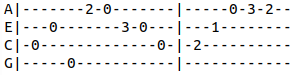
\includegraphics{songs/m/mistersandmantab.png}

\CmajorSeven
\Bseven
\Eseven
\Aseven
\Dseven
\Gseven
\Aminor
\Dminor
\Fminor

\textbf{Riff}\\
Mr. \upchord{Cmaj7}Sandman, \upchord{B7}bring me a dream (bung, bung, bung, bung)\\
\upchord{E7}Make him the cutest that \upchord{A7} I've ever seen (bung, bung, bung, bung)\\
\upchord{D7}Give him two lips like \upchord{G7} roses and clover (bung, bung, bung, bung)\\
\upchord{Cmaj7}Then tell him \upchord{Am}that his lonesome \upchord{D7}nights are \upchord{G7}over\\
\upchord{Cmaj7}Sandman, \upchord{B7}I'm so alone (bung, bung, bung, bung)\\
\upchord{E7}Don't have nobody to \upchord{A7}call my own (bung, bung, bung, bung)\\
\upchord{Dm}Please turn on your magic \upchord{Fm}beam\\
Mr. \upchord{Cmaj7}Sand\upchord{Am}man, \upchord{D7}bring me \upchord{G7}a \upchord{Cmaj7}dream\\
\textbf{Riff}\\
Mr. \upchord{Cmaj7}Sandman, \upchord{B7}bring me a dream\\
\upchord{E7}Make him the cutest that \upchord{A7}I've ever seen\\
\upchord{D7}Give him the word that \upchord{G7}I'm not a rover\\
\upchord{Cmaj7}Then tell him \upchord{Am}that his lonesome \upchord{D7}nights are \upchord{G7}over\\
\upchord{Cmaj7}Sandman, \upchord{B7}I'm so alone (bung, bung, bung, bung)\\
\upchord{E7}Don't have nobody to \upchord{A7}call my own (bung, bung, bung, bung)\\
\upchord{Dm}Please turn on your magic \upchord{Fm}beam\\
Mr. \upchord{Cmaj7}Sand\upchord{Am}man, \upchord{D7}bring me \upchord{G7}a \upchord{Cmaj7}dream\\
\textbf{Riff}\\
Mr. \upchord{Cmaj7}Sandman (yes) \upchord{B7}bring us a dream\\
\upchord{E7}A pair of eyes with a \upchord{A7}"come-hither" gleam\\
\upchord{D7}Give him a lonely heart like \upchord{G7}Pagliacci\\
\upchord{Cmaj7}And lots of wavy \upchord{Am}hair like \upchord{D7}Liberace\upchord{G7}\\
Mr. \upchord{Cmaj7}Sandman, \upchord{B7}someone to hold (someone to hold)\\
\upchord{E7}Would be so peachy \upchord{A7}before we're too old\\
\upchord{Dm}So please turn on your magic \upchord{Fm}beam\\
Mr. \upchord{Cmaj7}Sand\upchord{Am}man, \upchord{D7}bring us\\
Please, \upchord{Cmaj7}please, \upchord{G7}please\\
Mr. \upchord{C}Sand\upchord{Am}man\\
\upchord{D7}Bring us \upchord{G7} a \upchord{Cmaj7}dream\\
\textbf{Riff}\\

\section{The Man Who Sold the World / David Bowie}\label{sec:themanwhosoldtheworld}
\textbf{For bonus marks, for the chords noted "scale", play the major scale instead of the strum. For the C scale, flatten the seventh, i.e. play a Bb instead of a B}

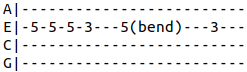
\includegraphics{songs/m/themanwhosoldtheworldtab.png}

\Amajor
\Dminor
\Fmajor
\Aseven
\Cmajor

\textbf{Riff}\\
\upchord{A} \upchord{Dm} \upchord{F} \upchord{Dm}\\
We passed upon the \upchord{A7}stair\\
We spoke of was and when \upchord{Dm}\\
Although I wasn't \upchord{A7}there \\
He said I was his friend \upchord{F}\\
Which came as some sur\upchord{C}prise \\
I spoke into his \upchord{A}eyes, I thought you died a\upchord{Dm}lone\\
A long, long time a\upchord{C scale}go\\
Oh \upchord{C scale}no not \upchord{F scale}me\\
I \upchord{D scale}never lost con\upchord{F scale}trol\\
You're \upchord{C scale}face to \upchord{F scale}face\\
With the \upchord{D riff}man who sold the world\\
\upchord{A} \upchord{Dm} \upchord{F} \upchord{Dm}\\
I laughed and shook his \upchord{A7}hand\\
And made my way back \upchord{Dm}home\\
I searched for form and \upchord{A7}land\\
For years and years I roa\upchord{F}med\\
I gazed a gazely \upchord{C}stare\\
At all the millions \upchord{A}here, we must have died a\upchord{Dm}lone\\
A long, long time a\upchord{C}go\\
Who \upchord{C scale}knows? Not me\upchord{F scale}\\
We \upchord{D scale}never lost con\upchord{F scale}trol\\
You're \upchord{C scale}face to \upchord{F scale}face\\
With the \upchord{D riff}man who sold the world\\
\upchord{A} \upchord{Dm} \upchord{F} \upchord{Dm}\\
Who \upchord{C scale}knows? Not me\upchord{F scale}\\
We \upchord{D scale}never lost con\upchord{F scale}trol\\
You're \upchord{C scale}face to \upchord{F scale}face\\
With the \upchord{D riff}man who sold the world\\
\upchord{A} \upchord{Dm} \upchord{F} \upchord{Dm}\\



%\section{Justified and Ancient / The KLF}\label{sec:justified_and_ancient}
  {\small chords}
  
  \Eminor
  \Dmajor
  \FsharpMinor
  \Gmajor
  \Amajor
  
  \upchord{Bm} All bound for Mu Mu Land, All bound for Mu Mu Land
  \upchord{Bm} \upchord{riff}
  \upchord{Em} All bound for Mu Mu Land
  \upchord{Bm} \upchord{riff}
  \upchord{Em} All bound for Mu Mu Land
  (Bring the beat back!)
  They're \upchord{D} Justified, and they’re \upchord{F#m} Ancient,
  And they \upchord{G} like to roam the \upchord{A} land.
  They're \upchord{D} Justified, and they're \upchord{F#m} Ancient,
  I \upchord{G} hope you under-\upchord{A}-stand.
  They \upchord{G} called me up in \upchord{D} Tennessee
  They said \upchord{G} "Tammy, stand by The \upchord{D} Jams"
  But \upchord{G} if you don't like what they're \upchord{D} going to do,
  You \upchord{A} better not stop them 'cause they're coming through
  \upchord{Bm} \upchord{riff} (Hey hey)
  \upchord{Em} All bound for Mu Mu Land (justified)
  \upchord{Bm} \upchord{riff} (Hey hey)
  \upchord{Em} All bound for Mu Mu Land (justified)
  (Ancients of Mu Mu) (?)
  They're \upchord{D} Justified, and they're \upchord{F#m} Ancient,
  And they \upchord{G} drive an ice cream \upchord{A} van.
  (just roll it from the top)
  They're \upchord{D} Justified and they're \upchord{F#m} Ancient,
  With \upchord{G} still no master \upchord{A} plan.
  The \upchord{G} last train left an \upchord{D} hour ago,
  They were \upchord{G} singing "All a-\upchord{D}-board"
  \upchord{G} All bound for \upchord{D} Mu Mu Land,
  Then \upchord{A} someone starting screaming "Turn up the Strobe"
  (bring the beat back)
  \upchord{Bm} \upchord{riff} (Hey hey)
  \upchord{Em} All bound for Mu Mu Land (justified)
  \upchord{Bm} \upchord{riff} (Hey hey)
  \upchord{Em} All bound for Mu Mu Land
  (Ancients of Mu Mu) (?)
  \upchord{Bm} Justified and Ancient, Ancient and a-justified,
  Rocking to the rhythm in their ice cream van
  with the plan and the key to
  enter into Mu Mu
  Vibes from the tribes of the Jams
  I know where the beat is at,
  'cos I know what time it is
  Bring home a dime,
  Make mine a "99"
  New style, meanwhile, always on a mission while
  Fishing in the rivers of life
  Fishing in the rivers of life (HOI)
  Fishing in the rivers of life (HOI)
  Fishing in the rivers
  Fishing in the rivers
  Fishing in the rivers of life (HOI)
  Voo-va-voolie
  Za-shi-va-zom
  \upchord{Em} Voo-va-voolie (pause)
  (BRING THE BEAT BACK)
  \upchord{Bm} \upchord{riff} (Hey hey)
  \upchord{Em} All bound for Mu Mu Land
  \upchord{Bm} \upchord{riff} (Hey hey)
  \upchord{Em} All bound for Mu Mu Land
  \upchord{single strums - Bm} Mu Mu Land, Mu Mu Land (ANCIENTS OF MU MU, ANCIENTS OF MU MU)
  \upchord{Em} All bound for Mu Mu Land
  \upchord{Bm} Mu Mu Land, Mu Mu Land (ANCIENTS OF MU MU, ANCIENTS OF MU MU)
  \upchord{Em} All bound for Mu Mu Land
  \upchord{a cappella} Mu Mu Land, Mu Mu Land
  All bound for Mu Mu Land


%% END SONGS AM

%\nolinenumbers
% chapter songs_a_m (end)

%\chapter{Songs / N -- Z} % (fold)
%\label{cha:songs_n_z}
%\minitoc
%\Large
%\linenumbers
%\modulolinenumbers[2]

% START SONGS NZ
\section{Nellie the Elephant / The Toy Dolls}\label{sec:nellietheelephant}

\EminorEasy
\Bseven
\Cmajor
\Gmajor
\Bmajor
\FsharpSeven
\EmajorEasy
\Amajor
\BflatMajor
\Fmajor
\Gseven
\Cseven

\textbf{Intro}\\
\upchord{Em} \upchord{B7} \upchord{Em}    \upchord{C} \upchord{B7} \upchord{Em}\\

\textbf{Verse}\\
\upchord{Em}To \upchord{B7}Bom\upchord{Em}bay a \upchord{G}travelling circus \upchord{B}came,\\
They \upchord{F\#7}brought an intelligent \upchord{B}elephant and \upchord{F\#7}Nellie was her \upchord{B}name.\\
\upchord{Em}One \upchord{B7}dark \upchord{Em}night she \upchord{G}slipped her iron \upchord{B}chain\\
And \upchord{F\#7}off she ran to \upchord{B}Hindustan and was \upchord{F\#7}never seen a\upchord{B}gain\\
\textbf{Music Stops}\\
Ooooooooooooooooh\\
\textbf{Chorus: faster}\\
\upchord{E}Nellie the elephant packed her trunk and \upchord{A}said good-bye to the \upchord{E}circus\\
\upchord{A}Off she went with a \upchord{E}trumpety-trump, \upchord{F\#7}TRUMP! \upchord{B7}TRUMP! \upchord{E}TRUMP!\\
Now \upchord{E}Nellie the elephant packed her trunk and \upchord{A}trumbled back to the \upchord{E}jungle\\
\upchord{A}Off she went with a \upchord{E}trumpety-trump, \upchord{F\#7}TRUMP! \upchord{B7}TRUMP! \upchord{E}TRUMP!\\
\textbf{Verse}\\
\upchord{Em}Night \upchord{B7}by \upchord{Em}night, she \upchord{G}danced to the circus \upchord{B}band,\\
When \upchord{F\#7}Nellie was leading the \upchord{B}big parade she \upchord{F\#7}looked so proud and \upchord{B}grand\\
\upchord{Em}No \upchord{B7}more \upchord{Em}tricks for \upchord{G}Nellie to per\upchord{B}form\\
They \upchord{F\#7}taught her how to \upchord{B}take a bow and she \upchord{F\#7}took the crowd by \upchord{B}storm\\
\textbf{Music Stops}\\
Ooooooooooooooooh\\
\textbf{Repeat Chorus}\\
\textbf{After last chord:} \upchord{C}\\
The \upchord{Bb}head of the herd was calling \upchord{F}far, \upchord{Bb}far a\upchord{F}way;\\
they \upchord{G7}met one night in the \upchord{C}silver light on the \upchord{G7}road to Manda\upchord{C}lay\\
\textbf{Music Stops}\\
Ooooooooooooooooh\\
\textbf{Repeat Chorus}\\
\textbf{Outro}\\
\upchord{F} \upchord{Bb} \upchord{F} \upchord{Bb} \upchord{F} \upchord{G7} \upchord{C}\\
\upchord{F} \upchord{Bb} \upchord{F} \upchord{Bb} \upchord{F} \upchord{G7} \upchord{C7} \upchord{F}\\



\section{Party In The USA / Miley Cyrus}\label{sec:partyintheusa}

\Cmajor
\Eminor
\Aminor
\Gmajor
\Dminor
\Fmajor


\textbf{Intro} \\
\upchord{C} \upchord{Em} \upchord{Am} \upchord{G}  x2\\
(\textbf{Verse}). I \upchord{C}hopped off the plane at \upchord{Em}L.A.X.\\
With a \upchord{Am}dream and my cardi\upchord{G}gan\\
\upchord{C}Welcome to the land of \upchord{Em}fame excess,\\
\upchord{Am}Am I gonna fit \upchord{G}in? \upchord{C}Jumped in the cab,\\
Here I \upchord{Em}am for the first time\upchord{Am}\\
Look to my right and I \upchord{G}see the Hollywood sign\\
\upchord{C}This is all so \upchord{Em}crazy \upchord{Am}Everybody seems so \upchord{G}famous\\
(\textbf{Pre-Chorus})\upchord{C}My tummy's turnin' and I'm \upchord{Em}feelin' kinda home sick\upchord{Am}\\
Too much pressure and I'm \upchord{G}nervous,\\
That's when the \upchord{C}taxi man turned on the \upchord{Em}radio\\
And a \upchord{Am}Jay-Z song was \upchord{G}on  \textbf{x3}\\
(\textbf{Chorus}) So I put my \upchord{C}hands up, they're \upchord{Em}playing my song,\\
And the \upchord{Am}butterflies fly a\upchord{G}way\\
I'm \upchord{C}noddin' my head like \upchord{Em}yeah\\
I'm \upchord{Am}movin' my hips like \upchord{G}yeah\\
I got my \upchord{C}hands up,\\
They're \upchord{Em}playing my song,\\
I \upchord{Am}know I'm gonna be O\upchord{G}K\\
\upchord{C}Yeah\upchord{Em}, it's a \upchord{Am}party in the US\upchord{G}A\\
\upchord{C}Yeah\upchord{Em}, it's a \upchord{Am}party in the US\upchord{G}A\\
(\textbf{Verse}) \upchord{C}Get to the club in my \upchord{Em}taxi cab \upchord{Am}Everybody's looking at me \upchord{G}now\\
Like \upchord{C}"Who's that chick, that's \upchord{Em}rockin' kicks?\\
\upchord{Am}She gotta be from out of \upchord{G}town"\\
\upchord{C}So hard with my \upchord{Em}girls not around \upchord{Am}me\\
It's definitely not a \upchord{G}Nashville party\\
\upchord{C}'cause all I see are \upchord{Em}stilettos\upchord{Am}\\
I guess I never got the \upchord{G}memo\\
(\textbf{Pre-Chorus}) \upchord{C}My tummy's turnin' and I'm \upchord{Em}feelin' kinda home sick\upchord{Am}\\
Too much pressure and I'm \upchord{G}nervous,\\
That's when the \upchord{C}D.J. dropped my \upchord{Em}favorite tune\\
and a \upchord{Am}Britney song was \upchord{G}on  \textbf{x3}\\
\textbf{Repeat Chorus}\\
\textbf{Bridge}\\
\upchord{Em}Feel like hoppin' on a \upchord{Am}flight (on a flight)\\
\upchord{Em}Back to my hometown to\upchord{Dm}night (town tonight)\\
\upchord{Em}Something stops me every \upchord{Am}time (every time)\\
\upchord{F}The DJ plays my song and I feel al\upchord{G}right\\
\textbf{Repeat Chorus x 2}\\

\section{Payphone / Maroon 5}\label{sec:payphone}

\CaddNine
\DsusFour
\EminorSeven
\Gmajor

\textbf{Intro} \\                      
I'm at a \upchord{Cadd9}payphone trying to \upchord{G}call home          \\          
All of my \upchord{Em7}change I spent on \upchord{Dsus4}you\\
Where have the \upchord{Cadd9}times gone baby\\
It's \upchord{G}all wrong, where are the \upchord{Em7}plans we made for \upchord{Dsus4}two\\
\textbf{Verse}\\
Yeah, \upchord{Cadd9}I, I know it's hard to remember\\
\upchord{G}The people we used to be. \upchord{Em7}It's even harder to picture\\
\upchord{Dsus4}That you're not here next to me. \upchord{Cadd9}You say it's too late to make it\\
\upchord{G}But is it too late to try? \upchord{Em7}And in our time that you wasted\\
\upchord{Dsus4}All of our bridges burned \upchord{Cadd9}down\\
\textbf{Pre-Chorus}\\
I've wasted my \upchord{G}nights You turned out the \upchord{Em7}lights\\
Now I'm para\upchord{Dsus4}lysed Still stuck in that \upchord{Cadd9}time when we called it \upchord{G}love\\
But even the \upchord{Em7}sun sets in para\upchord{Dsus4}dise\\
\textbf{Chorus}\\
I'm at a \upchord{Cadd9}payphone trying to \upchord{G}call home     \\               
All of my \upchord{Em7}change I spent on \upchord{Dsus4}you\\
Where have the \upchord{Cadd9}times gone baby\\
It's \upchord{G}all wrong, where are the \upchord{Em7}plans we made for \upchord{Dsus4}two\\
If happy ever \upchord{Cadd9}after did exist\upchord{G}\\
I would still be \upchord{Em7}holding you like this\upchord{Dsus4}\\
And all those fairy\upchord{Cadd9}tales are full of stick\upchord{G}\\
One more goddamn \upchord{Em7}love song I'll be sick\upchord{Dsus4}\\
\textbf{Verse}\\
\upchord{Cadd9} You turned your back on tomorrow \upchord{G}Cause you forgot yesterday\\
\upchord{Em7}I gave you my love to borrow \upchord{Dsus4}But you just gave it away\\
\upchord{Cadd9}You can't expect me to be fine \upchord{G} I don't expect you to care\\
\upchord{Em7}I know I've said it before \upchord{Dsus4}But all of our Bridges burned \upchord{Cadd9}down\\
\textbf{Repeat Pre-Chorus}\\
\textbf{Repeat Chorus}\\
Now I'm at a \upchord{Cadd9}payphone\\
\textbf{Verse}\\
man slice that cake \upchord{G}I'll be out spending all this money\\
while you're sitting round \upchord{Em7}Wondering why it wasn't you who came \\
up from nothing \upchord{Dsus4}made it from the bottom mow when you see me I'm stunning\\
\upchord{Cadd9}And all of my cars start with a push of a button\\
\upchord{G}Telling me the chances I blew up or whatever you call it\\
\upchord{Em7}Switched the number to my phone So you never could call it\\
\upchord{Dsus4}Don't need my name on my show You can tell it I'm ballin'\\
\upchord{Cadd9}Swish, what a shame could have got picked\\
\upchord{G}Had a really good game but you missed your last \upchord{Em7}shot\\
So you talk about who you see at the top\\
Or \upchord{Dsus4}what you could have saw But sad to say it's over for\\
\upchord{Cadd9}Phantom pulled up valet open doors\\
\upchord{G}Wiz like go away, got what you was looking for \upchord{Em7}Now it's me who they want\\
So you can go take that little \upchord{Dsus4}piece of cake with you\\
\textbf{Repeat Chorus}\\
Now I'm at a \upchord{Cadd9}payphone\\


\section{Piano Man / Billy Joel}\label{sec:pianoman}

\Cmajor
\Gmajor
\Fmajor
\DmajorSeven
\Aminor
\GmajorSeven
\Amajor
\EmajorEasy
\DmajorEasy
\BmajorSeven
\FsharpMinor


\textbf{Intro} 
\upchord{C} \upchord{G} \upchord{F} \upchord{C} \upchord{F} \upchord{C} \upchord{D7} \upchord{G}  \upchord{C} \upchord{G} \upchord{F} \upchord{C} \upchord{F} \upchord{G} \upchord{C} \upchord{G}\\
It's \upchord{C}nine o'\upchord{G}clock on a \upchord{F}Satur\upchord{C}day\\
The \upchord{F}regular \upchord{C}crowd shuffles \upchord{D7}in\upchord{G}\\
There's an \upchord{C}old man \upchord{G}sitting \upchord{F}next to \upchord{C}me\\
Making \upchord{F}love to his \upchord{G}tonic and \upchord{C}gin\upchord{G}\\
He says, \upchord{C}"Son, can you \upchord{G}play me a \upchord{F}memory\upchord{C}\\
I'm \upchord{F}not really \upchord{C}sure how it \upchord{D7}goes\upchord{G}\\
But it's \upchord{C}sad and it's \upchord{G}sweet and I knew it comp\upchord{F}lete\upchord{C}\\
When \upchord{F}I wore a \upchord{G}younger man's \upchord{C}clothes."\\
\textbf{Interlude}\\
\upchord{Am}la la la, di \upchord{D7}da da\\
\upchord{Am}La la, di di \upchord{D7}da da \upchord{G}dum\upchord{F} \upchord{C} \upchord{G7}\\
\textbf{Chorus}\\
\upchord{C}Sing us a \upchord{G}song, you're the pi\upchord{F}ano man\upchord{C}\\
\upchord{F}Sing us a \upchord{C}song to\upchord{D7}night\upchord{G}\\
Well, we're \upchord{C}all in the \upchord{G}mood for a \upchord{F}melody\upchord{C}\\
And you've \upchord{F}got us all \upchord{G}feeling al\upchord{C}right\upchord{G}\\
Now \upchord{C}John at the \upchord{G}bar is a \upchord{F}friend of \upchord{C}mine\\
He \upchord{F}gets me my \upchord{C}drinks for \upchord{D7}free\upchord{G}\\
And he's \upchord{C}quick with a \upchord{G}joke and he'll \upchord{F}light up your \upchord{C}smoke\\
But there's \upchord{F}some place that \upchord{G}he'd rather \upchord{C}be\upchord{G}\\
He says, \upchord{C}"Bill, I be\upchord{G}lieve this is \upchord{F}killing me."\upchord{C}\\
As the \upchord{F}smile ran a\upchord{C}way from his \upchord{D7}face\upchord{G}\\
"Well I'm \upchord{C}sure that I \upchord{G}could be a \upchord{F}movie star\upchord{C}\\
If \upchord{F}I could get \upchord{G}out of this \upchord{C}place"\\
Now \upchord{C}Paul is a \upchord{G}real estate \upchord{F}novelist\upchord{C}\\
Who \upchord{F}never had \upchord{C}time for a \upchord{D7}wife\upchord{G}\\
And he's \upchord{C}talking with \upchord{G}Davy, who's \upchord{F}still in the \upchord{C}Navy\\
And \upchord{F}probably \upchord{G}will be for \upchord{C}life\upchord{G}\\
And the \upchord{C}waitress is \upchord{G}practicing \upchord{F}politics\upchord{C}\\
As the \upchord{F}businessman \upchord{C}slowly gets \upchord{D7}stoned\upchord{G}\\
Yes, they're \upchord{C}sharing a \upchord{G}drink they \upchord{F}call loneli\upchord{C}ness\\
But it's \upchord{F}better than \upchord{G}drinking a\upchord{C}lone\upchord{G}\\
\textbf{Chorus}\\
It's a \upchord{C}pretty good \upchord{G}crowd for a \upchord{F}Saturday\upchord{C}\\
And the \upchord{F}manager \upchord{C}gives me a \upchord{D7}smile\upchord{G}\\
'Cause he \upchord{C}knows that it's \upchord{G}me they've been \upchord{F}coming to \upchord{C}see\\
To for\upchord{F}get about \upchord{G}life for a \upchord{C}while\upchord{G}\\
And the pi\upchord{C}ano, it \upchord{G}sounds like a \upchord{F}carni\upchord{C}val\\
And the \upchord{F}microphone \upchord{C}smells like a \upchord{D7}beer\upchord{G}\\
And they \upchord{C}sit at the \upchord{G}bar and put \upchord{F}bread in my \upchord{C}jar\\
And say, \upchord{F}"Man, what are \upchord{G}you doing \upchord{C}here?"\upchord{G}\\
\textbf{Interlude}\\
\textbf{Chorus}\\
 

%\section{Radio Ga Ga / Queen}\label{sec:radio_ga_ga}
  {\small / symbols in chorus denote knocking uke. Loads of percussive opportunities here. Probably best during intro and choruses to have three parts: 1 purely percussive and two different strumming. We’ll sort this out at the meeting.}
  
  \Fmajor
  \BflatMajor
  \Gminor
  \Cmajor
  
  \upchord{F} \upchord{Gm} \upchord{Bb} \upchord{Gm} \upchord{Bb} \upchord{F}
  \upchord{F} \upchord{Gm} \upchord{Bb} \upchord{Gm} \upchord{Bb} \upchord{F} \upchord{Bb} \upchord{F} \upchord{Bb}
  \upchord{F}I'd sit alone and watch your light\\
  My \upchord{Gm}only friend through teenage nights\\
  And \upchord{Bb}everything I had to know\\
  I \upchord{Gm}heard it on my \upchord{Bb}ra-\upchord{F}dio\\
  You \upchord{F}gave them all those old time stars\\
  Through \upchord{Gm}wars of worlds - invaded by Mars\\
  You \upchord{Bb}made 'em laugh - you made 'em cry\\
  You \upchord{Gm}made us feel like we c\upchord{Bb}ould \upchord{F}fly (\upchord{Bb}ra - \upchord{F}dio)\\
  So \upchord{F}don't become some background noise\\
  A \upchord{Abdim}backdrop for the girls and boys\\
  Who \upchord{Bb}just don't know or just don't care\\
  And \upchord{G}just complain when you're not there\\
  You \upchord{F}had your time, you had the power\\
  You've \upchord{C}yet to have your finest hour\\
  \upchord{Bb}Ra – \upchord{F}dio, (\upchord{Bb}ra – \upchord{F}dio)\\
  CHORUS:\\
  \upchord{F7}All we hear is \upchord{Bb}radio \upchord{F}ga ga / /\\
  \upchord{Bb}radio \upchord{F}goo goo / / \upchord{Bb}radio \upchord{F}ga ga / /\\
  \upchord{F7}All we hear is \upchord{Bb}radio \upchord{F}ga ga / /\\
  \upchord{Bb}radio \upchord{F}blah blah / /\\
  \upchord{Eb}Radio what's \upchord{Bb}new\upchord{C}?\\
  \upchord{Dm}Radio, \upchord{C}someone still loves\upchord{F} you\\
  We \upchord{F}watch the shows - we watch the stars\\
  On \upchord{Gm}videos for hours and hours\\
  We \upchord{Bb}hardly need to use our ears\\
  How \upchord{Gm}music changes thro\upchord{Bb}ugh the \upchord{F}years\\
  \upchord{F}Let's hope you never leave old friend\\
  Like \upchord{Abdim}all good things on you we depend\\
  So \upchord{Bb}stick around 'cos we might miss you\\
  When \upchord{G7}we grow tired of all this visual\\
  You \upchord{F}had your time - you had the power\\
  You've \upchord{C}yet to have your finest hour\\
  \upchord{Bb}Ra – \upchord{F}dio, (\upchord{Bb}ra – \upchord{F}dio)\\
  (REPEAT CHORUS)\\

\section{Romeo and Juliet / Dire Straits}\label{sec:romeoandjuliet}

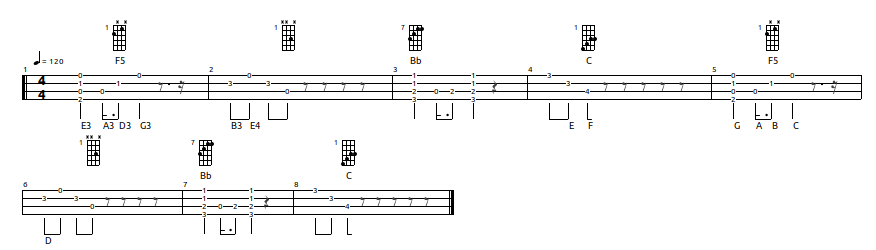
\includegraphics[scale=.6]{songs/r/romeojuliettab.png}
  
  \Fmajor
  \Cmajor
  \BflatMajor
  \Dminor
  
 
\textbf{Intro - use pick above if you like}  \upchord{F} \upchord{C} \upchord{Bb} \upchord{C} x 4\\
 \upchord{F} A lovestruck Romeo \upchord{Dm} sings the streets a sere\upchord{C}nade \upchord{F} \\
 \upchord{F} Laying everybody low \upchord{C} \upchord{Dm} with a love song \upchord{Bb} that he made \upchord{C} Finds a street light \upchord{Bb}\\
 \upchord{C} steps out of the \upchord{F} shade and says something like\\
 \upchord{Bb} You and me babe how a\upchord{C}bout it\\
 \upchord{F} Juliet says hey it's Romeo \upchord{C} \upchord{Dm} you nearly gave me a heart attack \upchord{C} \upchord{F} \\
 \upchord{F} He's underneath the window \upchord{C} she's singing \upchord{Dm} hey la my \upchord{Bb} boyfriend’s back \\
 \upchord{C} You shouldn't come around here \upchord{Bb} \upchord{C} singing up to people like \upchord{F} that \\
 \upchord{Bb} Anyway what you gonna do a\upchord{C}bout it\\
 \textbf{Chorus 1}  \\
 Juli\upchord{F}et \upchord{C} the dice was \upchord{Dm} loaded from the \upchord{Bb} start \\
 \upchord{C} And I \upchord{F} bet \upchord{C} when you ex\upchord{Dm}ploded into my \upchord{Bb} heart\\
 And \upchord{C} I for\upchord{F}get I \upchord{C} for\upchord{Bb}get \upchord{Dm} the movie \upchord{Bb} song\\
 \upchord{Gm} When you gonna realize it was \upchord{Bb} just that the time was \upchord{Dm} wrong \upchord{C}\\
 \upchord{F} Juliet \upchord{C} \upchord{Bb} \upchord{C}  \upchord{F} \upchord{C} \upchord{Bb} \upchord{C} \upchord{F} \\
 Come up on different streets \upchord{Dm} they both were streets of shame \upchord{C} \\
 \upchord{F} \upchord{F} Both dirty both \upchord{C} mean \upchord{Dm} yes and the dream was \upchord{Bb} just the same \upchord{C} \\
 And I dreamed your dream for you \upchord{Bb} \upchord{C} and now your dream is \upchord{F} real \upchord{Bb}\\
 How can you look at me as if I was \upchord{C} just another one of your deals \\
 Well you can \upchord{F} fall for chains of silver \upchord{C} \upchord{Dm} you can fall for chains of gold  \upchord{C} \upchord{F}\\
 \upchord{F}  You can fall for pretty strangers \upchord{C} \upchord{Dm} and the promi\upchord{Bb}ses they hold \upchord{C} \\
 You promised me everything \upchord{Bb} \upchord{C} you promised me \upchord{F} thick and thin yeah \upchord{Bb} \\
 Now you just say oh Romeo yeah you know I \upchord{C} used to have a scene with him \\
 \textbf{Chorus 2}\\
 Juli\upchord{F}et \upchord{C} when we made \upchord{Dm} cake you used to \upchord{Bb} cry\\
 You said I \upchord{F} love you like the \upchord{C} stars above I'll \upchord{Dm} love you till I \upchord{Bb} die \upchord{C}\\
 There's a \upchord{F} place \upchord{C} for \upchord{Bb} us \upchord{Dm} you know the \upchord{Bb} movie song \upchord{Gm}\\
 When you gonna realize it was \upchord{Bb} just that the time was \upchord{Dm} wrong \upchord{C}\\
 Juli\upchord{F}et \upchord{C} \upchord{Bb} \upchord{C}  \upchord{F} \upchord{C} \upchord{Bb} \upchord{C} \upchord{F} \\
 I can't do the talk \upchord{Dm} like they talk on the TV \upchord{C} \upchord{F} \upchord{F} \\
 I can't do a love song \upchord{C} \upchord{Dm} like the way it's \upchord{Bb} meant to be \upchord{C} \\
 I can't do everything \upchord{Bb} \upchord{C} but I'd do anything for \upchord{F} you \upchord{Bb} \\
 I can't do anything except \upchord{C} be in love with you \upchord{F} \\
 And all I do is miss you \upchord{Dm} and the way we used to be  \upchord{C} \upchord{F} \upchord{F}\\
 All I do is keep the beat \upchord{Dm} and bad \upchord{Bb} company \upchord{C} \\
 All I do is kiss you \upchord{Bb} \upchord{C} through the bars of a \upchord{F} rhyme \upchord{Bb} \\
 Juliet I'd do the stars with you \upchord{C} anytime \\
 \textbf{Repeat chorus 2 and half of first verse}  \\

\section{Satellite of Love / Lou Reed}\label{sec:satelliteoflove}

\Gmajor
\Aseven
\Cmajor
\Aminor
\Dseven
\EminorEasy
\Fmajor
\DmajorEasy


\upchord{G} Satellite's \upchord{A7} gone up to the \upchord{Am} skies \upchord{D7}

\upchord{G} Things like that \upchord{A7} drive me out of my \upchord{Am} mind \upchord{D7}

\upchord{Em} I watched it \upchord{D7} for a \upchord{C} little while

\upchord{Am} I like to watch things on \upchord{C} TV

\textbf{Chorus}

\upchord{G} (Bom-bom-bom) Sate\upchord{D}llite of love

\upchord{F} (Bom-bom-bom) Sate\upchord{C} llite of love

\upchord{G} (Bom-bom-bom) Sate\upchord{D}llite of love 

\upchord{Em} Sat\upchord{D}ell\upchord{C}ite \upchord{D} of...

\upchord{G} Satellite's \upchord{A7} gone way up to \upchord{Am} Mars \upchord{D7}

\upchord{G} Soon it'll be \upchord{A7} filled with parking \upchord{Am} cars \upchord{D7}

\upchord{Em} I watched it \upchord{D7} for a \upchord{C} little while \upchord{Am}

I love to watch things on \upchord{C} TV

\textbf{Repeat Chorus}

\upchord{G} I've been \upchord{D7} told that \upchord{Em} you've been \upchord{D7} bold

With \upchord{C} Harry \upchord{D} Mark and \upchord{G} John

\upchord{G} Monday and \upchord{D}Tuesday \upchord{Em} Wednesday to \upchord{D7} Thursday

With \upchord{C} Harry \upchord{D} Mark and \upchord{G} John

\upchord{G} Satellite's \upchord{A7} gone up to the \upchord{Am} skies \upchord{D7}

\upchord{G} Things like that \upchord{A7} drive me out of my \upchord{Am} mind \upchord{D7}

\upchord{Em} I watched it \upchord{D7} for a \upchord{C} little while

\upchord{Am} I love to watch things on \upchord{C} TV

\textbf{Repeat Chorus}

\upchord{G} \upchord{A7} \upchord{C} \upchord{G}

Sate\upchord{A7}llite of \upchord{C} love \upchord{G} (x8)


\section{The Shoop Shoop Song / Rudy Clark}\label{sec:shoop_shoop_song}
% {\small(Girls: don't sing the parts in italics -- Guys: italics are for you)}
\Cmajor
\Fmajor
\Gmajor
\Aminor
\Dminor
\Dseven
\Eseven


\upchord{G}Does he love me \upchord{F}I want to know\\
\upchord{G}How can I tell if he loves me so\\
\emph{(Is it \upchord{Dm}in his \upchord{G}eyes?)} Oh \upchord{Dm}no, you'll be de\upchord{G}ceived\\
\emph{(Is it \upchord{Dm}in his \upchord{G}eyes?)} Oh \upchord{Dm}no he'll make be\upchord{G}lieve\\
If you \upchord{C}wanna \upchord{Am}know if \upchord{F}he loves you \upchord{G}so, it's in his \upchord{C}kiss\\
\emph{\upchord{F}(That's where it \upchord{G}is)} ...Oh yeah\\
\emph{(Is it \upchord{Dm}in his \upchord{G}face?)} Oh \upchord{Dm}no, that's just his \upchord{G}charm\\
\emph{(In his \upchord{Dm}warm em\upchord{G}brace?)} Oh \upchord{Dm}no, that's just his \upchord{G}arms\\
If you \upchord{C}wanna \upchord{Am}know if \upchord{F}he loves you \upchord{G}so, it's in his \upchord{C}kiss \\
\upchord{F}(That's where it \upchord{G}is) ...Oh yeah it's in his \upchord{C}kiss\\
\emph{\upchord{F}(That's where it \upchord{C}is)} Oh, Oh, Oh,\\
\upchord{E7}hug him, squeeze him tight\\
To \upchord{Am}find out what you want to know \upchord{D7}If it's love, if it really is\\
\upchord{G}It's there in his kiss\\
\emph{(How 'bout the \upchord{Dm}way he \upchord{G}acts)}\\
Oh \upchord{Dm}no, that's not the \upchord{G}way\\
\upchord{Dm}You're not \upchord{G}listening to \upchord{Dm}all I \upchord{G}say\\
If you \upchord{C}wanna \upchord{Am}know if \upchord{F}he loves you \upchord{G}so, it's in his \upchord{C}kiss\\
\emph{\upchord{F}(That's where it \upchord{G}is)} oh, oh, it's in his \upchord{C}kiss\\
\emph{\upchord{F}(That's where it \upchord{G}is)}\\
Instrumental:\upchord{Dm}\hrulefill\upchord{G}\hrulefill\upchord{Dm}\hrulefill\upchord{G}\hrulefill\upchord{C}\hrulefill x2\\
\upchord{E7}hug him, squeeze him tight\\
To \upchord{Am}find out what you want to know \upchord{D7}If it's love, if it really is\\
\upchord{G}It's there in his kiss\\
\emph{(How 'bout the \upchord{Dm}way he \upchord{G}acts)} oh \upchord{Dm}no, that's not the \upchord{G}way\\
\upchord{Dm}You're not \upchord{G}listening to \upchord{Dm}all I \upchord{G}say\\
If you \upchord{C}wanna \upchord{Am}know if \upchord{F}he loves you \upchord{G}so, it's in his \upchord{C}kiss\\
\emph{\upchord{F}(That's where it \upchord{G}is)} oh, oh, it's in his \upchord{C}kiss\\
\emph{\upchord{F}(That's where it \upchord{G}is)} oh, oh, it's in his \upchord{C}kiss\\
\emph{\upchord{F}(That's where it \upchord{G}is)} oh yeah, it's in his kiss\\
\upchord{C}\hrulefill\upchord{F}\hrulefill\upchord{C}

\section{Sloop John B / Beach Boys}\label{sec:sloop_john_b}
  {\small chords}
  
  \Cmajor
  \Gseven
  \Dseven
  \Aminor
  
  \upchord{G} We come on the sloop John B\\
  My grandfather and me\\
  Around Nassau town we did \upchord{D7} roam\\
  Drinking all \upchord{G} night \upchord{G7} got into a \upchord{C} fight \upchord{Am}\\
  Well I \upchord{G} feel so broke up \upchord{D7} I want to go \upchord{G} home\\
  Chorus:\\
  \upchord{G} So hoist up the John B’s sail\\
  See how the mainsail sets\\
  Call for the captain ashore let me go \upchord{D7} home\\
  Let me go \upchord{G} home \upchord{G7}\\
  I wanna go \upchord{C} home yeah \upchord{Am} yeah\\
  Well I \upchord{G} feel so broke up \upchord{D7} I wanna go \upchord{G} home\\
  \upchord{G} The first mate he got drunk\\
  And broke in the captain’s trunk\\
  The constable had to come and take him a\upchord{D7}way\\
  Sheriff John \upchord{G} Stone \upchord{G7}\\
  Why don’t you leave me a\upchord{C}lone yeah \upchord{Am} yeah\\
  Well I \upchord{G} feel so broke up \upchord{D7} I wanna go \upchord{G} home\\
  Chorus\\
  \upchord{G} The poor cook he caught the fits\\
  And threw away all my grits\\
  And then he took and he ate up all of my \upchord{D7} corn\\
  Let me go \upchord{G} home \upchord{G7}\\
  Why don’t they let me go \upchord{C} home \upchord{Am}\\
  This \upchord{G} is the worst trip \upchord{D7} I’ve ever been \upchord{G} on\\
  Chorus x 2

\section{Shiny / Jermaine Clement}\label{sec:shiny}

\EminorEasy
\Aminor
\EflatMajor
\Gmajor
\Cmajor
\DmajorEasy
\BflatSeven

\upchord{Em}Well, Tamatoa hasn't always been this glam\\
I was a \upchord{Am}drab little crab once\\
\upchord{Em}Now I know I can be happy as a \upchord{Eb}clam\\
Because I'm beautiful, baby \upchord{Em}\\
Did your granny say listen to your heart\\
Be who you are on the inside\\
I need \upchord{Am}three words to tear her argument a\upchord{Eb}part\\
Your granny lied! I'd rather be \upchord{G}shiny\\
Like a \upchord{C}treasure from a sunken pirate \upchord{G}wreck\\
Scrub the \upchord{C}deck and make it look \upchord{G}shiny\\
I will \upchord{C}sparkle like a wealthy woman's \upchord{Am}neck\\
Just a \upchord{D}sec! Don't you know. //
Fish are \upchord{Em}dumb, dumb, \upchord{C}dumb\\
They chase anything that \upchord{Em}glitters \upchord{C}(beginners!)\\
\upchord{Em}Oh, and here they \upchord{C}come, come, come\\
To the brightest thing that \upchord{Am}glitters\\
Mmm, fish \upchord{D}dinners\\
I just love \upchord{Eb}free food. And you look like seafood \\
Well, well, \upchord{Em}well. Little Maui's having trouble with his look\\
You little \upchord{Am}hemi-demi-semi-god\\
\upchord{Em}Ouch! What a terrible performance. Get the \upchord{Am}hook\\
You don't \upchord{Em}swing it like you used to, man\\
Yet I have to give you credit for my start\\
And your \upchord{Am}tattoos on the out\upchord{Em}side\\
For just like you I made myself a work of \upchord{Eb}art\\
I'll never hide; I can't, I'm too \upchord{G}shiny\\
Watch me \upchord{C}dazzle like a diamond in the \upchord{G}rough\\
Strut my \upchord{C}stuff; my stuff is so \upchord{G}shiny\\
Send your \upchord{C}armies but they'll never be e\upchord{Am}nough. My shell's too \upchord{D}tough\\
Maui man, \upchord{Em}you could try, try, \upchord{C}try\\
But you can't expect a \upchord{Em}demi-god. To beat a \upchord{C}decapod \\
\upchord{Em}You will die, die, \upchord{C}die\\
Now it's time for me to \upchord{Am}take apart your \upchord{D}aching heart\\
\upchord{Eb}Far from the ones who abandoned you\\
Chasing the love of these humans who made you feel wanted\\
You \upchord{Cm}tried to be \upchord{Dm}tough\\
But your \upchord{Eb}armour's just not \upchord{F}hard enough\\
\upchord{Bb}Maui now it's time to kick your \upchord{Bb7}hiney\\
Ever seen someone so \upchord{G}shiny\\
\upchord{C}Soak it in 'cause it's the last you'll ever \upchord{G}see\\
C'est la \upchord{C}vie mon ami. I'm so \upchord{G}shiny\\
Now I'll \upchord{Am}eat you, so prepare your final plea. \upchord{D}Just for me\\
\upchord{Eb}You'll never be quite as shiny\\
You wish you were nice and \upchord{G}shiny


\section{Shotgun / George Ezra}\label{sec:shotgun}

\Fmajor
\BflatMajor
\Dminor
\Cmajor

\textbf{Intro}\\
\upchord{F} \upchord{Bb} \upchord{Dm} \upchord{C}\\
\textbf{Verse}\\
\textbf{single strums}\\
\upchord{F}Home grown alligator \upchord{Bb}see you later\\
Gotta hit the \upchord{Dm}road... gotta hit the \upchord{C}road\\
The \upchord{F}sun and change in the atmosphere \upchord{Bb}architecture unfamiliar\\
\upchord{Dm} I could get used to this \upchord{C}\\
\textbf{Chorus}\\
\textbf{strumming} \upchord{F}Time flies by in the \upchord{Bb}yellow and green\\
Stick a\upchord{Dm}round and you’ll see what I \upchord{C}mean\\
There’s a \upchord{F}mountain top... that \upchord{Bb}I’m dreaming of\\
If you \upchord{Dm}need me, you know where I’ll \upchord{C – single strum}be\\
I’ll be riding \upchord{F}shotgun underneath the \upchord{Bb}hot sun...\\
Feeling like a \upchord{Dm}someone \upchord{C}\\
I’ll be riding \upchord{F}shotgun underneath the \upchord{Bb}hot sun\\
Feeling like a \upchord{Dm}someone \upchord{C}\\
\textbf{Verse}\\
The \upchord{F}south of the equator \upchord{Bb}navigator\\
Gotta hit the \upchord{Dm}road... gotta hit the \upchord{C}road\\
\upchord{F}Deep-sea diving round the clock, bi\upchord{Bb}kini bottoms, lager tops\\
\upchord{Dm} I could get used to this \upchord{C}\\
\textbf{Chorus}\\
\textbf{Verse}\\
We got \upchord{F}two in the front, \upchord{Bb}two in the back\\
\upchord{Dm}Sailing along and we \upchord{C}don’t look ba-a-ack\\
\upchord{F}Ba-a-ack, ba-a-ack, \upchord{Bb}back, back, back\\
\upchord{Dm} \upchord{C}\\
\textbf{Chorus}\\
Feeling like a \upchord{Dm}someone, someone \upchord{C}someone, someone\\
\upchord{F} \upchord{Bb} \upchord{Dm} \upchord{C} \upchord{F}\\

\section{Shout / Isley Brothers}\label{sec:shout}

\Fmajor
\Dminor
\BflatSeven


\textbf{Intro}

We-eee-eeel....      \\                       
You know you make me wanna \upchord{F}(Shout!) Kick my heels up and \upchord{Dm}(Shout!)\\
Throw my hands up and \upchord{F}(Shout!) Throw my head back and \upchord{Dm}(Shout!)\\
Come on now \upchord{F}(Shout!) Don't forget to say you \upchord{Dm}will\\
\upchord{F}Don't forget to say, yeah \upchord{Dm}Yeah, yeah, yeah, yeah\\
\upchord{F}(Say you \upchord{Dm}will) Say it right now bab-ay\\
\upchord{F}(Say you \upchord{Dm}will) Come on, come on\\
\upchord{F}(Say you \upchord{Dm}will) Say it, will-a you-ooooo!\\
\upchord{F}(Say you \upchord{Dm}will) Come on Now\\
\upchord{F}(Say) say that you love me \upchord{Dm}(Say) say that you need me\\
\upchord{F}(Say) say that you want me
\upchord{Dm}(Say) you wanna please me \upchord{F}(Say) come on now \\
\upchord{Dm}(Say) come on now  \upchord{F}(Say) come on now  \upchord{Dm}(Say)...\\
I still re\upchord{F}member (Shooby-doo-wop-do-wop-wop-wop-wop)\\
When you used to be nine years \upchord{Dm}old (Shooby-doo-wop-do-wop-wop-wop-wop) Yeah-yeah!\\
I was a \upchord{F}fool for you, from the bottom of my \upchord{Dm}soul, yeah!\\
(Shooby-doo-wop-do-wop-wop-wop-wop) Now that you've \upchord{F}grown, up\\
(Shooby-doo-wop-do-wop-wop-wop-wop) Up enough to \upchord{Dm}know, yeah yeah\\
(Shooby-doo-wop-do-wop-wop-wop-wop) You wanna \upchord{F}leave me, you wanna, let me \upchord{Dm}go\\
(Shooby-doo-wop-do-wop) I want you to \upchord{F}know\upchord{Bb7}    \upchord{F}\\
I said I \upchord{F}want you to \upchord{Bb7}know \upchord{F}right now, yeah!\upchord{Bb7}        \upchord{F}\\
You been \upchord{Bb7}good to me \upchord{F}baby\upchord{Bb7}\\
\upchord{F}Better than I \upchord{Bb7}been to my\upchord{F}self, hey! hey!\upchord{Bb7}       \upchord{F}\\
And if you \upchord{Bb7}ever leave me\upchord{F} \upchord{Bb7}      \upchord{F}\\
I don't \upchord{Bb7}want nobody \upchord{F}else, hey! hey!\upchord{Bb7}         \upchord{F}\\
I said I \upchord{Bb7}want you to \upchord{F}know-ho-ho-hey!\upchord{Bb7}         \upchord{F}\\
I said I \upchord{Bb7}want you to \upchord{F}know right now, hey! hey!\upchord{Bb7}         \upchord{F}          \upchord{Bb7}\\
You know you \upchord{Bb7}make me wanna \upchord{F}(Shout-wooo) hey-yeah\\
\upchord{Dm}(Shout-wooo) yeah-yeah-yeah \upchord{F}(Shout-wooo) aaaalll-right\\
\upchord{Dm}(Shout-wooo) aaaalll-right\\
\upchord{F}(Shout-wooo) come on now! \upchord{Dm}(Shout) come on now!\\
\upchord{F}(Shout) yeah, yeah, yeah \upchord{Dm}(Shout) yeah, yeah, yeah (good sound)\\
\upchord{F}(Shout) yeah, yeah, yeah (good sound)\\
\upchord{Dm}(Shout) yeah, yeah, yeah (good sound)\\
\upchord{F}(Shout) all-alright (good sound)\\
\upchord{Dm}(Shout) it's all-alright (good sound)\\
\upchord{F}(Shout) all-alright (good sound)\\
\upchord{Dm}(Shout) all-alright (aah) \upchord{F} -STOP- (Shout)\\
Now wai-a-ait A \upchord{F}minute!\\
I feel aaaaaaallllllright! (Yeah-Yeah, Yeah-Yeah, Yeah-Yeah) (OOOOOOOOW)\\	
Now that I got my woman I feel aaaaaaaalllll\upchord{Bb7}right!\\
(Yeah-Yeah, Yeah-Yeah, Yeah-Yeah)\\
Every time I think about you You been so good to me\\
You know you make me wanna\ \upchord{F}(Shout-wooo) lift my heels up and\\
\upchord{Dm}(Shout-wooo) throw my head back and\\
\upchord{F}(Shout-wooo) kick my heels up and\\
\upchord{Dm}(Shout-wooo) come on now \upchord{F}(Shout-wooo) take it easy\\
\upchord{Dm}(Shout-wooo) take it easy \upchord{F}(Shout-wooo) take it easy (higher)\\
\upchord{Dm}(Shout) a little bit softer now (?x)\\
\upchord{F}(Shout) a little bit louder now (?x) (Shout)\\
Hey-HeyA Hey (Hey-HeyA Hey)\\ HeyA HeyA  (HeyA HeyA) (x2) \\
JUMP NOW! Jump up and shout now (wooo)\\
Jump up and shout now (wooo) (x4)\\ 
Everybody shout now Everybody shout now\\
Everybody, shout, shout\\
Shout, shout, shout (x ad lib)\\
Everybody shout now (ooo)\\

\section{Shut Up and Dance With Me / Walk the Moon}\label{sec:shutupanddancewithme}

\Gmajor
\Cmajor
\Fmajor
\Aminor

\textbf{Chorus}

\upchord{G} "Oh don't you \upchord{C} dare look \upchord{F} back.

Just keep your \upchord{Am} eyes on \upchord{G} me."

I said, "You're \upchord{C} holding \upchord{F} back, "

She said, "Shut \upchord{Am} up and \upchord{G} dance with \upchord{C} me!"

This \upchord{F} woman is my \upchord{Am} destiny \upchord{G}

She said, "\upchord{C} Ooh-ooh-\upchord{F} hoo, shut \upchord{Am} up and \upchord{G} dance with \upchord{C} me."

\textbf{Verse 1}

\upchord{F} \upchord{G} \upchord{Am} \upchord{G}  X 2

We were \upchord{C} victims \upchord{F} of the \upchord{Am} night,

The \upchord{G} chemical, \upchord{C} physical, \upchord{F} kryptonite \upchord{Am}

\upchord{G} Helpless to the \upchord{C} bass and the \upchord{F} fading \upchord{Am} light

\upchord{G} Oh, we were \upchord{C} bound to get to\upchord{F}gether, \upchord{Am} bound to get to\upchord{G}gether.


She \upchord{C} took my \upchord{F} arm, I don't know \upchord{Am} how it \upchord{G} happened.

We \upchord{C} took the \upchord{F} floor and she \upchord{G} said,

\textbf{Repeat Chorus}

\textbf{Verse 2}

A backless \upchord{C} dress and some \upchord{F} beat up \upchord{Am} sneaks,

My \upchord{G} discothèque, \upchord{C} Juliet \upchord{F} teenage \upchord{Am} dream.

I \upchord{G} felt it in my \upchord{C} chest as she \upchord{F} looked at \upchord{Am} me. \upchord{G}

I knew we were \upchord{C} bound to be to\upchord{F}gether,

\upchord{Am} Bound to be to\upchord{G}gether

She \upchord{C} took my \upchord{F} arm, I don't know \upchord{Am} how it \upchord{G} happened.

We \upchord{C} took the \upchord{F} floor and she \upchord{C} said,

\textbf{Repeat Chorus}

\textbf{Bridge}

\upchord{F} Oh, come on girl! \upchord{F} \upchord{G} \upchord{Am} \upchord{G}  X 4

\upchord{C} Deep in her \upchord{F} eyes, I think I \upchord{Am} see the \upchord{G} future.

I \upchord{C} realize \upchord{F} this is my last \upchord{G} chance.

She \upchord{C} took my \upchord{F} arm, I don't know \upchord{Am} how it \upchord{G} happened.

We \upchord{C} took the \upchord{F} floor and she \upchord{G} said,

\textbf{Repeat Chorus x 2}


\section{Single Ladies / Beyonce}\label{sec:singleladies}

\Gmajor
\Aminor
\EminorEasy
\Cmajor

\textbf{Just repeat G Am Em C all the way through. Fast}\\
\textbf{Verse}\\
Wah ah \upchord{G}aah a-a \upchord{Am}aah ah, \upchord{Em}waah a-a \upchord{C}aah ah (x a few)\\
All the \upchord{G}single ladies, all the \upchord{Am}single ladies\\
All the \upchord{Em}single ladies, all the \upchord{C}single ladies\\
All the \upchord{G}single ladies, all the \upchord{Am}single ladies\\
All the \upchord{Em}single ladies\\
Now put your \upchord{C}hands up\\
\upchord{G}Up in the club, we \upchord{Am}just broke up\\
I'm \upchord{Em}doing my own little \upchord{C}thing\\
Dec\upchord{G}ided to dip and \upchord{Am}now you wanna trip\\
Cause a\upchord{Em}nother brother noticed \upchord{C}me\\
I'm \upchord{G}up on him, he \upchord{Am}up on me\\
Don't \upchord{Em}pay him any a\upchord{C}ttention\\
Just \upchord{G}cried my tears, for \upchord{Am}three good years\\
Ya \upchord{Em}can't be mad at \upchord{C}me\\
\textbf{Chorus}\\
Cause if you \upchord{G}liked it then you should have put a \upchord{Am}ring on it\\
If you \upchord{Em}liked it then you shoulda put a \upchord{C}ring on it\\
Don't be \upchord{G}mad once you see that \upchord{Am}he want it\\
If you \upchord{Em}liked it then you shoulda put a \upchord{C}ring on it\\
Oh, oh, \upchord{G}oh \upchord{Am} \upchord{Em} \upchord{C}\\
\textbf{Repeat Chorus}\\
\textbf{Verse}\\
I got \upchord{G}gloss on my lips, a \upchord{Am}man on my hips\\
Got me \upchord{Em}tighter in my Dereon \upchord{C}jeans\\
\upchord{G}Acting up, \upchord{Am}drink in my cup\\
I can \upchord{Em}care less what you \upchord{C}think\\
I \upchord{G}need no permission, \upchord{Am}did I mention\\
Don't \upchord{Em}pay him any a\upchord{C}ttention\\
Cause you \upchord{G}had your turn and \upchord{Am}now you gonna learn\\
What it really \upchord{Em}feels like to miss \upchord{C}me\\
\textbf{Chorus x 2}\\
Wah ah \upchord{G}aah a-a \upchord{Am}aah ah, \upchord{Em}waah a-a \upchord{C}aah ah (x a few)\\


\section{Solsbury Hill / Peter Gabriel}\label{sec:solsburyhill}
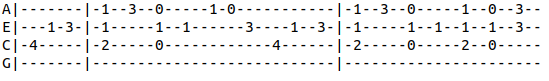
\includegraphics[scale=.6]{songs/s/solsburyhilltab.png}
\Fmajor
\Cmajor
\Dminor
\BflatMajorSeven
\Gminor
\Fmajor
\BflatMajor

\emph{One strum per chord, and the repeated chords are quick ones}\\
\textbf{Do riff a few times to start}\\
\upchord{F} \upchord{C} \upchord{F}\upchord{F} Climbing up on Solsbury Hill\\
\upchord{F} \upchord{C} \upchord{F}\upchord{F} I could see the city light\\
\upchord{Dm} \upchord{C} \upchord{Dm}\upchord{Dm} Wind was blowing, time stood still\\
\upchord{Dm} \upchord{C} \upchord{Dm}\upchord{Dm} Eagle flew out of the night\\
\upchord{F} \upchord{C} \upchord{F}\upchord{F} He was something to observe\\
\upchord{F} \upchord{C} \upchord{F}\upchord{F} Came in close, I heard a voice\\
\upchord{Dm} \upchord{C} \upchord{Dm}\upchord{Dm} Standing stretching every nerve\\
\upchord{Dm} \upchord{C} \upchord{Dm}\upchord{Dm} Had to listen had no \upchord{Bbmaj7}choice\\
I \upchord{C}did not \upchord{Bbmaj7}be\upchord{Bbmaj7}lieve the infor\upchord{Bbmaj7}mation\\
I \upchord{C}just had to \upchord{Bbmaj7} trust imagi\upchord{Bbmaj7}nation\\
My \upchord{C}heart go\upchord{Bbmaj7}ing \upchord{Bbmaj7} boom boom boom\\
\upchord{Bbmaj7}"Son, " he \upchord{C} said \upchord{Bbmaj7} \\
\upchord{Gm}"Grab your \upchord{F}things,\\
I've \upchord{Bb}come to \upchord{C}take you home."\\
\textbf{Riff}\\
\upchord{F} \upchord{C} \upchord{F}\upchord{F} To keep in silence I resigned\\
\upchord{F} \upchord{C} \upchord{F}\upchord{F} My friends would think I was a nut\\
\upchord{Dm} \upchord{C} \upchord{Dm}\upchord{Dm} Turning water into wine\\
\upchord{Dm} \upchord{C} \upchord{Dm}\upchord{Dm} Open doors would soon be shut\\
\upchord{F} \upchord{C} \upchord{F}\upchord{F} So I went from day to day\\
\upchord{F} \upchord{C} \upchord{F}\upchord{F} Tho' my life was in a rut\\
\upchord{Dm} \upchord{C} \upchord{Dm}\upchord{Dm} "Till I thought of what I'd say\\
\upchord{Dm} \upchord{C} \upchord{Dm}\upchord{Dm} Which connection I should cut\\
I was \upchord{C}feeling \upchord{Bbmaj7}part \upchord{Bbmaj7}of the \upchord{Bbmaj7}scenery\\
I \upchord{C}walked right \upchord{Bbmaj7}out of \upchord{Bbmaj7}the machi\upchord{Bbmaj7}nery\\
My \upchord{C}heart go\upchord{Bbmaj7}ing \upchord{Bbmaj7} boom boom boom\\
\upchord{Bbmaj7}"Hey" he \upchord{C} said  \upchord{Bbmaj7} \\
\upchord{Gm}"Grab your \upchord{F}things,\\
I've \upchord{Bb}come to \upchord{C}take you home." Back home\\
\textbf{Riff}\\
\upchord{F} \upchord{C} \upchord{F}\upchord{F} When illusion spin her net\\
\upchord{F} \upchord{C} \upchord{F}\upchord{F} I'm never where I want to be\\
\upchord{Dm} \upchord{C} \upchord{Dm}\upchord{Dm} And liberty she pirouette\\
\upchord{Dm} \upchord{C} \upchord{Dm}\upchord{Dm} When I think that I am free\\
\upchord{F} \upchord{C} \upchord{F}\upchord{F} Watched by empty silhouettes\\
\upchord{F} \upchord{C} \upchord{F}\upchord{F} Who close their eyes but still can see\\
\upchord{Dm} \upchord{C} \upchord{Dm}\upchord{Dm} No one taught them etiquette\\
\upchord{Dm} \upchord{C} \upchord{Dm}\upchord{Dm} I will show another me\\
To\upchord{C}day I don't \upchord{Bbmaj7}need a \upchord{Bbmaj7}replace\upchord{Bbmaj7}ment\\
I'll \upchord{C}tell them \upchord{Bbmaj7}what the \upchord{Bbmaj7}smile on my \upchord{Bbmaj7}face meant\\
My \upchord{C}heart go\upchord{Bbmaj7}ing \upchord{Bbmaj7} boom boom boom\\
\upchord{Bbmaj7}"Hey" I \upchord{C} said  \upchord{Bbmaj7} \\
"You can \upchord{Gm}keep my \upchord{F}things,\\
They've \upchord{Bb}come to \upchord{C}take me home."\\

\section{Song to the Siren / Tim Buckley}\label{sec:songtothesiren}

\Gmajor
\Dmajor
\Cmajor
\Eminor
\Fmajor

\upchord{G}Long afloat on \upchord{D}shipless oceans

\upchord{C}I did all my \upchord{Em}best to smile

\upchord{G}'Til your singing \upchord{D}eyes and fingers

\upchord{C}Drew me loving \upchord{Em}to your isle

\upchord{G}And you sang, \upchord{F}Sail to me, \upchord{Em}Sail to me, Let me en\upchord{G}fold you                        

\upchord{Em}Here I am, \upchord{D}Here I am, \upchord{C}Waiting to \upchord{Em}hold you

\upchord{G}Did I dream \upchord{D}you dreamed about me?

\upchord{C}Were you hare \upchord{Em}when I was fox

\upchord{G}Now my foolish \upchord{D}boat is leaning 

\upchord{C}Broken lovelorn \upchord{Em}on your rocks,

\upchord{G}For you sing, \upchord{F}"Touch me not, touch me \upchord{Em}not, come back to\upchord{G}morrow

\upchord{Em}O my heart\upchord{D}, O my \upchord{C}heart shies from the \upchord{Em}sorrow" 

\upchord{G}I am puzzled \upchord{D}as the oyster

\upchord{C}I am troubled \upchord{Em}as the tide

\upchord{G}Should I stand a\upchord{D}mid your breakers?

\upchord{C}Or should I lie with \upchord{Em}death my bride?

\upchord{G}Hear me sing, \upchord{F}"Swim to me, Swim to \upchord{Em}me, Let me en\upchord{G}fold you

\upchord{Em}Here I am, \upchord{D}Here I am, \upchord{C}

Waiting to \upchord{Em}hold you"


\section{Sound of the Suburbs / The Members}\label{sec:soundofthesuburbs}

\Amajor
\Aminor
\Bmajor
\Cmajor
\Cfive
\DmajorEasy
\EmajorEasy
\Gmajor

\textbf{Intro} \upchord{G} \upchord{G} \upchord{G} \upchord{G} (see intro riff)\\
\upchord{C5} Same old boring Sunday morning, old man's out washing the \upchord{G} car\\
\upchord{C5} Mum's in the kitchen cooking Sunday dinner, her best meal, moaning while it\upchord{G} lasts\\
\upchord{Am} And Johnnys \upchord{C} upstairs in his \upchord{G} bedroom sitting in the dark\\
\upchord{Am} Annoying the \upchord{C} neighbours with his \upchord{G} punk rock electric gui-\upchord{D}-tar /// \upchord{D} /// \upchord{D} /// \upchord{D}\\
This is the \upchord{G} sound, this is the \upchord{B} sound of the \upchord{A} suburbs\\
\upchord{G} This is the \upchord{B} sound of the \upchord{A} suburbs \upchord{C} / \upchord{E} \upchord{D}\\
\upchord{C5} Every lousy Monday morning, Heathrow jets go crashing over our \upchord{G} home\\
\upchord{C5} Ten o'clock, Broadmoor siren, driving me mad, won't leave me a-\upchord{G}-lone\\
\upchord{Am} The woman \upchord{C} next door just \upchord{G} sits there and stares outside\\
\upchord{Am} She hasn't \upchord{C} come out once ever \upchord{G} since her husband \upchord{D}died\\
This is the \upchord{G} sound, this is the \upchord{B} sound of the \upchord{A} suburbs\\
\upchord{G} This is the \upchord{B} sound of the \upchord{A} suburbs \upchord{C} / \upchord{E} \upchord{D}\\
\upchord{E} ///\upchord{E} ///\upchord{G} ///\upchord{G} ///\upchord{E}///\upchord{E} ///\upchord{G} ///\upchord{G} ///\upchord{C} ///\upchord{C} ///\upchord{B} ///\upchord{B} ///\upchord{C} ///\\
\upchord{C}///\upchord{D}-\upchord{D\#}-\upchord{E}-\upchord{F}-\upchord{F\#}-\upchord{G}  \upchord{G\#}-\upchord{A}-\upchord{A\#}-\upchord{B}-\upchord{C}(slide D-bar up the fretboard)\\
\upchord{G} Youth Club groups used to \upchord{B} wanna be free, \upchord{G} now they want \upchord{D} anarchy!\\
They \upchord{G} play too fast, they \upchord{B} play out of tune, \upchord{G} practice in the \upchord{D} singers bedroom\\
\upchord{C} Drums quite good, the bass is too loud, and \upchord{B} I ... can't hear ... the \upchord{A} words\upchord{A}\\
This is the \upchord{G} sound, this is the \upchord{B} sound of the \upchord{A} suburbs\\
\upchord{G} This is the \upchord{B} sound of the \upchord{A} suburbs \upchord{C} / \upchord{E} \upchord{D}\\
\upchord{C5} Saturday morning family shoppers, crowding out...the centre of \upchord{G} town\\
\upchord{C5} Young .. blokes,sitting on the benches, shouting at the young girls, walking a-\upchord{G}-round\\
\upchord{Am} And Johnny \upchord{C} stands there at his \upchord{G} window looking at the night\\
I said\upchord{Am} 'Hey what you \upchord{C} listening to? There's \upchord{G} nothing there!' \upchord{D} That's right.\\
\upchord{G} This is the \upchord{B} sound of the \upchord{A} suburbs\\
\upchord{G} This is the \upchord{B} sound of the \upchord{A} suburbs\\
\upchord{G} \upchord{B} \upchord{A} \upchord{A} \upchord{G} \upchord{B} \upchord{A} \upchord{A}\\
This is the \upchord{G} sound...\upchord{B} ... this is the \upchord{A} sound\\
This is the \upchord{G} sound ... \upchord{B} ... this is the \upchord{A} sound\\
This is the \upchord{G} sound ... \upchord{B} ... this is THE \upchord{A} sound\\
This is the \upchord{G} sound ... \upchord{B} ... this is the \upchord{A} sou-ou-ou-ou-ou-ou-ound\\
\upchord{G} This is the \upchord{B} sound of the \upchord{A} suburbs \upchord{A} (Can you hear?)\\
\upchord{G} This is the \upchord{B} sound of the \upchord{A} suburbs \upchord{A} (Yeah,yeah,yeah,yeah,yeah,yeah,yeah)\\
\upchord{G} This is the \upchord{B} sound of the \upchord{A} suburbs \upchord{A} (The one that I want)\\
\upchord{G} This is the \upchord{B} sound of the \upchord{A} suburbs \upchord{C} / \upchord{E} \upchord{D}\\

\section{Sweet Home Alabama / Lynyrd Skynyrd}\label{sec:sweethomealabama}

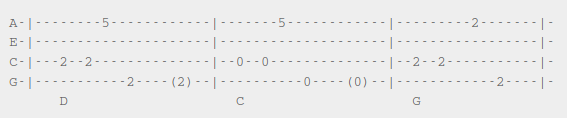
\includegraphics[scale=.6]{songs/s/SweetHomeRiff1.png}\\
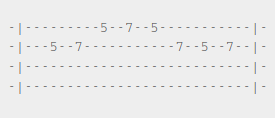
\includegraphics[scale=.6]{songs/s/SweetHomeRiff2.png}

\DmajorEasy
\Cmajor
\Gmajor
\Fmajor

\textbf{Intro}  \\
\upchord{D}\upchord{C}\upchord{G}\upchord{G}x4\\
\textbf{Verse}\\
 \upchord{D}Big \upchord{C}wheels keep on \upchord{G}turning\\
 \upchord{D}Carry me \upchord{C}home to see my \upchord{G} kin\\
 \upchord{D}Singing \upchord{C}songs about the \upchord{G}southland\\
 \upchord{D}I miss ole \upchord{C}'Bamy once \upchord{G}again \upchord{and I think it's a sin}\\
\textbf{Repeat Intro}\\
\textbf{Verse}\\
 \upchord{D}Well, I heard Mister \upchord{C}Young sing a\upchord{G}bout her\\
 \upchord{D}Well, I heard ole \upchord{C}Neil put her \upchord{G}down\\
 \upchord{D}Well, I hope Neil \upchord{C}Young will re\upchord{G}member\\
 \upchord{D}A southern \upchord{C}man don't need him a\upchord{G}round anyhow\\
\textbf{Chorus} \\
 \upchord{D} Sweet \upchord{C}home Ala\upchord{G}bama\upchord{D} \\
 Where the \upchord{C}skies are so \upchord{G}blue\\
 \upchord{D} Sweet \upchord{C}home Ala\upchord{G}bama\\
 \upchord{D} Lord, I'm \upchord{C}coming home to \upchord{G}you\\
\textbf{Verse}\\
 \upchord{D}In Birming\upchord{C}ham they love the \upchord{G}Guvnor\\
 \upchord{F}Boo  \upchord{C}boo  \upchord{D}boo\\
 \upchord{D}Now we all \upchord{C}did what we could \upchord{G}do\\
 \upchord{D}Now Water\upchord{C}gate does not \upchord{G}bother me\\
 \upchord{D}Does your \upchord{C}conscience bother \upchord{G}you?  \upchord{tell the truth}\\
\textbf{Repeat Chorus} \\
 \upchord{D}Now Muscle \upchord{C}Shoals has got the \upchord{G}Swampers\\
 \upchord{D}And they've been \upchord{C}known to pick a song or \upchord{G}two \upchord{yes they do}\\
 \upchord{D}Lord they \upchord{C}get me off \upchord{G}so much\\
 \upchord{D} They pick me \upchord{C}up when I'm feeling \upchord{G}blue \upchord{now how about you?}\\
\textbf{Repeat Chorus} \\
 \upchord{D} (single strum)\\

\section{Teenage Dirtbag / Wheatus}\label{sec:teenagedirtbag}
\Cmajor
\BflatMajor
\Dminor
\DminorSeven
\DminorSix
\Fmajor
\Gseven



\textbf{intro}    \\
\upchord{F} \upchord{C} \upchord{F} \upchord{Bb}x2\\
Her \upchord{F}name is No\upchord{C}elle... \\
\upchord{F}I have a \upchord{Bb}dream about her\upchord{F}She rings my \upchord{C}bell... \\
I got \upchord{F}gym class in \upchord{Bb}half an hour\upchord{F}Oh how she \upchord{C}rocks...\\
in \upchord{F}keds and tube \upchord{Bb}socks\\
But \upchord{Dm}she doesn’t \upchord{Bb}know who I \upchord{Csus4}am \\
\upchord{C}And \upchord{Dm}she doesn’t \upchord{Bb}give a \upchord{Csus4}damn a\upchord{C}bout me\\
Cos \upchord{F}I’m just a \upchord{Bb}teenage \upchord{C}dirtbag \upchord{Dm}baby \\
\upchord{Am}Yeah \upchord{F}I’m just a \upchord{Bb}teenage \upchord{C}dirtbag \upchord{Dm}baby \\
\upchord{Am}\upchord{F}Listen to \upchord{Bb}Iron \upchord{C}Maiden \upchord{Dm}baby, \upchord{Am}with \upchord{F}me \\
\upchord{Bb}Ooo-ooo \upchord{C}oooh\upchord{Dm-Dm} \\
\upchord{Am-Am} \upchord{Bb-Bb}\upchord{C-C}\\
Her \upchord{F}boyfriend’s a \upchord{C}dick... \\
\upchord{F}he brings a \upchord{Bb}gun to school\\
And \upchord{F}he’d simply \upchord{C}kick... \\
my \upchord{F}ass if he \upchord{Bb}knew the truth\\
He \upchord{F}lives on my \upchord{C}block... \\
and \upchord{F}drives an I\upchord{Bb}ROC\\
But \upchord{Dm}he doesn’t \upchord{Bb}know who I \upchord{Csus4}am \\
\upchord{C}And \upchord{Dm}he doesn’t \upchord{Bb}give a \upchord{Csus4}damn a\upchord{C}bout me\\
Cos \upchord{F}I’m just a \upchord{Bb}teenage \upchord{C}dirtbag \upchord{Dm}baby \\
\upchord{Am}Yeah \upchord{F}I’m just a \upchord{Bb}teenage \upchord{C}dirtbag \upchord{Dm}baby \\
\upchord{Am}\upchord{F}Listen to \upchord{Bb}Iron \upchord{C}Maiden \upchord{Dm}baby, \upchord{Am}with \upchord{F}me\\
\upchord{Bb}Ooo-ooo \upchord{C}oooh\\
\upchord{Dm-Dm} \upchord{Am-Am} \upchord{Bb-Bb}\upchord{C-C}\\
\upchord{F}\upchord{Bb}Oh yeaaa-\upchord{F}-ah\upchord{Bb}dirtbaaaa-\upchord{F}-aaa-\upchord{Bb}-ag\\
No \upchord{Dm}she does\upchord{Am}n’t know \upchord{Bb}what she’s \upchord{C}missing\\
%F}\upchord{Bb}Oh yeaaa-\upchord{F}-ah\upchord{Bb}dirtbaaaa-\upchord{F}-aaa-\upchord{Bb}-ag\\
No \upchord{Dm}she does\upchord{Am}n’t know \upchord{Bb}what she’s \upchord{C}missing\\
\upchord{F} \upchord{C} \upchord{F} \upchord{Bb}x2\\
Man \upchord{F}I feel like \upchord{C}mould... \\
it’s \upchord{F}prom night and \upchord{Bb}I am lonely\\
\upchord{F}Lo and be\upchord{C}hold... \\
\upchord{F}she’s walking \upchord{Bb}over to me\\
\upchord{F}This must be \upchord{C}fake... \\
my \upchord{F}lip starts to \upchord{Bb}shake\\
\upchord{Dm}How does she \upchord{Bb}know who I \upchord{Csus4}am? \\
\upchord{C}And \upchord{Dm}why does she \upchord{Bb}give a \upchord{Csus4}damn a\upchord{C}bout me?\\
I’ve got two \upchord{F}tickets to \upchord{Bb}Iron \upchord{C}Maiden \upchord{Dm}baby \\
\upchord{Am}\upchord{F}Come with me \upchord{Bb}Friday \upchord{C}don’t say \upchord{Dm}maybe \\
\upchord{Am}\upchord{F}I’m just a \upchord{Bb}teenage \upchord{C}dirtbag \upchord{Dm}baby, \upchord{Am}like \upchord{F}you\\
\upchord{Bb}\upchord{C}\upchord{Dm-Dm} \upchord{Am-Am} \upchord{Bb-Bb}\upchord{C-C}\\
\upchord{F}\upchord{Bb}Oh yeaaa-\upchord{F}-ah\upchord{Bb}dirtbaaaa-\upchord{F}-aaa-\upchord{Bb}-ag\\
No \upchord{Dm}she does\upchord{Am}n’t know \upchord{Bb}what she’s \upchord{C}missing\\
\upchord{F}\upchord{Bb}Oh yeaaa-\upchord{F}-ah\upchord{Bb}dirtbaaaa-\upchord{F}-aaa-\upchord{Bb}-ag\\
No \upchord{Dm}she does\upchord{Am}n’t know \upchord{Bb}what she’s \upchord{C}missing\\
\upchord{F} \upchord{C}... \upchord{F} \upchord{Bb}... \upchord{F} \upchord{C}... \\
\upchord{Dm-Dm} \upchord{Am-Am} \upchord{Bb-Bb}\upchord{C-C}\\
\upchord{F –single strum}\\


\section{That's Not My Name / Ting Tings}\label{sec:thatsnotmyname}
\DmajorEasy
\Fmajor
\Gmajor
\Amajor

\emph{On this one, you should play the D chord by fingering an F chord, then adding your 3rd and 4th fingers on the C and E strings 2nd fret to make the annoying D shape. Then you can just lift them off when you need to do the quick Fs in the verse. You mainly play D and G in this - you have to try to make it percussive.}

\textbf{Verse}\\
\upchord{D}Four little words just to get me along \upchord{F-D}\\
\upchord{D}It's a difficulty and I'm biting on my tongue \upchord{F-D}and I\\
\upchord{D}I keep stalling, keeping me together \upchord{F-D}\\
\upchord{D}People around gotta find something to say now \upchord{F-D}\\
\upchord{D}Holding back, everyday the same \upchord{F-D}\\
\upchord{D}Don't wanna be a loner. Listen to me, oh no \upchord{F-G}\\
\upchord{G}I never say anything at all \upchord{F-G}\\
\upchord{G}But with nothing to consider\\
They forget my \upchord{A}name (ame, ame, ame) \upchord{F-D}\\
\textbf{Chorus}\\
\upchord{D}They call me "hell" \upchord{F-D}. \upchord{D}They call me "Stacey" \upchord{F-D}\\
\upchord{D}They call me "her" \upchord{F-D}. \upchord{D}They call me "Jane" \upchord{F-G}\\
\upchord{G}That's not my name. \upchord{G}That's not my name \upchord{F-G}\\
\upchord{G}That's not my name. \upchord{G}That's not my name \upchord{F-D}\\
\upchord{D}They call me "quiet gal"\upchord{F-D}. \upchord{D}But I'm a riot \upchord{F-D}\\
\upchord{D}Mary, Jo, Lisa \upchord{F-D}. \upchord{D}Always the same \upchord{F-G}\\
\upchord{G}That's not my name \upchord{F-G}. \upchord{G}That's not my name \upchord{F-G}\\
\upchord{G}That's not my name \upchord{F-G}. \upchord{G}That's not my name \upchord{F-D}\\
\textbf{Verse 2}\\
\upchord{D}I miss the catch if they throw me the ball \upchord{F-D}\\
\upchord{D}I'm the last chick standing up against the wall \upchord{F-D}\\
\upchord{D}Keep up, falling, these heels they keep me boring \upchord{F-D}\\
\upchord{D}Getting glammed up and sitting on the fence now \upchord{F-D}\\
\upchord{D}So alone all the time at night \upchord{F-D}\\
\upchord{D}Lock myself away. Listen to me, oh no \upchord{F-G}\\
\upchord{G}Although I'm dressed up, out and all with \upchord{F-G}\\
\upchord{G}Everything considered\\
They forget my \upchord{A}name (ame, ame, ame) \upchord{F-D}\\
\textbf{Repeat Chorus}\\
\upchord{D}Are, you, cal - ling, me, \upchord{G}dar - ling ? \upchord{G-A}\\
\upchord{D}Are, you, cal - ling, me, \upchord{G}bi - rd ? \upchord{G-A}\\
\upchord{D}Are, you, cal - ling, me, \upchord{G}dar - ling ? \upchord{G-A}\\
\upchord{D}Are, you, cal - ling, me, \upchord{G}bi - rd ? \upchord{G-A}\\
\textbf{Chorus ad lib}



\section{Tiny Dancer / Elton John}\label{sec:tinydancer}

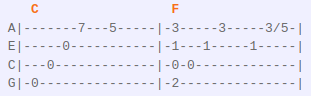
\includegraphics[scale=.6]{songs/t/TinyDancerRiff.png}


\Cmajor
\Fmajor
\Gmajor
\EminorSeven
\AminorSeven
\Dminor
\Eseven
\Aminor
\Gseven

\textbf{Intro}\upchord{C}\upchord{F}\upchord{C}\upchord{F}\\
\textbf{Verse}\\
\upchord{C}Blue jean \upchord{F}baby,\upchord{C}L.A.\upchord{F}lady\\
\upchord{C}Se\upchord{Am}stress for the \upchord{F}band  \upchord{F}   \upchord{G}\\
\upchord{C}Pretty \upchord{F}eyed, \upchord{C}pirate \upchord{F}smile\\
\upchord{C}You’ll \upchord{C}marry a music\upchord{F} man \upchord{F}  \upchord{G}\\
\\
\textbf{Bridge}\\
\upchord{F}Baller\upchord{Em7}ina,  \upchord{Am7}you must have \upchord{D}seen her\\
\upchord{Dm}    \upchord{E7}Dancing in the \upchord{Am}sand   \upchord{G7}\
\upchord{C}And now she’s \upchord{F}in me, \upchord{C}always \upchord{F}with me\\
\upchord{C}Tiny \upchord{C}dancer in my \upchord{G}hand   \upchord{F}    \upchord{Em7}      \upchord{Dm}\\
\\
\textbf{Repeat Intro}\\
\textbf{Verse}\\
\upchord{C}Jesus \upchord{F}freaks \upchord{C}out on the \upchord{F}street\\
\upchord{C}Handing t\upchord{C}ickets out for \upchord{F}God   \upchord{F} \upchord{G}\\
\upchord{C}Turning \upchord{F}back \upchord{C}she just \upchord{F}laughs\\
\upchord{C}The boule\upchord{C}vard is not that \upchord{F}bad   \upchord{F}     \upchord{G}\\
\\
\textbf{Bridge}\\
\upchord{F}Piano \upchord{Em7}man \upchord{Am7}he makes his \upchord{D}stand\\
\upchord{Dm}In the \upchord{E7}auditori\upchord{Am}um     \upchord{G7}\\
\upchord{C}Looking \upchord{F}on   \upchord{C}she sings the \upchord{F}songs\\
\upchord{C}The words she \upchord{C}knows the tune she \upchord{G}hums   \upchord{F}   \upchord{Em7}   \upchord{Dm}\\
\textbf{Repeat Intro}\\
\\
\textbf{Pre-Chorus}\\
\upchord{G\♯}But oh how it \upchord{A\♯}feels so real\\
\upchord{Gm}Lying here with \upchord{Cm}no one near\\
\upchord{G\♯}Only you\upchord{G\♯} and you can \upchord{A\♯}hear me\\
\upchord{A\♯}When I say \upchord{G}softly \upchord{G7}slowly\\
\\
\textbf{Chorus}\\
\upchord{F}Hold me \upchord{C}closer tiny \upchord{Dm}dancer  \upchord{Dm}    \upchord{Em7}\\
\upchord{F}Count the \upchord{C}headlights on the \upchord{G}highway   \upchord{G}    \upchord{Em7}\\
\upchord{F}Lay me \upchord{C}down in sheets of \upchord{Dm}linen    \upchord{Dm}   \upchord{Em7}\\
\upchord{F}You had a \upchord{C}busy day Gtoday      \upchord{G}\\


\section{Total Eclipse of the Heart / Bonnie Tyler}\label{sec:totaleclipseoftheheart}
\Bminor
\Amajor
\DmajorEasy
\Cmajor
\Fmajor
\BflatMajor
\Bmajor
\EmajorEasy
\FsharpMinor
\Fminor

\upchord{Bm}TURN AROUND Every now and then I get a \upchord{A}little bit lonely and you're never coming
round.

\upchord{Bm}TURN AROUND Every now and then I get a \upchord{A}little bit tired of listening to the sound of
my tears.

\upchord{D}TURN AROUND Every now and then I get a \upchord{C}little bit nervous that the best of all the
years have gone by.

\upchord{D}TURN AROUND Every now and then I get a \upchord{C}little bit terrified and then I see the look in
your eyes.

\upchord{F}TURN AROUND, \upchord{Bb}BRIGHT EYES Every now and then I fall apart.

\upchord{F}TURN AROUND, \upchord{Bb}BRIGHT EYES Every now and then I fall apart.

\upchord{Bm}TURN AROUND Every now and then I get a \upchord{A}little bit restless and I dream of
something wild.

\upchord{Bm}TURN AROUND Every now and then I get a \upchord{A}little bit helpless and I'm lying like
a child in your arms.

\upchord{D}TURN AROUND Every now and then I get a \upchord{C}little bit angry and I know I've got to
get out and cry.

\upchord{D}TURN AROUND Every now and then I get a \upchord{C}little bit terrified but then I see the
look in your eyes.

\upchord{F}TURN AROUND, \upchord{Bb}BRIGHT EYES Every now and then I fall apart.

\upchord{F}TURN AROUND, \upchord{Bb}BRIGHT EYES Every now and then I fall \upchord{A}apart.

\upchord{A}And I \upchord{F#m}need you now \upchord{D}tonight and I \upchord{E}need you more than \upchord{A}ever

And if you \upchord{F#m}only hold me \upchord{D}tight we'll be \upchord{E}holding on for\upchord{A}ever.

And we'll \upchord{F#m}only be making it \upchord{D}right 'cause we'll \upchord{E}never be wrong.

\upchord{D}Together we can take it to the \upchord{E}end of the line.

Your \upchord{F#m}love is like a shadow on me \upchord{B}all of the time.

I \upchord{A}don't know what to do and I'm \upchord{E}always in the dark.

We're \upchord{F#m}living in a powder keg and \upchord{B}giving off sparks.

I really need you \upchord{D}tonight, \upchord{B}forever's gonna start \upchord{D}tonight,

For\upchord{E}ever's gonna start tonight

\upchord{A}Once upon a time I was \upchord{F#m}falling in love but \upchord{C#m}now I'm only falling \upchord{D}apart.

There's \upchord{Bm}nothing I can do, a\upchord{E}total eclipse of the heart.

\upchord{A} \upchord{F#m}\upchord{D} \upchord{E}

\upchord{A}Once upon a time there was \upchord{F#m}light in my life but \upchord{C#m}ow there's only love

the \upchord{D}dark.\upchord{A}

\upchord{Bm}Nothing I can say, a \upchord{E}total eclipse of the \upchord{A}heart.

\upchord{Bm} \upchord{A}

\upchord{Bm} \upchord{A}

\upchord{D} \upchord{C}

\upchord{D} \upchord{C}

\upchord{F}TURN AROUND, \upchord{Bb}BRIGHT EYES Every now and then I fall apart.

\upchord{F}TURN AROUND, \upchord{Bb}BRIGHT EYES Every now and then I fall \upchord{A}apart.

\upchord{A}And I \upchord{F#m}need you now tonight \upchord{D}and I \upchord{E}need you more than \upchord{A}ever

And if you \upchord{F#m}only hold me \upchord{D}tight we'll be \upchord{E}holding on for\upchord{A}ever.

And we'll \upchord{F#m}only be making it \upchord{D}right 'cause we'll \upchord{E}never be wrong.

\upchord{D}Together we can take it to the \upchord{E}end of the line.

Your \upchord{F#m}love is like a shadow on me \upchord{B}all of the time.

I \upchord{A}don't know what to do and I'm \upchord{E}always in the dark.

We're \upchord{F#m}living in a powder keg and \upchord{B}giving off sparks.

I really need you \upchord{D}tonight, \upchord{B}forever's gonna \upchord{C#m}start \upchord{D}tonight,

For\upchord{E}ever's gonna start tonight.

\upchord{A}Once upon a time I was \upchord{F#m}falling in love but \upchord{C#m}now I'm only falling \upchord{D}apart.

There's \upchord{Bm}nothing I can do, a\upchord{E}total eclipse of the heart.

\upchord{A} \upchord{F#m} \upchord{D} \upchord{E}

\upchord{A}Once upon a time there was \upchord{F#m}light in my life but \upchord{C#m}now there's only love

the \upchord{D}dark.\upchord{A}

\upchord{Bm}Nothing I can say, a \upchord{E}total eclipse of the \upchord{A}heart. \upchord{A} \upchord{F#m} \upchord{D} \upchord{E}

Song fades out on:

\upchord{A}Turn around, \upchord{F#m}bright eyes \upchord{D} \upchord{E}

\section{Twist and Shout / The Beatles}\label{sec:twistandshout}
\Dmajor
\Gmajor
\Aseven

\upchord{D} \upchord{G} \upchord{A7} - Same chords throughout the song\\
Well shake it up baby \upchord{D} now, (\upchord{G} shake it up \upchord{A7} baby)\\
Twist and \upchord{D} shout. (\upchord{G} Twist and \upchord{A7} shout)\\
Come on, come on, come on, come on, \upchord{D} baby now (\upchord{G} come on \upchord{A7} baby)\\
Come on and work it on \upchord{D} out. (\upchord{G} Work it on \upchord{A7} out, ooh!)\\

Well work it on out honey (work it on out)\\
You know you look so good. (Look so good)\\
You know you got me goin’ now, (Got me goin’)\\
Just like I knew you would. (Like I knew you would, ooh!)\\

Well shake it up baby now, (shake it up baby)\\
Twist and shout. (Twist and shout)\\
Come on, come on, come on, come on, baby now, (come on baby)\\
Come on and work it on out. (Work it on out, ooh!)\\

You know you twist it little girl,(twist little girl)\\
You know you twist so fine. (Twist so fine)\\
Come on and twist a little closer now, (twist a little closer)\\
And let me know that you’re mine. (Let me know you’re mine, ooh!)\\

\upchord{D} \upchord{G} \upchord{A7}  x4\\
\upchord{A} Ahh ahh \upchord{A7} ahh ahh ahh yeah!!\\

\upchord{D} \upchord{G} \upchord{A7}\\

Shake it up baby \upchord{D} now, (\upchord{G} shake it up \upchord{A7} baby)\\

Twist and shout. (Twist and shout)\\
Come on, come on, come on, come on, baby now, (come on baby)\\
Come on and work it on out. (Work it on out, ooh!)\\
You know you twist it little girl, (twist little girl)\\
You know you twist so fine. (Twist so fine)\\
Come on and twist a little closer now, (twist little closer)\\
And let me know that you’re mine. (Let me know you’re mine ooh!)\\

Well shake it shake it shake it baby now. (shake it up baby)\\
Well shake it shake it shake it baby now. (shake it up baby)\\
Well shake it shake it shake it baby now. (shake it up baby)\\

\upchord{A} \upchord{A7} Ahh ahh ahh ahh \upchord{A} \upchord{Bb} \upchord{B} \upchord{C} \upchord{C#} \upchord{D} \upchord{D7}\\

(just a barre chord slide up)\\


%\section{The Times They Are a-Changin' / Bob Dylan}\label{sec:times_they_are_a_changin}
\Cmajor
\Dmajor
\Gmajor
\Aminor
\Eminor

Come \upchord{G}gather round \upchord{Em}people \upchord{C}wherever you \upchord{G}roam

And \upchord{G}admit that the \upchord{Em}waters \upchord{C}around you have \upchord{D}grown

And \upchord{G}accept it that \upchord{Em}soon you'll be \upchord{C}drenched to the \upchord{G}bone

If your \upchord{G}time to \upchord{Am}you is worth \upchord{D}savin'

So you \upchord{D}better start \upchord{C}swimming or you'll \upchord{G}sink like a \upchord{D}stone

For the \upchord{G}times, they \upchord{C}are a-\upchord{D}chang-\upchord{G}in'\\


Come \upchord{G}writers and \upchord{Em}critics who \upchord{C}prophesise with your \upchord{G}pen 

And \upchord{G}keep your eyes \upchord{Em}wide the chance \upchord{C}won't come \upchord{D}again

And \upchord{G}don't speak too \upchord{Em}soon for the wheel's \upchord{C}still in \upchord{G}spin

And there's \upchord{G}no tellin' \upchord{Am}who that it's \upchord{D}namin'

For the \upchord{D}loser \upchord{C}now will be \upchord{G}later to \upchord{D}win

For the \upchord{G}times they \upchord{C}are a-\upchord{D}chang\upchord{G}in'\\


Come \upchord{G}mothers and \upchord{Em}fathers \upchord{C}throughout the \upchord{G}land

And \upchord{G}don't criti\upchord{Em}cize what you \upchord{C}don't under \upchord{D}stand

Your \upchord{G}sons and your \upchord{Em}daughters are \upchord{C}beyond your \upchord{G}command

Your \upchord{G}old road is \upchord{Am}rapidly \upchord{D}agin'

Please \upchord{D}get out of the \upchord{C}new one if you \upchord{G}can't lend a \upchord{D}hand

For the \upchord{G}times they \upchord{C}are a- \upchord{D}chan\upchord{G}gin'\\


Come \upchord{G}senators, \upchord{Em}congressmen \upchord{C}please heed the \upchord{G}call

Don't \upchord{G}stand in the \upchord{Em}doorway, don't \upchord{C}block up the \upchord{D}hall

For \upchord{G}he that gets \upchord{Em}hurt will be \upchord{C}he who has \upchord{G}stalled

There's a \upchord{G}battle out \upchord{Am}side and it's \upchord{D}ragin'

It'll \upchord{D}soon shake your \upchord{C}windows and \upchord{G}rattle your \upchord{D}walls

For the \upchord{G}times they \upchord{C}are a- \upchord{D}chang\upchord{G}in'\\


The \upchord{G}line it is \upchord{Em}drawn the \upchord{C}curse it is \upchord{G}cast

The \upchord{G}slow one \upchord{Em}now will \upchord{C}later be \upchord{D}fast

As the \upchord{G}present \upchord{Em}now will \upchord{C}later be \upchord{G}past

The \upchord{G}order is \upchord{Am}rapidly \upchord{D}fadin'

And the \upchord{D}first one \upchord{C}now will \upchord{G}later be \upchord{D}last

For the \upchord{G}times they \upchord{C}are a- \upchord{D}chang\upchord{G}in'
%\section{William Harker / Skinny Lister / George Thomas}\label{sec:william_harker}
  {\small chords}
  
  \Cmajor
  \Aminor
  \Dmajor
  
  Me \upchord{G} name is William Harker I'm a rake and a roarin' blade
  \upchord{C} Revelry is \upchord{G} my delight and \upchord{Am} roguery's me \upchord{D} trade
  If you \upchord{G} chuck a penny in the ole grey goose you're sure to hit a nail
  \upchord{C} There's no one that \upchord{G} I have done, no \upchord{Am} friendship \upchord{D} I've be\upchord{G}trayed
  CHORUS
  And it's \upchord{G} hold me hand me hearties, step with the heel and toe
  \upchord{C} Rolling down, \upchord{G} strolling down to the \upchord{Am} public house we'll \upchord{D} go
  We've a \upchord{G} flute and a fiddle and a derry down diddle, and a rattle on the ole
  banjo
  \upchord{C} Rolling down, \upchord{G} strolling down to the \upchord{Am} public \upchord{D} house we'll \upchord{G} go
  VERSE 2
  I've \upchord{G} kissed some girls in Belgium, I've cuddled some girls in Spain
  But the \upchord{C} girls I kiss on a \upchord{G} Saturday night are the \upchord{Am} girls I'd kiss \upchord{D}
  again
  When we \upchord{G} cut a caper on the bar room floor for neither lust nor gain
  If \upchord{C} we're not lovers when we're \upchord{G} homeward bound, it’s \upchord{Am} good friends
  \upchord{D} we'll \upchord{G} remain
  >>>Repeat CHORUS<<<
  VERSE 3
  I've \upchord{G} got a dog named Barker, he likes a drop of beer
  He \upchord{C} gets right drunk, rolls \upchord{G} on the floor and he \upchord{Am} grins from ear to \upchord{D}
  ear
  And by \upchord{G} day you'll see us walking over woodland, hill and vale
  \upchord{C} Every night we'll \upchord{G} both get tight on \upchord{Am} Mrs \upchord{D} Sturgen's \upchord{G} ale
  INSTRUMENTAL - \upchord{G} / \upchord{C} / \upchord{G} / \upchord{Am} / \upchord{D} / \upchord{G} / \upchord{C} / \upchord{G} / \upchord{Am} / \upchord{D} / \upchord{G}
  VERSE 4
  Now \upchord{G} some like a cool clear larger, others like a bottle of pale
  The \upchord{C} boys all titter at a \upchord{G} pint of bitter and some \upchord{Am} drink Anstell's \upchord{D}
  ale (God help them!)
  I'm \upchord{G} pegging out for a jet black stout, it's beauty to aspire
  With me \upchord{C} hand the bar I'll \upchord{G} swear Ooo-arr! I'll \upchord{Am} drink it \upchord{D} till I \upchord{G} die
  >>>Repeat CHORUS<<< (slow down at last line to end)

\section{Waka Waka (This Time For Africa) / Shakira}\label{sec:wakawaka}

  \Cmajor
  \Gmajor
  \Aminor
  \Fmajor
  
  
\textbf{Intro} \\
\upchord{C} x loads

You're a good soldier, \upchord{G}choosing your battles\\
\upchord{Am}Pick yourself up and dust yourself \upchord{F}off, get back in the saddle\\
\upchord{C}You're on the frontline, \upchord{G}everyone's watching\\
\upchord{Am}You know it's serious, we're getting \upchord{F}closer, this isn't over\\
\upchord{C}The pressure's on, \upchord{G}you feel it\\
\upchord{Am}But you got it all, \upchord{F}believe it\\
\upchord{C}When you fall get up, oh, oh\\
\upchord{G}And if you fall get up, eh, eh\\
\upchord{Am}Tsamina mina zangalewa \upchord{F}'cause this is Africa\\
\upchord{C}Tsamina mina, eh, eh\\
\upchord{G}Waka waka, eh, eh\\
\upchord{Am}Tsamina mina zangalewa\\
\upchord{F}This time for Africa\\
\upchord{C}\upchord{G}\upchord{Am}\upchord{F} x2 (two strikes each chord)\\
\upchord{C}Listen to your God, \upchord{F}this is our motto\\
\upchord{Am}Your time to shine, don't wait in \upchord{F}line, y vamos por todo\\
\upchord{C}People are raising \upchord{G}their expectations\\
\upchord{Am}Go on and feed them, this is your \upchord{F}moment, no hesitation\\
\upchord{C}Today's your day, \upchord{G}I feel it\\
\upchord{Am}You paved the way, \upchord{F}believe it\\
\upchord{C}If you get down get up, oh, oh\\
\upchord{G}When you get down get up, eh, eh\\
\upchord{Am}Tsamina mina zangalewa\\
\upchord{F}This time for Africa\\
\upchord{C}Tsamina mina, eh, eh\\
\upchord{G}Waka waka, eh, eh\\
\upchord{Am}Tsamina mina zangalewa, \upchord{F}anawa-a-a\\
\upchord{C}Tsamina mina, eh, eh\\
\upchord{G}Waka waka, eh, eh\\
\upchord{Am}Tsamina mina zangalewa\\
\upchord{F}This time for Africa


\section{We Are Never Ever Getting Back Together / Taylor Swift}\label{sec:weareneverevergettingbacktogether}

  \Cmajor
  \Gmajor
  \DmajorEasy
  \EminorSeven
  
  
\upchord{C} I remember when we broke \upchord{G} up the first time\\
\upchord{D} Saying, "This is it, I've had \upchord{Em7} enough," 'cause like\\
\upchord{C} We hadn't seen each other in a \upchord{G} month\\
When you \upchord{D} said you needed \upchord{Em7} space. What?\\
 \\
\upchord{C} Then you come around again and \upchord{G} say\\
"Baby, I \upchord{D} miss you and I swear I'm gonna \upchord{Em7} change\\
Trust me, \upchord{C} remember how that lasted for a \upchord{G} day"\\
I say, "I \upchord{D} hate you, we break up," you \upchord{Em7} call me, "I love you".\\
 \\
\upchord{C} Oooh \upchord{G} oh …we \upchord{D} called it off \upchord{Em7} again last night\\
But \upchord{C} oooh \upchord{G} oh …, this \upchord{D} time I'm \upchord{Em7} telling you, I'm telling you.\\
 \\
\textbf{Chorus} \upchord{C} We are \upchord{G} never ever \upchord{D} ever getting\upchord{Em7} back to-\upchord{D} gether\\
\upchord{C} We are \upchord{G} never ever \upchord{D} ever getting \upchord{Em7} back to-\upchord{D} gether\\
\upchord{C} You go talk to \upchord{G} your friends, talk to my \upchord{D} friends, talk to \upchord{Em7} me \upchord{D}\\
But \upchord{C} we are \upchord{G} never ever \upchord{D} ever ever \upchord{Em7} getting back to-\upchord{C} gether, \upchord{G} like \upchord{D} ever...\upchord{Em7}\\
\\
I'm \upchord{C} really gonna miss you picking \upchord{G} fights\\
And me, \upchord{D} falling for it screaming that I'm \upchord{Em7} right\\
And you, \upchord{C} would hide away and find your piece of \upchord{G} mind\\
With some \upchord{D} indie record that's much \upchord{Em7} cooler than mine.\\
 \\
\upchord{C} Oooh \upchord{G} oh …we \upchord{D} called it off \upchord{Em7} again last night\\
But \upchord{C} oooh \upchord{G} oh …, this \upchord{D} time I'm \upchord{Em7} telling you, I'm telling you.\\
 \\
\textbf{Repeat Chorus}\\
\textbf{Bridge} \upchord{C} I used to \upchord{G} think that \upchord{D} we were for-\upchord{Em7} ever ever ever\\
And \upchord{C} I used to \upchord{G} say \upchord{D} never say \upchord{Em7} never\\
\upchord{C} Huh, so he \upchord{G} calls me up and he's like, "I still \upchord{D} love you"\\
And I'm \upchord{Em7} like, "I just, I mean \upchord{C} this is exhausting, you \upchord{G} know\\
We are never getting \upchord{D} back together, like ever".\\
\textbf{Repeat Chorus x 2}  \\

\section{What's Up? / 4 Non Blondes}\label{sec:whatsup}

  \Gmajor
  \Aminor
  \Cmajor
  
  
\textbf{Intro} \\
\upchord{G}\upchord{Am} \upchord{C}\upchord{G}\upchord{G}\\
25 years of my life and still\\
\upchord{Am}Trying to get up that great big hill of\upchord{C}Hope\\
For a desti\upchord{G}nation\\
I \upchord{G}realised quickly when I knew I should\\
That the \upchord{Am}world was made for this brotherhood of \upchord{C}man\\
For whatever that \upchord{G}means\\
\textbf{Chorus}\\
And so I \upchord{G}cry sometimes when I'm lying in bed\\
Just to \upchord{Am}get it all out, what's in my head\\
And I, \upchord{C} I'm feeling\\
A little pe\upchord{G}culiar\\
And so I \upchord{G}wake in the morning and I step outside\\
And I \upchord{Am}take deep breath and I get real high\\
And I \upchord{C}scream to the top of my lungs what's goin' \upchord{G}on?\\
And I say \upchord{G}hey-yeah-yeah-yeah \upchord{Am}Hey yeah yeah\\
I say \upchord{C}hey\\
What's goin'\upchord{G}on?\\
And I say \upchord{G}hey-yeah-yea-eah, \upchord{Am}Hey yeah yeah\\
I say \upchord{C}hey\\
What's goin' \upchord{G}on?\\
\upchord{G}Oooh, oo!  oo oo-\upchord{Am}Oo-hoo hoo hoo hoo hoo hoo hoo hoo\\
\upchord{C}Oooh! ...ooo-hoo-hoo-ah-\upchord{G}ha\\
And I \upchord{G}try\\
Oh my God do I \upchord{Am}try\\
I try all the \upchord{C}time\\
In this insti\upchord{G}tution\\
And I \upchord{G}pray, Oh my God do I \upchord{Am}pray\\
I pray every single \upchord{C}day\\
For revo\upchord{G}lution\\
\textbf{Repeat Chorus}\\
\textbf{Single Strums}\\
\upchord{G}25 years of my life and still\\
\upchord{Am}Trying to get up that great big hill of\\
\upchord{C}Hope.... for a desti\upchord{G}nation\\

\section{When I'm Gone / Anna Kendrick}\label{sec:whatsup}

\Cmajor
\Fmajor
\Aminor
\Gmajor

  

\upchord{C}I got my ticket for the \upchord{C}long way 'round\\
\upchord{F}Two bottle o' whiskey for the \upchord{C}way\\
And I \upchord{Am}sure would like \upchord{G}some \upchord{F}sweet company\\
And I'm \upchord{Dm}leavin' to\upchord{G}morrow, what you \upchord{C}say?\\
When I'm \upchord{Am}gone, When I'm \upchord{F}gone\\
\upchord{Am}You're gonna miss me when I'm \upchord{G}gone\\
You're gonna \upchord{Am}miss me by my \upchord{G}hair\\
You're gonna \upchord{F}miss me everywhere, oh\\
\upchord{Dm}You're gonna \upchord{G}miss me when I'm \upchord{C}gone\\
When I'm \upchord{Am}gone, When I'm \upchord{F}gone\\
\upchord{Am}You're gonna miss me when I'm \upchord{G}gone\\
You're gonna \upchord{Am}miss me by my \upchord{G}walk\\
You're gonna \upchord{F}miss me by my talk, oh\\
\upchord{Dm}You're gonna \upchord{G}miss me when I'm \upchord{C}gone\\
\upchord{C} x4\\
\upchord{C}I got my ticket for the \upchord{C}long way 'round\\
\upchord{F}The one with the prettiest of \upchord{C}views\\
It's got \upchord{Am}mountains, it's got \upchord{G}rivers\\
It's got \upchord{F}sights to give you shivers\\
But it \upchord{Dm}sure would be \upchord{G}prettier with \upchord{C}you\\
When I'm \upchord{Am}gone, When I'm \upchord{F}gone\\
\upchord{Am}You're gonna miss me when I'm \upchord{G}gone\\
You're gonna \upchord{Am}miss me by my \upchord{G}walk\\
You're gonna \upchord{F}miss me by my talk, oh\\
\upchord{Dm}You're gonna \upchord{G}miss me when I'm \upchord{C}gone\\
When I'm \upchord{Am}gone, When I'm \upchord{F}gone\\
\upchord{Am}You're gonna miss me when I'm \upchord{G}gone\\
You're gonna \upchord{Am}miss me by my \upchord{G}hair\\
You're gonna \upchord{F}miss me everywhere, oh\\
\upchord{Dm}You're gonna \upchord{G}miss me when I'm \upchord{C}gone\\
When I'm \upchord{Am}gone, When I'm \upchord{F}gone\\
\upchord{Am}You're gonna miss me when I'm \upchord{G}gone\\
You're gonna \upchord{Am}miss me by my \upchord{G}walk\\
You're gonna \upchord{F}miss me by my talk, oh, \upchord{Dm}\\
You're gonna \upchord{G}miss me when I'm \upchord{C}gone


\section{When Will My Life Begin? / From \emph{Enchanted}}\label{sec:whenwillmylifebegin}

\Amajor
\DmajorEasy
\BflatMajor
\Fmajor
\Bminor
\Eseven
\Eminor



\textbf{Intro}\\
\upchord{A}  \upchord{D}  \upchord{A}  \upchord{D}  \upchord{A}  \upchord{D}\\
\upchord{A}Seven AM, the usual morning \upchord{D}lineup\\
\upchord{A}Start on the chores and sweep 'til the floor's all \upchord{D}clean\\
\upchord{Bb}Polish and wax, do laundry, and mop and s\upchord{F}hine up\\
Sweep a\upchord{A}gain, and by \upchord{D}then it's like \upchord{E7}seven fif\upchord{A}teen\\
And so I'll \upchord{D}read a \upchord{G}book\\
Or maybe \upchord{Em}two or \upchord{D}three\\
I'll add a \upchord{Bm}few new \upchord{Em}paintings to my \upchord{G}galle\upchord{D}ry\\
I'll play \upchord{Bm}guitar and \upchord{Em}knit\\
And cook and \upchord{G}ba\upchord{D}sica\upchord{Bm}lly\\
Just wonder \upchord{E7}when will my \upchord{A}life be\upchord{D}gin?\\
\upchord{A}  \upchord{D}  \upchord{A}  \upchord{D}\\
\upchord{A}Then after lunch it's puzzles and darts and \upchord{D}baking\\
\upchord{A}Paper mache, a bit of ballet and \upchord{D}chess\\
\upchord{Bb}Pottery and ventriloquy, candle ma\upchord{F}king\\
Then I'll \upchord{A}stretch, maybe \upchord{D}sketch, take a \upchord{E7}climb\\
Sew a \upchord{A}dress!\\
And I'll \upchord{D}re-read the \upchord{G}books\\
If I have \upchord{Em}time to \upchord{D}spare\\
I'll paint the \upchord{Bm}walls some \upchord{Em}more\\
I'm sure there's \upchord{G}room some\upchord{D}where\\
And then I'll \upchord{Bm}brush and \upchord{Em}brush\\
And brush and \upchord{G}brush \upchord{D}my h\upchord{Bm}air\\
Stuck in the \upchord{Em}same place I've \upchord{G}al\upchord{D}ways \upchord{Bm}been\\
\upchord{A}nd I'll keep \upchord{Em}wanderin' and \upchord{D}wanderin'\\
\upchord{A}nd \upchord{G}wanderin' and \upchord{D}wonde\upchord{Bm}rin'\\
\upchord{Em}When will my l\upchord{A}ife be\upchord{D}gin?\\
\textbf{Single strum entire last verse}\\
Tomorrow \upchord{G}night\\
The \upchord{D}lights will ap\upchord{G}pear\\
\upchord{D}Just like they \upchord{G}do on my \upchord{D}birthday \upchord{G}each year\upchord{A}\\
\upchord{Bm}What is it \upchord{E7}like\\
\upchord{A} \upchord{D}\\
Out there where they glow?\\
\upchord{G}Now that I'm \upchord{D}older\\
Mother \upchord{G}might just\\
Let me \upchord{A}go...\\

\section{Where Is My Mind / Pixies}\label{sec:whereismymind}

\Fmajor
\Dminor
\Amajor
\BflatMajor 


{\small{The pick is GCE strings, A string, E string, A string for each of the chords save the last B flat where you lift your finger off the E string and on again. If someone fancies doing the whistle as well, that would work.}}

\textbf{Intro}

\upchord{F} \upchord{Dm} \upchord{A} \upchord{Bb}

\textbf{Verse 1}

With your \upchord{F}feet in the air and your \upchord{Dm}head on the ground \upchord{A} \upchord{Bb}

\upchord{F}Try this \upchord{Dm}trick and \upchord{A}spin it, \upchord{Bb}yeah

\upchord{F}Your head will coll\upchord{Dm}apse

But there's \upchord{A}nothing in it 

And you'll \upchord{Bb}ask yourself

\textbf{Chorus}

\upchord{F}Where is my \upchord{Dm}mind?

\upchord{A}Where is my \upchord{Bb}mind?  

\upchord{F}Where is my \upchord{Dm}mind? \upchord{A} \upchord{Bb}

\textbf{Repeat Intro}

\textbf{Bridge}

\upchord{F}Way \upchord{A}out in the \upchord{Bb}water, see it \upchord{Bbm}swimming.\upchord{Dm}\upchord{C}

\textbf{Verse 2}

\upchord{F}I was \upchord{Dm}swimmin' \upchord{A}in the \upchord{Bb}Carribean\upchord{Bb}

\upchord{F}Animals were \upchord{Dm}hiding behind the \upchord{A}rock\upchord{Bb}

\upchord{F}Except the little \upchord{Dm}fish

But they \upchord{A}told me, he swears

They were \upchord{Bb}trying to talk to me

\textbf{Repeat Chorus}

\textbf{Repeat Bridge}

\textbf{Repeat Verse 1}

\textbf{Repeat Chorus}

\textbf{Repeat Intro}

\textbf{Repeat Bridge}

\section{You're Welcome / Lin-Manuel Miranda, Dwayne Johnson}\label{sec:yourewelcome}
  
\Aminor
\Fmajor
\Cmajor
\Gmajor
  
\upchord{Am}OK, OK, I \upchord{F}see what's happening \upchord{C}here\\
You're \upchord{G}face to face with greatness, and it's \upchord{Am}strange\\
You don't even \upchord{F}know how you feel\\
It's a\upchord{C}dorable\\
Well, it's \upchord{G}nice to see that humans never \upchord{Am}change\\
Open your \upchord{F}eyes, let's be\upchord{C}gin\\
Yes, it's really \upchord{G}me, it's Maui\\
Breathe it \upchord{Am}in\\
I know it's a \upchord{F}lot\\
The hair, the \upchord{C}bod\\
When you're \upchord{G}staring at a demi-god\\
\upchord{Am}What can I \upchord{F}say except, "You're \upchord{C}welcome"\\
For the \upchord{G}tides, the sun, the \upchord{Am}sky\\
Hey, it's o\upchord{F}kay, it's okay\\
You're \upchord{C}welcome\\
I'm \upchord{G}just an ordinary demi-\upchord{Am}guy\\
Hey, what has two \upchord{F}thumbs and pulled up the \upchord{C}sky\\
When you were waddling \upchord{G}yay high? This guy!\\
\upchord{Am}When the nights got \upchord{F}cold\\
Who stole you \upchord{C}fire from down below?\\
You're \upchord{G}lookin' at him, yo\\
\upchord{Am}Oh, also I \upchord{F}lassoed the \upchord{C}sun (you're welcome!)\\
To \upchord{G}stretch your days and bring you \upchord{Am}fun\\
Also I \upchord{F}harnessed the \upchord{C}breeze (you're welcome!)\\
To \upchord{G}fill your sails and shake your trees\\
\upchord{Am}So what can I \upchord{F}say except you're \upchord{C}welcome\\
For the \upchord{G}islands I pulled from the \upchord{Am}sea\\
There's no need to \upchord{F}pray, it's okay, you're \upchord{C}welcome\\
Ha, I \upchord{G}guess it's just my way of being \upchord{Am}me\\
You're \upchord{F}welcome, you're \upchord{C}welcome\\
\upchord{G}Well, come to think of it \upchord{Am}Kid, honestly I could go on and on\\
\upchord{F}I could explain every natural phenomenon \upchord{C}The tide, the grass, the ground\\
\upchord{G}Oh, that was Maui just messing around \upchord{Am}I killed an eel, I buried its guts\\
\upchord{F}Sprouted a tree, now you got coconuts \upchord{C}What's the lesson? What is the take-away?\\
\upchord{G}Don't mess with Maui when he's on a break-away \upchord{Am}And the tapestry here on my skin\\
\upchord{F}Is a map of the victories I win \upchord{C}Look where I've been I make everything happen\\
\upchord{Am}Look at that mean mini-Maui just \upchord{F}tippity-tappin'\\
\upchord{C}(Ha ha ha ha ha \upchord{G} ha, hey)\\
\upchord{Am}Well, any\upchord{F}way let me say, "You're \upchord{C}welcome" (you're welcome)\\
For the \upchord{G}wonderful world you \upchord{Am}know\\
Hey, it's o\upchord{F}kay, it's okay, you're \upchord{C}welcome (you're welcome)\\
Well, \upchord{G}come to think of it, I gotta \upchord{Am}go (hey)\\
Hey, it's your \upchord{F}day to say, "You're \upchord{C}welcome" (you're welcome)\\
'Cause \upchord{G}I'm gonna need that \upchord{Am}boat\\
I'm sailing a\upchord{F}way, away, you're \upchord{C}welcome (you're welcome)\\
'Cause \upchord{G}Maui can do anything but \upchord{Am}float\\
You're \upchord{F}welcome, you're \upchord{C}welcome.\\
You're welcome, and thank you \upchord{C}\\




%\section{Wuthering Heights / Kate Bush}\label{sec:wuthering_heights}
  {\small chords}
  
  \Fmajor
  \Emajor
  \CsharpMajor
  \AflatMajor
  \Dminor
  \Gmajor
  \Cmajor
  
  \upchord{A} Out on the wily, \upchord{F} windy moors, we’d \upchord{E} roll and
  fall in \upchord{C\#} green.//
  \upchord{A} You had a temper \upchord{F} like my jealou-\upchord{E}-sy, too hot,
  too \upchord{C\#} greedy.//
  \upchord{A} How could you leave me, \upchord{F} when I needed to \upchord{E}
  possess you? \upchord{C\#} I hated you. \upchord{Ab} I loved you, too.//
  \upchord{A few players strumming}//
  \upchord{F} Bad dreams in the \upchord{E} night. \upchord{F} You told me I was
  \upchord{E} going to lose the fight. \upchord{F} Leave behind my \upchord{E}
  Wuthering, Wuthering, Wuthering Heights.//
  \upchord{Everyone strumming}//
  Heath-\upchord{F}-cliff, \upchord{Dm} it’s \upchord{G} me, I’m Cathy, I’ve come
  \upchord{C} home. \upchord{F} I ́m so cold, let me \upchord{G} in-a-your \upchord{C} win\upchord{F}-dow.//
  Heath-\upchord{F}-cliff, \upchord{Dm} it’s \upchord{G} me, I’m Cathy, I’ve come
  \upchord{C} home. \upchord{F} I ́m so cold, let me \upchord{G} in-a-your \upchord{C} win\upchord{F}-dow.//
  \upchord{A} Ooh, it gets dark! \upchord{F} It gets lonely, \upchord{E} on the
  other \upchord{C\#} side from you.//
  \upchord{A} I pine a lot. \upchord{F} I find the lot \upchord{E} faster with \upchord{C\#}
  out you.//
  \upchord{A} I’m coming back, love, \upchord{F} cruel Heathcliff, \upchord{E} my
  one dream, \upchord{C\#} my only \upchord{Ab} master.//
  \upchord{F} Too long I \upchord{E} roamed in the night.//
  \upchord{F} I’m coming back to his \upchord{E} side, to put it right.//
  \upchord{F} I’m coming home to \upchord{E} Wuthering, Wuthering,
  Wuthering Heights.//
  Heath-\upchord{F}-cliff, \upchord{Dm} it’s \upchord{G} me, I’m Cathy, I’ve come
  \upchord{C} home. \upchord{F} I ́m so cold, let me \upchord{G} in-a-your \upchord{C} win\upchord{F} dow.//
  Heath-\upchord{F}-cliff, \upchord{Dm} it’s \upchord{G} me, I’m Cathy, I’ve come
  \upchord{C} home. \upchord{F} I ́m so cold, let me \upchord{G} in-a-your \upchord{C} win\upchord{F}-dow//
  \upchord{Am} Ooh! Let me \upchord{G} have it.//
  Let me \upchord{F} grab your \upchord{G} soul away.//
  \upchord{Am} Ooh! Let me \upchord{G} have it.//
  Let me \upchord{F} grab your \upchord{G} soul away.//
  \upchord{Am} You know it’s \upchord{G} me, Cath-\upchord{F}-y!//
  Heath-\upchord{F}-cliff, \upchord{Dm} it’s \upchord{G} me, I’m Cathy, I’ve come
  \upchord{C} home. \upchord{F} I ́m so cold, let me \upchord{G} in-a-your \upchord{C} win-
  \upchord{F}-dow.//
  Heath-\upchord{F}-cliff, \upchord{Dm} it’s \upchord{G} me, I’m Cathy, I’ve come
  \upchord{C} home. \upchord{F} I ́m so cold, let me \upchord{G} in-a-your \upchord{C} win-
  \upchord{F}-dow.//
  Heath-\upchord{F}-cliff, \upchord{Dm} it’s \upchord{G} me, I’m Cathy, I’ve come
  \upchord{C} home. \upchord{F} I ́m so cold...//
  \upchord{Single strum:} \upchord{F}//
  \upchord{Dm} \upchord{G} \upchord{C}, cha cha cha//

%\section{YMCA / Village People}\label{sec:ymca}
  {\small chords}
  
  \Aminor
  \Fmajor
  \Gseven
  
  \upchord{C} Young man there's no need to feel down\\
  I said \upchord{Am} young man pick yourself off the ground\\
  I said \upchord{F} young man cause you're in a new town\\
  There's no \upchord{G7} need to be unhappy\\
  \upchord{C} Young man there's a place you can go\\
  I said \upchord{Am} young man when you're short on your dough\\
  You can \upchord{F} stay there and I'm sure you will find\\
  Many \upchord{G7} ways to have a good time (1,2,3,4,5..)\\
  Chorus: It's fun to stay at the \upchord{C} YMCA it's fun to stay at the \upchord{Am} YMCA\\
  They have \upchord{F} everything for young men to enjoy\\
  You can \upchord{G7} hang out with all the boys\\
  It's fun to stay at the \upchord{C} YMCA it's fun to stay at the \upchord{Am} YMCA\\
  You can \upchord{F} get yourself cleaned you can have a good meal\\
  You can \upchord{G7} do whatever you feel\\
  \upchord{C} Young man are you listening to me\\
  I said \upchord{Am} young man what do you want to be\\
  I said \upchord{F} young man you can make real your dreams\\
  But you \upchord{G7} got to know this one thing\\
  \upchord{C} No man does it all by himself\\
  I said \upchord{Am} young man put your pride on the shelf\\
  And just \upchord{F} go there to the YMCA\\
  I'm \upchord{G7} sure they can help you today (1,2,3,4,5..)\\
  \upchord{C} Young man I was once in your shoes\\
  I said \upchord{Am} I was down and out with the blues\\
  I felt \upchord{F} no man cared if I were alive\\
  I felt \upchord{G7} the whole world was so tight\\
  That's when \upchord{C} someone came up to me\\
  And said \upchord{Am} young man take a walk up the street\\
  There's a \upchord{F} place there called the YMCA\\
  They can \upchord{G7} start you back on your way (1,2,3,4,5..)\\
  Chorus x 2

% END SONGS NZ

\nolinenumbers
% chapter songs_n_z (end)

% \chapter{Appendix A: New Songs} % (fold)
% \label{prt:appendix_a}
% \minitoc
% \Large
% \linenumbers
% \modulolinenumbers[2]
% START SONGS APPENDIX_A

% END SONGS APPENDIX_A
% \nolinenumbers
 %chapter appendix_a (end)

\end{document}
